\documentclass[11pt,reqno]{amsart}

\usepackage[citation-order]{amsrefs}%

\usepackage[utf8]{inputenc}
\usepackage[pdfborder={0 0 0.5 [3 2]}, plainpages=false]{hyperref}%
\usepackage[left=1in,right=1in,top=1in,bottom=1in]{geometry}%

\usepackage{amsmath, amssymb, amsfonts, amsthm, mathtools}
\usepackage{enumerate}
\usepackage{bbm}
\usepackage{booktabs}
\usepackage[table,xcdraw]{xcolor}
\usepackage{float}
\usepackage{cool}
\usepackage{url}
\usepackage{graphicx,epsfig}
\usepackage{makecell}
\usepackage{array}

\usepackage{blkarray}
\usepackage{multirow}

\usepackage[capitalize,nameinlink]{cleveref}
% Per SIAM Style Manual, "section" should be lowercase
\crefname{section}{section}{sections}
\crefname{subsection}{subsection}{subsections}
\Crefname{section}{Section}{Sections}
\Crefname{subsection}{Subsection}{Subsections}

% Per SIAM Style Manual, "Figure" should be spelled out in references
\Crefname{figure}{Figure}{Figures}

% Per SIAM Style Manual, don't say equation in front on an equation.
\crefformat{equation}{\textup{#2(#1)#3}}
\crefrangeformat{equation}{\textup{#3(#1)#4--#5(#2)#6}}
\crefmultiformat{equation}{\textup{#2(#1)#3}}{ and \textup{#2(#1)#3}}
{, \textup{#2(#1)#3}}{, and \textup{#2(#1)#3}}
\crefrangemultiformat{equation}{\textup{#3(#1)#4--#5(#2)#6}}%
{ and \textup{#3(#1)#4--#5(#2)#6}}{, \textup{#3(#1)#4--#5(#2)#6}}{, and \textup{#3(#1)#4--#5(#2)#6}}

% But spell it out at the beginning of a sentence.
\Crefformat{equation}{#2Equation~\textup{(#1)}#3}
\Crefrangeformat{equation}{Equations~\textup{#3(#1)#4--#5(#2)#6}}
\Crefmultiformat{equation}{Equations~\textup{#2(#1)#3}}{ and \textup{#2(#1)#3}}
{, \textup{#2(#1)#3}}{, and \textup{#2(#1)#3}}
\Crefrangemultiformat{equation}{Equations~\textup{#3(#1)#4--#5(#2)#6}}%
{ and \textup{#3(#1)#4--#5(#2)#6}}{, \textup{#3(#1)#4--#5(#2)#6}}{, and \textup{#3(#1)#4--#5(#2)#6}}

% Make number non-italic in any environment.
\crefdefaultlabelformat{#2\textup{#1}#3}

% For vectors (and some matrices?)
\newcommand{\vvec}{\mathbf{v}}
\newcommand{\Avec}{\mathbf{A}}
\newcommand{\Gvec}{\mathbf{G}}
\newcommand{\Hvec}{\mathbf{H}}

\newcommand{\Ivec}{\mathbf{I}}
\newcommand{\Jvec}{\mathbf{J}}
\newcommand{\Kvec}{\mathbf{K}}
\newcommand{\Mvec}{\mathbf{M}}
\newcommand{\Uvec}{\mathbf{U}}
\newcommand{\Vvec}{\mathbf{V}}
\newcommand{\evec}{\mathbf{e}}
\newcommand{\uvec}{\mathbf{u}}
\newcommand{\xvec}{\mathbf{x}}
\newcommand{\mvec}{\mathbf{m}}

\newcommand{\Zerovec}{\mathbf{0}}
\newcommand{\Onevec}{\mathbf{1}}

\newcommand{\Lamvec}{\mathbf{\Lambda}}
\newcommand{\Sigvec}{\mathbf{\Sigma}}

\newcommand{\R}{\mathbb{R}}

\newtheorem{thm}{Theorem}

\title{Neural clusters}
\author{rosshparker }
\date{February 2021}

\begin{document}

\setcounter{tocdepth}{3}
\tableofcontents

\section{Introduction}

Introduction/background goes here.

\section{Mathematical model}

We consider a network in which each node represents the firing rate of a single neuron. The individual neurons are connected by sigmoidal activation functions through a connectivity matrix which specifies both the network of neuronal connections and the weight of each connection, including whether a given neuron is excitatory (E) or inhibitory (I). With noise in the connectivity matrix, this is a idealized model in neuroscience. Here, we will consider the system without noise, but in which the weights have important symmetries. Specifically, we study:
\begin{equation}\label{eqn:sys_Basic}
    \dot{\xvec} = 
    F(\xvec, g) := -\xvec  + \frac{1}{\sqrt{N}} H\tanh (g \xvec),
\end{equation}
for $\xvec \in \R^N$, where the global coupling strength, $g$, is used a bifurcation parameter. We have a total of $N$ neurons, of which $n_E$ are excitatory and $n_I$ are inhibitory. $H$ is the $N \times N$ connectivity matrix; the diagonal entries of $H$ are all 0 to exclude self-interactions of neurons. We will use the parameter $f = n_E / N$ to identify the fraction of neurons that are excitatory.

For all $g$, $\xvec = \Zerovec$ is a fixed point of \cref{eqn:sys_Basic}. For sufficiently small $g$, this is a stable fixed point. As $g$ increases, the fixed point at $\xvec = \Zerovec$ will lose stability. The resulting dynamics of \cref{eqn:sys_Basic} will depend on the connectivity matrix $H$. For many choices of $H$ that can be motivated by neural networks, the block structure of $H$ leads to very stereotyped patterns of fixed points and limit cycles. In particular, we will consider networks in which the excitatory neurons are grouped into $n_C$ clusters, each containing $p$ neurons, and the inhibitory neurons are grouped into $n_{CI}$ clusters, each containing $p_I$ neurons. In addition, all connections of any given type (e.g. $E \rightarrow E$ or $E \rightarrow I$) will have the same strength. The matrix $H$ then takes the general form

\begin{equation}
H = 
\left[ 
\begin{blockarray}{cccccccc}
\begin{block}{cccc|cccc}
\mu_{EE}\Kvec_{p} & 0 & \hdots & 0 & 
\BAmulticolumn{4}{c}{\multirow{4}{*}{$\mu_{EI}\Onevec_{n_E \times n_I}$}} \\
0 & \mu_{EE} \Kvec_{p} & \hdots & 0 &&&&\\
\vdots & \vdots & \ddots & 0 &&&&\\
0 & 0 & \hdots & \mu_{EE} \Kvec_{p} &&&&\\
\end{block} 
\cline{1-8}
\begin{block}{cccc|cccc}
\BAmulticolumn{4}{c|}{\multirow{4}{*}{$\mu_{IE}\Onevec_{n_I\times n_E}$}} &
\mu_{II} \Kvec_{p_I} & 0 & \hdots & 0 \\
&&&& 0 & \mu_{II} \Kvec_{p_I} & \hdots & 0 \\
&&&& \vdots & \vdots & \ddots & 0 \\
&&&& 0 & 0 & \hdots & \mu_{II} \Kvec_{p_I} \\
\end{blockarray}
\right]
\end{equation}
where $\Onevec_{m \times n}$ is the $m\times n$ matrix of ones, and $\Kvec_n$ the $n\times n$ matrix with all ones off the diagonal, i.e. $\Kvec_n = \Onevec_{n \times 1} \left( \Onevec_{n \times 1}\right)^T - \Ivec_n$, with $\Ivec_n$ the $n \times n$ identity matrix. The connection weights $\mu$ are defined ``matrix-style'', e.g. $\mu_{EI}$ will denote the connection from I to E, while $\mu_{IE}$ will denote the connection from E to I. The weights are also signed, so that $\mu_{EE}, \mu_{IE} > 0$ and $\mu_{EI}, \mu_{II} < 0$.

The dynamics of the system can be understood in terms of the eigenvalues of $H$. (See \cref{fig:Heigpattern} for the eigenvalue pattern of $H$ for four different network models).  In particular, the multiplicities of the eigenvalues of $H$ are forced by symmetries in \cref{eqn:sys_Basic}, which lead to symmetric bifurcations. Features of the system such as fixed points and periodic orbits remain when the connectivity matrix is perturbed by a random matrix, i.e. $G=H + \epsilon A$ for small $\epsilon$, even when the spectrum of $G$ bears no obvious resemblance to the original spectrum of $H$. 

\begin{figure}
    \centering
    \begin{tabular}{cc}
    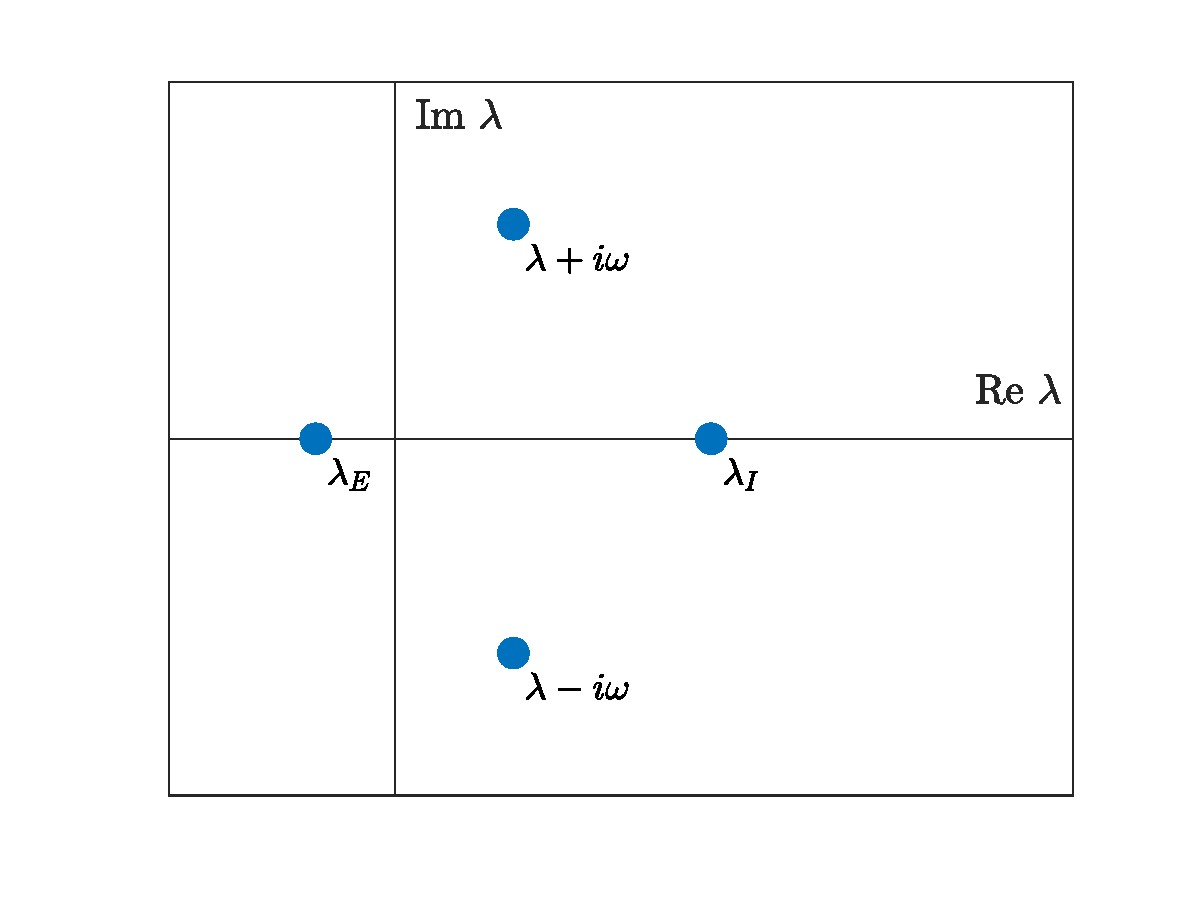
\includegraphics[width=7cm]{images/eigpattern1.eps} &
    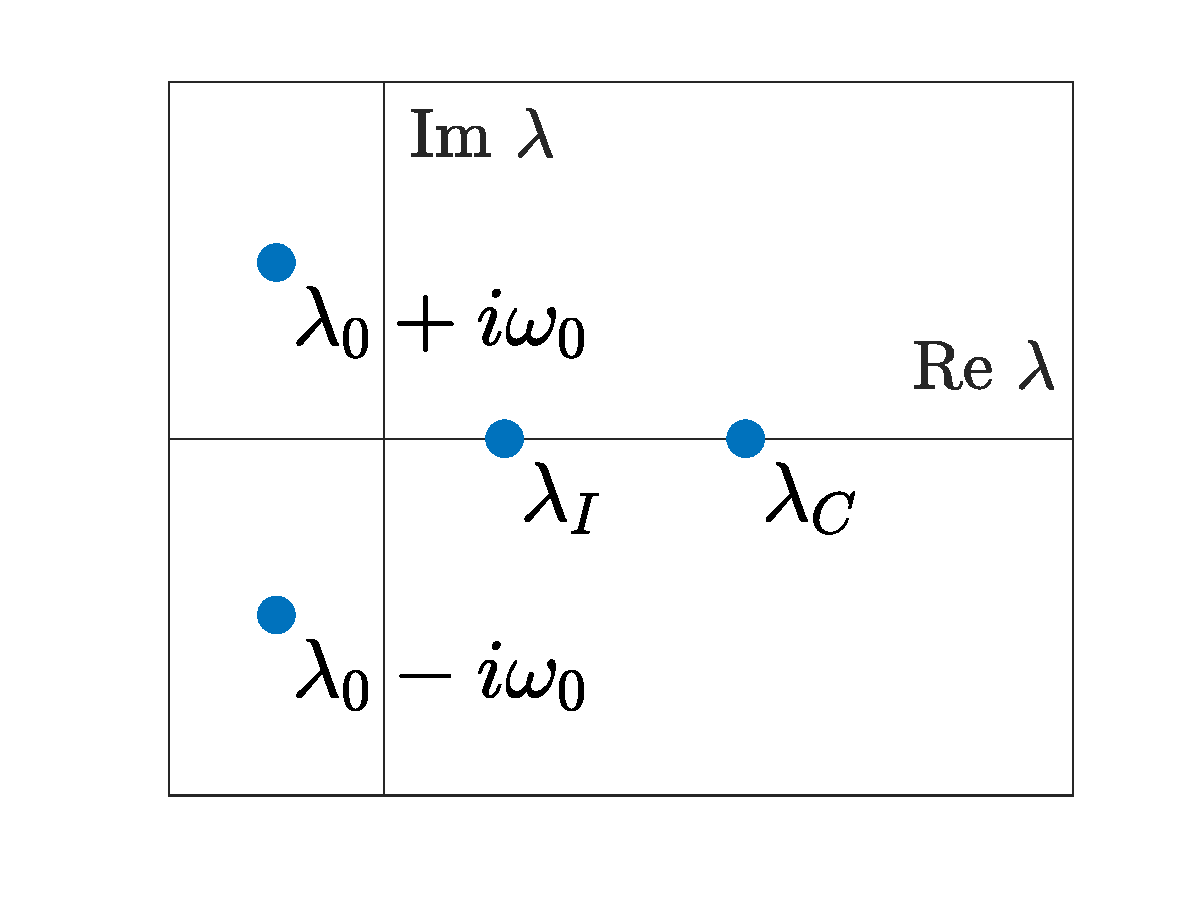
\includegraphics[width=7cm]{images/eigpattern2.eps} \\
    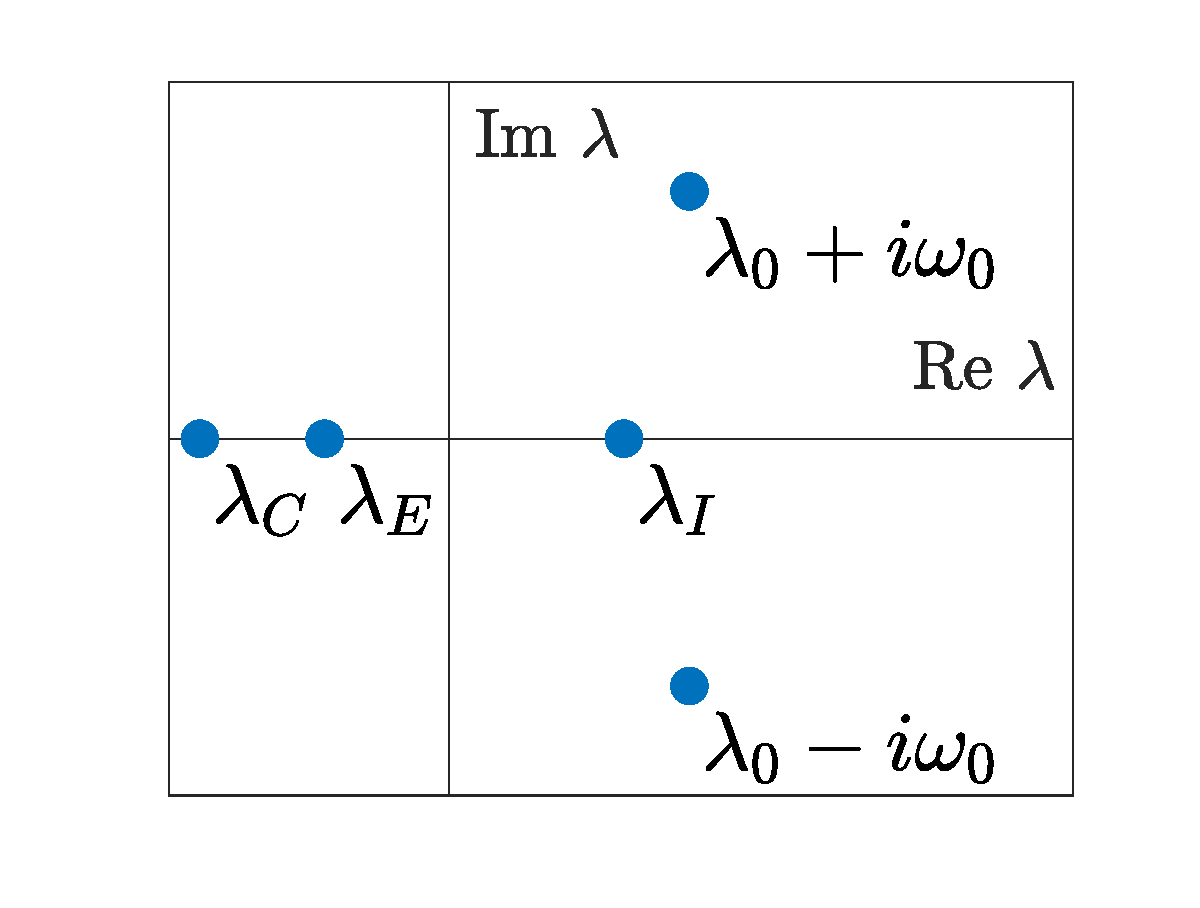
\includegraphics[width=7cm]{images/eigpattern3.eps} &
    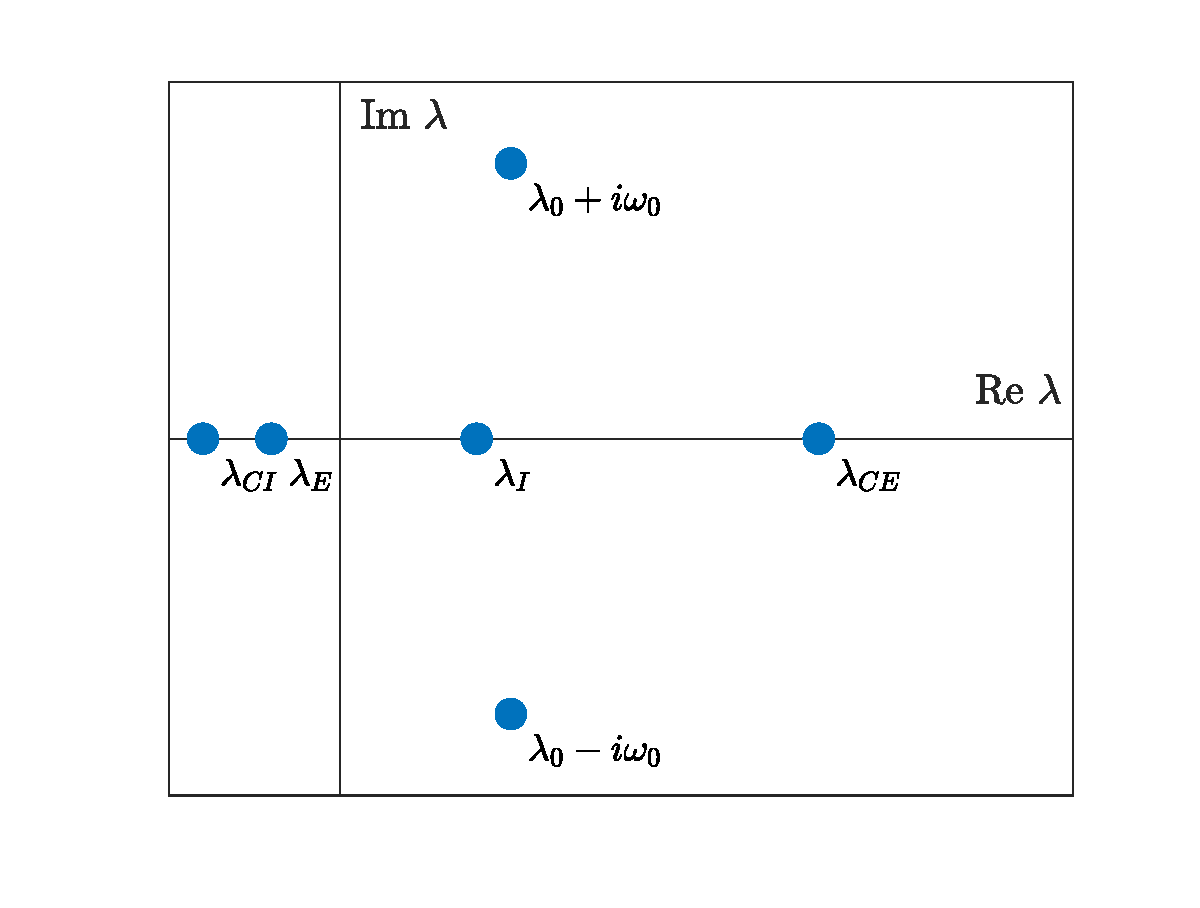
\includegraphics[width=7cm]{images/eigpattern4.eps} 
    \end{tabular}
    \caption{Eigenvalue pattern of connectivity matrix $H$ for single excitatory and single inhibitory cluster (top left), multiple excitatory clusters and single inhibitory cluster (top right), single excitatory cluster and multiple inhibitory clusters (bottom left), and multiple excitatory and inhibitory clusters (bottom right). }
    \label{fig:Heigpattern}
\end{figure}

We first reported on this phenomenon in \cite{Barreiro2017}, where we analyzed all-to-all connected, balanced excitatory-inhibitory networks. In this paper, we first flesh out some details about that system (say more). We then extend the analysis to several families of networks, which share...

\section{Model simplification}

Since we are interested in locating fixed points and periodic orbits, we can simplify the model by using the fact that all excitatory cells within each cluster must be synchronized at a fixed point or periodic orbit. In the case where there is a single excitatory cluster, if $x_1$ and $x_2$ are the activities of two excitatory cells, then it follows from \cite{Barreiro2017} that
\begin{align}\label{eq:dt_x1t2diff}
\frac{d}{dt}|x_1 - x_2|^2 \leq -2 |x_1 - x_2 |^2.
\end{align}
The only way this can be true for a fixed point (for which $\frac{d}{dt} |x_1 - x_2|^2 =0$) or for a periodic orbit (for which $x_1(t)-x_2(t) = x_1(t+T)-x_2(t+T)$ for some period $T$) is if $x_1(t) = x_2(t)$ for all $t$. If $x_1$ and $x_2$ are the activities of two cells in the same excitatory cluster, equation \cref{eq:dt_x1t2diff} holds by the same argument as in \cite{Barreiro2017}, since both neurons receive the same incoming connections with the same weights. 

For the case where there is a single cluster of inhibitory cells ($n_{CI} = 1$), if there are $n_C$ excitatory clusters containing $p$ cells each, and $n_I$ inhibitory cells ($N = pN_c + N_i$ total cells), equation \cref{eqn:sys_Basic} then reduces to the system of $n_C + n_I$ equations
\begin{equation}\label{eq:reducedsystem}
\begin{aligned}
\dot{x}_{Ej} &= -x_{Ej} + \frac{(p-1)}{\sqrt{N}}\mu_{EE} \tanh(g x_{Ej}) + \frac{1}{\sqrt{N}} \mu_{EI} \sum_k \tanh(g x_{Ik}) && j = 1, \dots, n_C \\
\dot{x}_{Ij} &= -x_{Ij} + \frac{p}{\sqrt{N}}\mu_{IE} \sum_k \tanh(g x_{Ek}) + \frac{1}{\sqrt{N}} \mu_{II} \sum_{k\neq j}  \tanh(g x_{Ik}) && j = 1, \dots, n_I
\end{aligned}
\end{equation}
$x_{Ej}$ is the activity for the excitatory cluster $j$, and $x_{Ij}$ is activity for the inhibitory cell $j$. In matrix form, equations \cref{eq:reducedsystem} can be written
\begin{equation}\label{eq:reducedmatrixform}
\dot{\xvec} = -\xvec + \frac{1}{\sqrt{N}} \tilde{H} \tanh(g \xvec),
\end{equation}
where $\xvec = (x_{E1}, \dots, x_{En_C}, x_{I1}, \dots, x_{In_I})^T$, and 
\[
\tilde{H} = \left[ \begin{array}{c|c}
    \\
    (p-1) \mu_{EE} I_{n_C} & \mu_{EI} \Onevec_{n_C \times n_I}\\
    \\
    \hline
    \\
    p \mu_{IE} \Onevec_{n_I \times n_C} & \mu_{II} \mathbf{K}_{n_I} \\
    \\
    \end{array}
    \right]
\]
For the remainder of this paper we will use $f = 0.8$ for a 4-to-1 excitatory-to-inhibitory ratio, which is typical for cortical networks [REFERENCE].
 
\section{Single excitatory and inhibitory cluster}

The simplest case (considered in \cite{Barreiro2017}) involves a single excitatory cluster and a single inhibitory cluster. The matrix $H$ reduces to
\[
H = 
\left[ \begin{array}{c|c}
\\
\mu_{EE} \Kvec_{n_E} & \mu_{EI} \Onevec_{n_E \times n_I}\\
\\
\hline
\\
\mu_{IE} \Onevec_{n_I \times n_E} & \mu_{II} \mathbf{K}_{n_I} \\
\\
\end{array}
\right]
\]
We choose the weights so that the network is \emph{balanced}; that is, the excitatory and inhibitory currents coming into each cell should approximately cancel (CITE Rajan and Abbott). To achieve this balance, we set $\mu_{EI} = -\alpha \mu_{EE}$ and $\mu_{II} = -\alpha \mu_{IE}$, where $\alpha = \frac{f}{1-f}$. For simplicity, we also take $\mu_{IE} = \mu_{EE}$. The spectrum of $H$ is now easy to compute \cite{Barreiro2017}. The eigenvalues of $H$ (top left panel of \cref{fig:Heigpattern}) are
\begin{itemize}
    \item $\lambda_I := \alpha \mu_{EE} > 0$ with multiplicity $n_I - 1$
    \item $\lambda_E := -\mu_{EE} < 0$ with multiplicity $n_E - 1$
    \item One complex pair $\lambda_0 \pm i \omega_0$, with $\lambda_0 := \mu_{EE}\frac{\alpha - 1}{2}$ and $\omega_0 := \mu_{EE}\sqrt{\alpha+1}\sqrt{n_E - \frac{\alpha+1}{4}}$. 
\end{itemize}
It is straightforward to check that $\lambda_E < 0 < \lambda_0 < \lambda_I$. The linearization about the equilibrium point $\xvec = 0$ is the constant matrix $DF(0) = \frac{g}{\sqrt{N}}H - I_n$, thus the eigenvalues of $DF(0)$ are given by $\frac{g}{\sqrt{N}}\lambda - 1$ for all eigenvalues $\lambda$ of $H$. For eigenvalues of $H$ with negative real part, the corresponding eigenvalues of $DF(0)$ will always have negative real part, irrespective of $g$. On the other hand, for eigenvalues of $H$ with positive real part, the sign of the real part of the corresponding eigenvalue of $DF(0)$ depends on the bifurcation parameter $g$. This means that all bifurcations of $\xvec = 0$ involve only the eigenvalues of $H$ with positive real part. For this specific case, the bifurcations will involve only $\lambda_I$ and $\lambda_0$.

\subsection{Bifurcations of the origin}

As the bifurcation parameter $g$ is increased from 0, the eigenvalues of $DF(0)$ corresponding to $\lambda_I$ crosses the imaginary axis at
\begin{equation}\label{eq:pitchlocation}
    g = g_0 := \frac{\sqrt{N}}{\alpha \mu_{EE}}.
\end{equation}
As $g$ is further increased, the complex pair of eigenvalues crosses the imaginary axis at 
\begin{equation}\label{eq:0hopflocation}
    g= g_H := \frac{ 2\sqrt{N} }{ (\alpha-1)\mu_{EE} }.
\end{equation}
The origin $\xvec = 0$ is a stable equilibrium for $g < g_0$, at which point it loses stability in a symmetric pitchfork bifurcation, where $n_I -1$ eigenvalues cross the imaginary axis simultaneously. 

At $g = g_H$, the origin undergoes a Hopf bifurcation. For $g > g_H$, numerical computation shows that there is a limit cycle for which all excitatory cells are synchronized and all inhibitory cells are synchronized. [THIS PART NEEDS WORK]. We can show that such a limit cycle exists for $g > g_H$ by reducing \cref{eqn:sys_Basic} to the two-dimensional system
\begin{equation}\label{eq:2dsystem}
\begin{aligned}
\dot{x} &= f(x, y) := -x + \frac{\mu_{EE}}{\sqrt{N}}\left((\alpha n_I - 1) \tanh(g x) - \alpha n_I \tanh(g y) \right) \\
\dot{y} &= g(x, y) := -y + \frac{\mu_{EE}}{\sqrt{N}}\left( \alpha n_I \tanh(g x) - \alpha (n_I - 1) \tanh(g y) \right), 
\end{aligned}
\end{equation}
where $x$ represents the synchronized excitatory cell activity and $y$ represents the synchronized inhibitory cell activity, and we used $n_E = \alpha n_I$. Since $-1 < \tanh x < 1$, we can solve $f(x, y) = 0$ for $y$ in terms of $x$ when $|x| < 2 n_E -1$ to get
\[
x = 
\]

First, we note that the origin is the only fixed point of this system for all $N$ and all $g > 0$. \textbf{(This may be difficult to show analytically)}.  Figure \ref{fig:nullclines} shows the $x$ and $y$ nullclines (the surfaces where $\dot{x} = 0$ and $\dot{y} = 0$, respectively) for \cref{eq:2dsystem}. \textbf{(This should look qualitatively the same for all values of $N$ and $g > 0$)}. 
The only intersection point of the nullclines is at the origin. Linearizing about the origin, there is a single complex pair of eigenvalues which crosses the imaginary axis at $g = g_H$, given by \cref{eq:0hopflocation}. For $g > g_H$, the origin is an unstable fixed point. To show there is a limit cycle for $g > g_H$, we use the Poincare-Bendixson theorem. We draw a square around the origin with corners $(-a, -a)$ and $(a, a)$. On the line $x = a$, for $a$ large, 
\[
\dot{x} \leq -a + \frac{2 n_E}{\sqrt{N}} = -a + 2 f \sqrt{N},
\]
which can be made negative by taking $a$ sufficiently large. Similarly, we can take $a$ sufficiently large so that the vector field defined by Fig. \ref{eq:2dsystem} points inward at all points on the square (see right panel of \cref{fig:nullclines}). Since the origin is repelling for $g > g_H$, it follows from the Poincare-Bendixson theorem that there is a limit cycle surrounding the origin for $g > g_H$. Although we note that this limit cycle is stable for the system \cref{eq:2dsystem}, the theorem says nothing about its stability in the larger system \cref{eq:reducedsystem}.

\begin{figure}
    \centering
    \begin{tabular}{cc}
    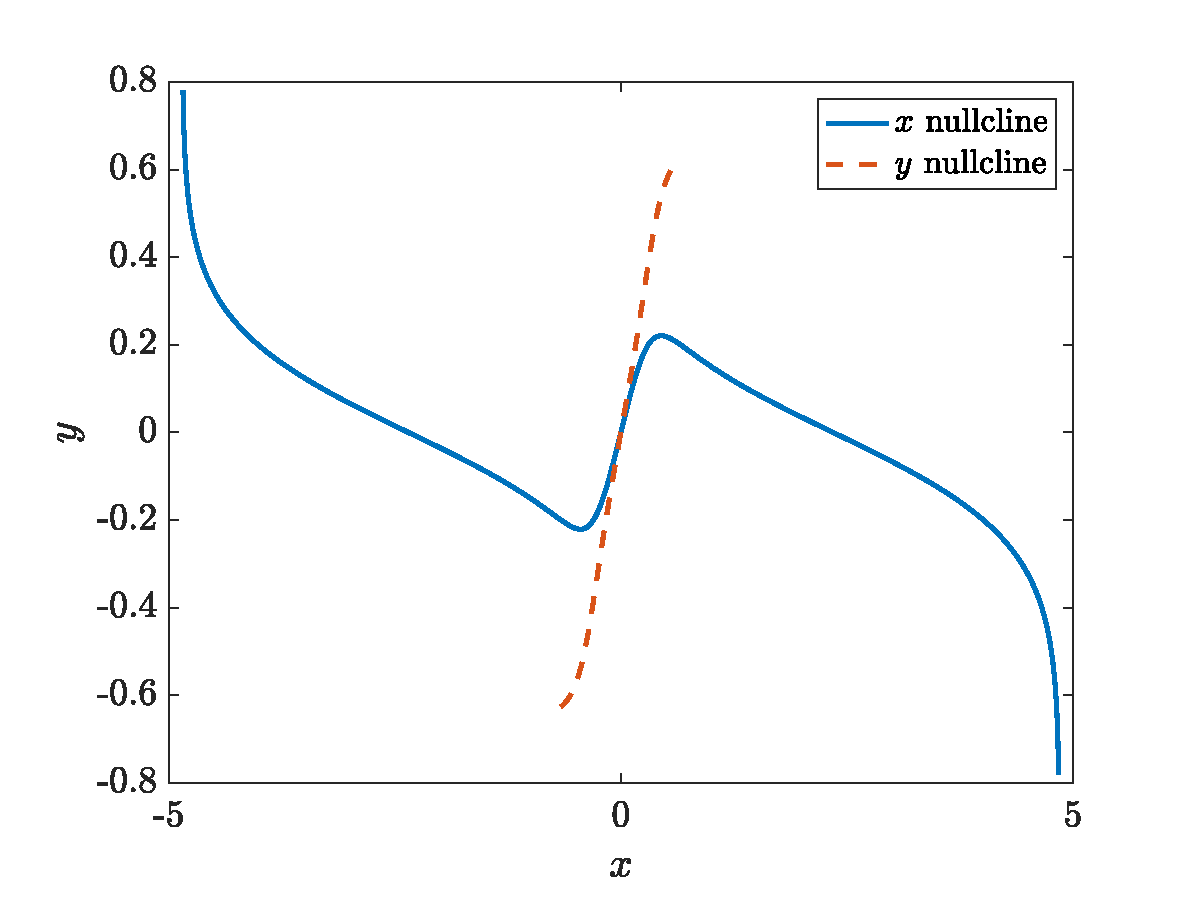
\includegraphics[width=8cm]{images/nullclines.eps} &
    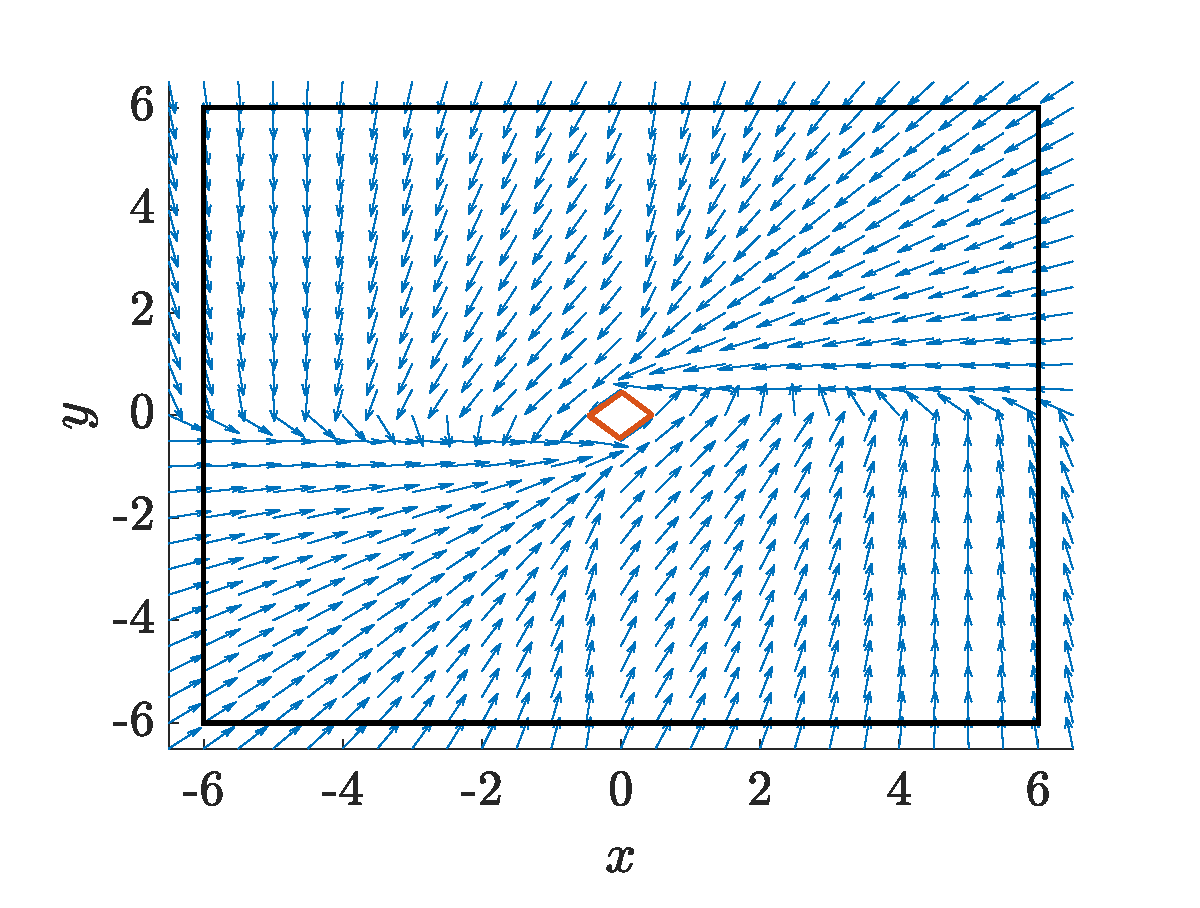
\includegraphics[width=8cm]{images/trappingregion.eps}
    \end{tabular}
    \caption{Left panel shows $x$ and $y$ nullclines for the system \cref{eq:2dsystem}. Right panel shows the slope fields for \cref{eq:2dsystem}. Slope field point inward on black box. Small limit cycle visible in center of figure. $N = 20$, $g = 5$, $\alpha = 4$, and $\mu_{EE} = 0.7$.}
    \label{fig:nullclines}
\end{figure}


\subsection{Solutions after symmetric pitchfork bifurcation}
These solutions merit some discussion, because this is where symmetry comes into play.  Our main tool is the \emph{Equivariant Branching Lemma}, which tells us what type of solutions to \cref{eqn:sys_Basic} will arise at bifurcation points, when symmetries are present \cites{MR631456,GSS88Vol2,HoyleRebeccaB2006Pf:a}. Before stating this result, we introduce some terminology. Let $\Gamma$ be a finite group acting on $\mathbb{R}^N$; then we say that a mapping $F: \mathbb{R}^N  \rightarrow \mathbb{R}^N$ is \textit{$\Gamma$-equivariant} if $F(\gamma \xvec) = \gamma F(\xvec)$, for all $\xvec \in \mathbb{R}^N$ and $\gamma \in \Gamma$.  A one-parameter family of mappings $F: \mathbb{R}^N \times \mathbb{R}  \rightarrow \mathbb{R}^N$ is \textit{$\Gamma$-equivariant}, if it is $\Gamma$-equivariant for each value of its second argument.

We say that $V$, a subspace of $\mathbb{R}^N$,  is \textit{$\Gamma$-invariant} if $\gamma \vvec \in V$, for any $\vvec$ and $\gamma \in \Gamma$. We furthermore say that the action of $\Gamma$ on $V$ is \textit{irreducible} if $V$ has no proper invariant subspaces; i.e. the only $\Gamma$-invariant subspaces of $V$ are $\{0\}$ and $V$ itself. 

For a group $\Gamma$ and a vector space $V$, we define the \textit{fixed-point subspace} for $\Gamma$, denoted $\rm{Fix} (\Gamma)$, to be all points in $V$ that are unchanged under any of the members of $\Gamma$; i.e. $\rm{Fix} (\Gamma) = \{ \xvec \in V : \gamma \xvec = \xvec, \forall \gamma \in \Gamma \}$. 
%\Acomment{Note that isotropy subgroup has two meanings: check that I am correct about this} 
The \textit{isotropy subgroup of $\xvec \in V$}, denoted $\Sigma_x$, is the set of all members of $\Gamma$ under which $\xvec$ is fixed; i.e. $\Sigma_x = \{ \gamma \in \Gamma : \gamma \xvec = \xvec \}$ (we then say that a subgroup $\Sigma$ is \textit{an} isotropy subgroup of $\Gamma$, if it is the isotropy subgroup, $\Sigma_x$, for some $\xvec \in V$.)\\

Suppose we have a one-parameter family of mappings, $F(\xvec, g)$, and we wish to solve $F(\xvec, g)=0$. 
For any $(\xvec, g) \in \mathbb{R}^n \times \mathbb{R}$, let $(dF)_{\xvec,g}$ denote the $N \times N$ Jacobian matrix 
\[ \left( \frac{\partial F_j}{\partial x_k} (\xvec, g) \right)_{j, k=1...N}
\] 
A bifurcation will occur when the Jacobian ceases to be invertible --- when $(dF)_{\xvec,g}$ has a nontrivial kernel. For a $\Gamma$-equivariant mapping --- i.e. $F(\xvec,g)$ is $\Gamma$-equivariant for any value of the parameter $g$ --- we may have \textit{multiple} eigenvalues go through zero at once, because of symmetries; however, the structural changes that occur are qualitatively the same as those that occur in a non-symmetric system, with a single zero eigenvalue. 
Furthermore, we will have \textit{multiple} such solution branches, each corresponding to a subgroup of the original symmetries.  The following Lemma formalizes this fact:

%Then the Implicit Function Theorem states that we can continue to track a unique solution branch as a function of $g$, as long as the Jacobian remains invertible. When this ceases to be true --- when $(dF)_{\xvec,g}$ has a nontrivial kernel --- we have the possibility for a bifurcation. At this point the number of zero eigenvalues (whether there are one, or two, etc..) and a menagerie of further conditions will determine the qualitative properties of the structural change that occurs.
%that is $\rm{det} dF \not= 0$, where $dF_{jk} = \left( \frac{\partial F_j}{\partial x_k} \right)  It states conditions for 

%What complicates this situation for $\Gamma$-equivariant mappings --- i.e. $F(\xvec,g)$ is $\Gamma$-equivariant for any value of the parameter $g$ --- is that because of symmetries, \textit{multiple} eigenvalues will go through zero at once; however, the structural changes that occur are qualitatively the same as those that occur in a non-symmetric system, with a single zero eigenvalue. What changes is that we now have \textit{multiple} such solution branches, each corresponding to a subgroup of the original symmetries.  The following Lemma formalizes this fact:\\


\begin{thm} (Equivariant Branching Lemma: paraphrased from \cite{GSS88Vol2}, pg. 82, see also pg. 67-69 ): Let $F: \mathbb{R}^N \times \mathbb{R} \rightarrow \mathbb{R}^N$ be a one-parameter family of $\Gamma$-equivariant mappings with $F(\xvec_0, g_0) = \Zerovec$. Suppose that $(\xvec_0, g_0)$ is a bifurcation point and that, defining $V = \ker(dF)_{\xvec_0, g_0}$, $\Gamma$ acts absolutely irreducibly on $V$. Let $\Sigma$ be an isotropy subgroup of $\Gamma$ satisfying 
\begin{eqnarray}
\rm{dim}\; \rm{Fix} (\Sigma) = 1,
\end{eqnarray}
where $\rm{Fix (\Sigma)}$ is the \emph{fixed-point subspace} of $\Sigma$: that is, $\rm{Fix} (\Sigma) \equiv \{ x \in V \mid \sigma x = x, \;  \forall \sigma \in \Sigma \}$. Then there exists a unique smooth solution branch to $F = 0$ such that the isotropy subgroup of each solution is $\Sigma$. \\
\end{thm}

The reader can readily check that the right-hand side of Eqn. \eqref{eqn:sys_Basic} is $\Gamma$-equivariant, for $\Gamma = S_{n_E} \times S_{n_I}$, where $S_n$ is the group of permutations on $n$ objects. That is, we can permute the labels on the excitatory cells, and/or the labels on the inhibitory cells, without changing the equations.

At $g=g_0$, $n_I -1$ eigenvalues pass through zero: the corresponding eigenspace is the set of all zero-sum vectors with support in the inhibitory cells only; i.e. 
\[ V \equiv  \ker(dF)_{\Zerovec,g^{\ast}}  = {\rm span} \, \{ \left[  
\underbrace{\begin{matrix}0 & \cdots & 0\end{matrix}}_{n_{E}} \;
\vvec_{n_{I}} \right] \}, \qquad \vvec_{n_{I}} \perp \Onevec_{n_{I}}.\]
To check that $\Gamma$ acts irreducibly on $V$ it is sufficient to show that the subspace spanned by the \textit{orbit} of a single vector $\vvec$ (defined as the set of all values  $\gamma \vvec$, for $\gamma \in \Gamma$) is full rank; this can be readily confirmed for $\vvec_{n_{I}} = \left[ \begin{array}{ccccc} 1 & -1 & 0 & ... & 0 \end{array} \right]$, for example.   

To find the appropriate subgroup of symmetries, break the inhibitory cells up into precisely two clusters and retain only permutations within each cluster. This describes a subgroup of $\Gamma$, $\Sigma = S_{n_E} \times S_{n_{I_1}} \times S_{n_{I_2}}$, $n_{I_1} + n_{I_2} = n_I$.
Assuming that (without loss of generality) the $I_1$ neurons have the indices $n_E+1,...,n_E+n_{I_1}$, and so forth, $\Sigma$ has the fixed point subspace 
\begin{eqnarray}
\rm{Fix}(\Sigma) & = & {\rm span} \, \{ \left[  
\underbrace{\begin{matrix}0 & \cdots & 0\end{matrix}}_{n_E} \;
\underbrace{\begin{matrix}1 & \cdots & 1\end{matrix}}_{n_{I_1}} \;
\underbrace{\begin{matrix}-\frac{n_{I_1}}{n_{I_2}} & \cdots & -\frac{n_{I_1}}{n_{I_2}} \end{matrix}}_{n_{I_2}} \right] \}
\end{eqnarray}
We can check that $\rm{Fix}(\Sigma)$ is a subspace of $V$; furthermore $\dim \rm{Fix}(\Sigma) = 1$ because it can be described as the span of a single vector. 

As a consequence, there is a branch of solutions emerging at the bifurcation point $g=g_0$ for any possible division of the inhibitory cells into exactly two clusters. We refer to these as $I_1/I_2$ branches.  Each such branch may be characterized by the number $\beta = n_{I_1}/n_{I_2}$, which gives the ratio of the cluster sizes. Without loss of generality, we may take $n_{I_1} \geq n_{I_2}$, so that $\beta \geq 1$. Each cluster of inhibitory cells is synchronized.

\subsection{Solutions along $I_1/I_2$ branches}

The simplest case occurs when $n_I$ is even and $\beta = 1$, in which case $n_{I_1}=n_{I_2}$. On this branch, $x_E = 0$, and $x_{I_2} = -x_{I_1}$, i.e. there are two equally sized inhibitory populations with equal and opposite activities. Letting $x_{I_1} = x_I$, substituting these into \cref{eq:otherbranchmatrixeq}, and simplifying, we obtain the single equation (\cite{Barreiro2017}*{Eq. 16})
\[
-x_I + \frac{\alpha \mu_{EE} }{\sqrt{N}} \tanh(g x_I) = 0, 
\]
which simplifies to $\tanh(g x_I) = g_0 x_I$. Expanding the LHS in Taylor series about $g x_I = 0$,
\begin{equation}\label{eq:tanhTaylor}
g x_I - \frac{(g x_I)^3}{3} + \frac{2(g x_I)^5}{15} + \mathcal{O}\left( (g x_I)^7 \right) = g_0 x_I
\end{equation}
Keeping up to cubic terms, equation \cref{eq:tanhTaylor} simplifies to
\[
x_I \left( (g - g_0) - \frac{g^3}{3} x_I^2 \right) = 0,
\]
thus for $g$ close to $g_0$, the nonzero solution for $x_I$ is given, to leading order, by
\begin{align}\label{eq:xIapprox}
x_I &= \sqrt{ \frac{3(g - g_0) }{g^3}} && g \geq g_0.
\end{align}
We can obtain a higher-order approximation by keeping up to fifth-order terms in \cref{eq:tanhTaylor} to get
\begin{equation*}
x_I \left( (g - g_0) - \frac{g^3}{3} x_I^2 + \frac{2 g^5}{15} x_I^4 \right) = 0,
\end{equation*}
which is $x_I$ multiplied by a quadratic in $x_I^2$. To find the nonzero solution for $x_I$, we solve this quadratic for $x_I^2$ and take square roots to get, to leading order,
\begin{align}\label{eq:xIapprox5}
x_I &= \frac{1}{2} \sqrt{ \frac{5}{g^2} - \frac{\sqrt{ 5 g^5( 24 g_0 - 19 g) }}{g^5}} && g \geq g_0.
\end{align}
Comparison between the third-order approximation, the fifth-order approximation, and the numerical solution obtained by parameter continuation is shown in the left panel of \cref{fig:xIapprox}.

\begin{figure}
    \centering
    \begin{tabular}{cc}
    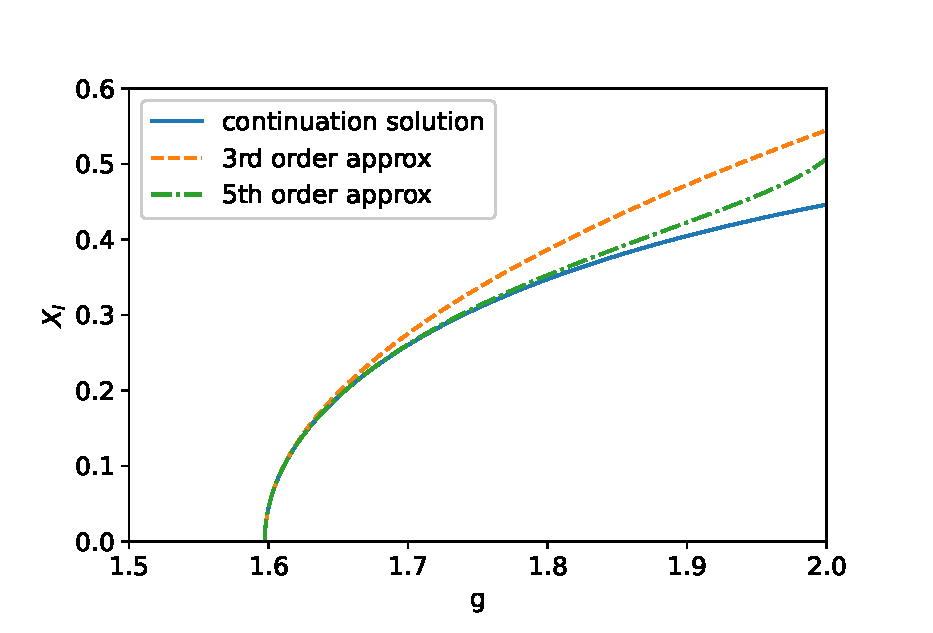
\includegraphics[width=8cm]{images/Xiapprox.eps} &
    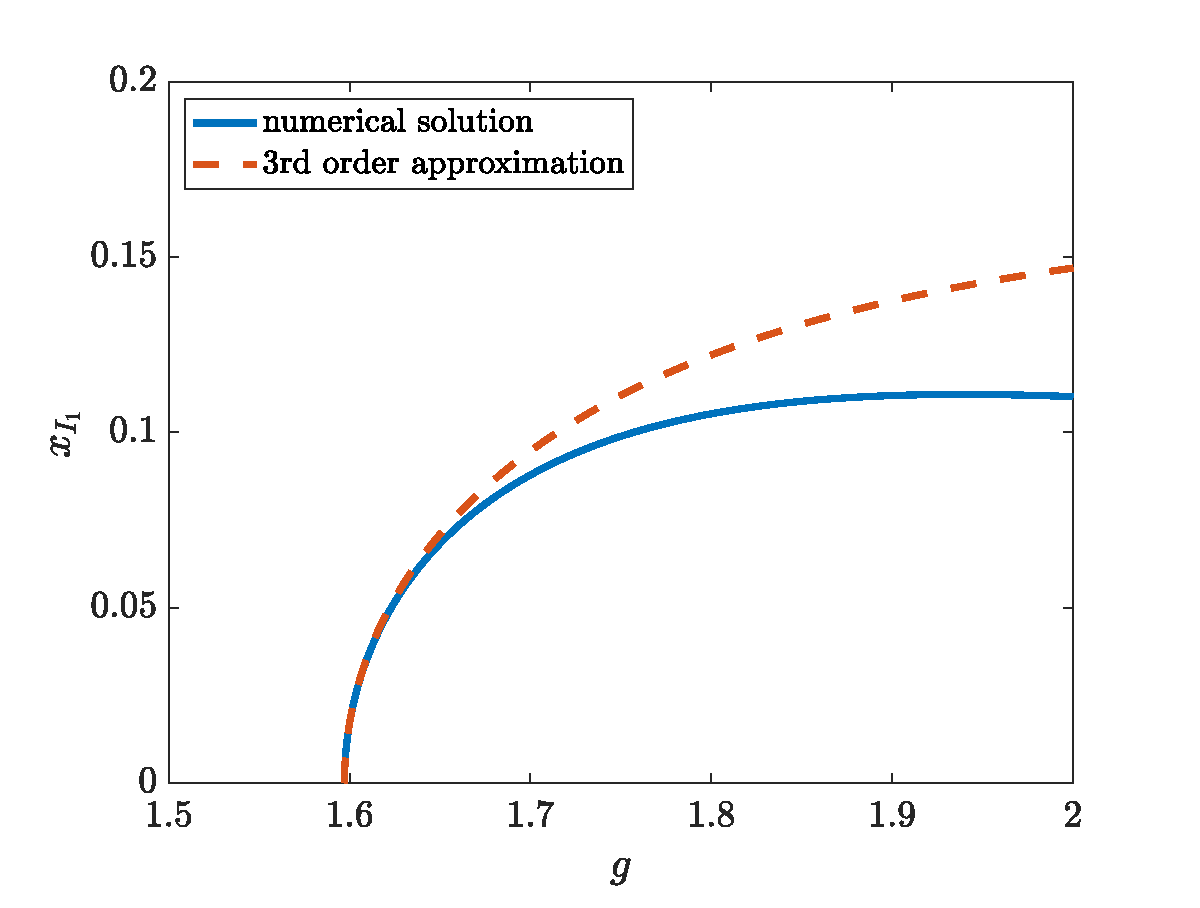
\includegraphics[width=8cm]{images/Xiapproxbeta3.eps} 
    \end{tabular}
    \caption{Third order approximation \cref    {eq:xIapprox} and fifth order approximation \cref{eq:xIapprox5} to $x_I$ on the $I_1=I_2$ branch of fixed points (left panel). Third order approximation \cref{eq:XI1} to $X_{I_1}$ on the $\beta=3$ branch (right panel). $N = 20$,  $\alpha = 4$, $\mu_{EE} = 0.7$.}
    \label{fig:xIapprox}
\end{figure}

For $\beta \neq 1$, we find the solution along each $I_1/I_2$ branch by reducing \cref{eqn:sys_Basic} to the 3-dimensional system
\begin{equation}\label{eq:otherbranchmatrixeq}
 \begin{aligned}
 \begin{bmatrix} x_E\\x_{I_1}\\x_{I_2}\end{bmatrix} 
 &= \frac{\mu_E}{\sqrt{N}} 
 \begin{bmatrix} (n_E - 1) & -\alpha \frac{\beta}{\beta+1} n_I & - \alpha \frac{1}{\beta+1} n_I  \\
 n_E  & -\alpha \left(\frac{\beta}{\beta+1} n_I-1\right) & - \alpha \frac{1}{\beta+1} n_I  \\
 n_E  & -\alpha \frac{\beta}{\beta+1} n_I & -\alpha \left(\frac{1}{\beta+1} n_I-1\right)
 \end{bmatrix}
 \begin{bmatrix} \tanh(g x_E) \\\tanh ( g x_{I_1} ) \\\tanh(g x_{I_2})\end{bmatrix},
 \end{aligned}
 \end{equation}
 where $x_E$ is the activity of the excitatory cells (which are all synchronized), and $x_{I_1}$ and $x_{I_2}$ are the activities of the two inhibitory clusters. As $N \rightarrow \infty$, numerical continuation with AUTO suggests that \cref{eq:otherbranchmatrixeq} has a solution
\begin{equation}\label{eq:I1I2asymp}
    x_{I_2} = -\beta x_{I_1} + \mathcal{O}\left( \frac{1}{N^2} \right), \quad 
    x_{I_1} = \mathcal{O}\left( \frac{1}{N} \right), \quad
     x_E = \mathcal{O}\left( \frac{1}{N^2} \right)
\end{equation}
Subtracting the second and third equations in \cref{eq:otherbranchmatrixeq}, we get
\[
 x_{I_1} - x_{I_2} = \frac{\alpha}{\mu_{EE}\sqrt{N}}\left( \tanh(g x_{I_1}) - \tanh(g x_{I_2}) \right)
 \]
Substituting \cref{eq:I1I2asymp} into this as an ansatz, expanding the $\tanh$ terms in a Taylor series to cubic order, and simplifying, we obtain the formula for $x_{I_1}$ in terms of $g$, for $g$ close to $g_0$
 \begin{align}\label{eq:XI1}
 x_{I_1} &= \sqrt{ \frac{ 3(g - g_0) }{ (1 - \beta + \beta^2 )g^3}} + \mathcal{O}\left( \frac{1}{N^2}\right)&& g \geq g_0.
\end{align}
Note that this reduces to \cref{eq:xIapprox} when $\beta = 1$. Comparison between this approximation and the numerical solution obtained by parameter continuation is shown in the right panel of \cref{fig:xIapprox}.

\begin{figure}
    \centering
    \begin{tabular}{cc}
    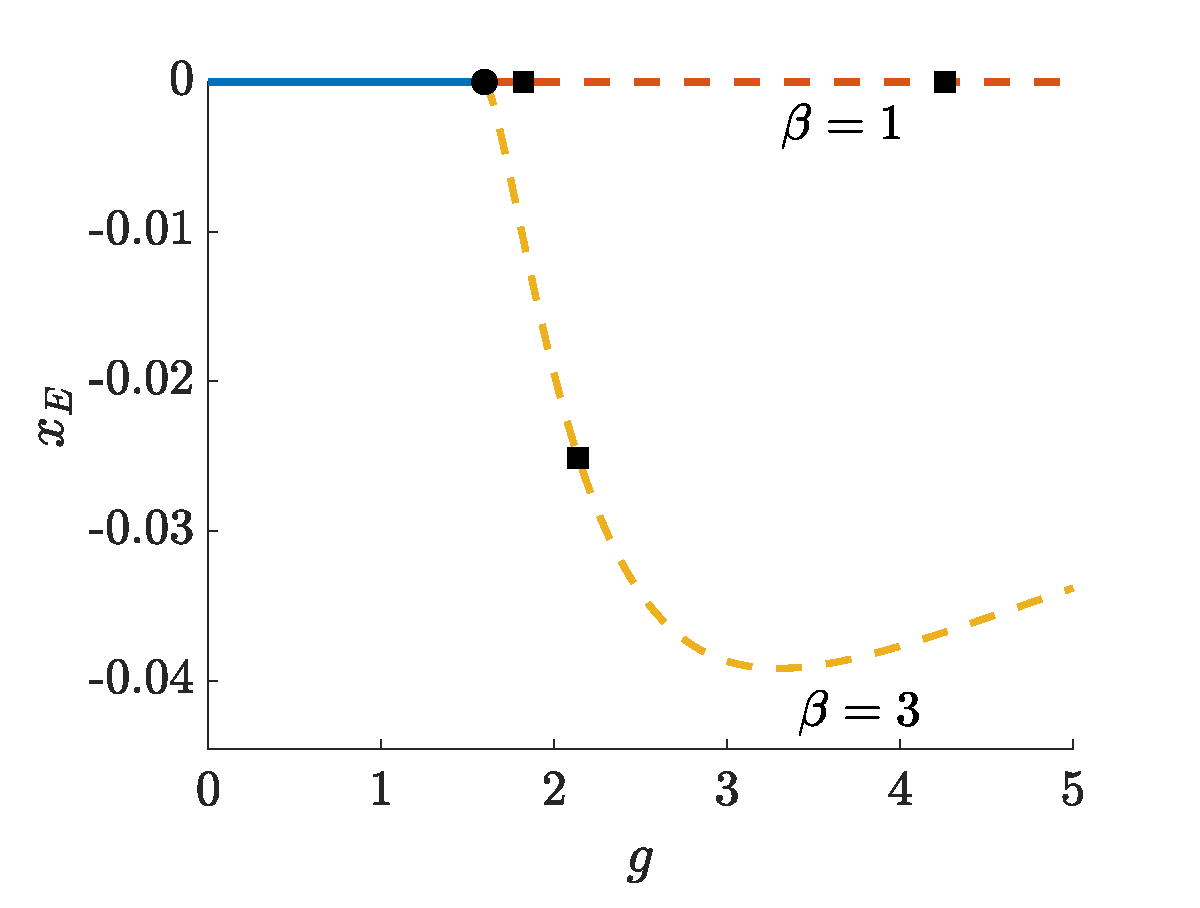
\includegraphics[width=8cm]{images/bdnoclusters20E.eps}
    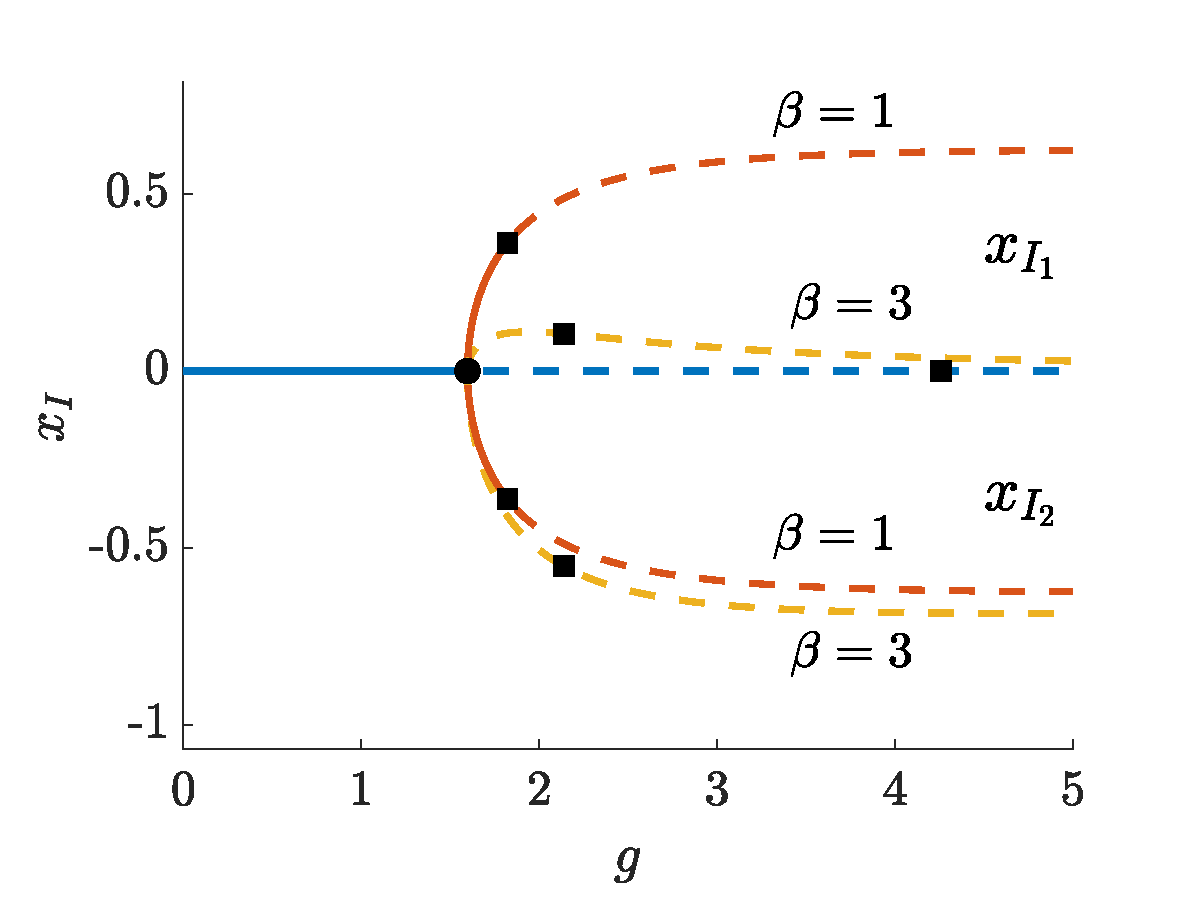
\includegraphics[width=8cm]{images/bdnoclusters20I.eps}
    \end{tabular}
    \caption{Bifurcation diagram showing both $I_1/I_2$ branches ($\beta = 1$ and $\beta = 3$) of fixed point solutions to \cref{eqn:sys_Basic}. Left panel plots $X_E$ vs $g$, right panel plots $X_{I_1}$ (above horizontal axis) and $X_{I_2}$ (below horizontal axis) vs $g$. Solid lines indicate stable fixed points, dashed lines indicate unstable fixed points. Symmetric pitchfork bifurcation at $g = g_0$ indicated with filled circle. Hopf bifurcations indicated with filled squares. 
    $N = 20$,  $\alpha = 4$, $\mu_{EE} = 0.7$.}
    \label{fig:noclusterBD1}
\end{figure}

\subsection{Hopf bifurcations on $I_1/I_2$ branches}

Along each branch of fixed points that emerges from the pitchfork bifurcation, there is a Hopf bifurcation. We can find an leading order formula for its location for large $N$. Choose any $\beta \geq 1$, and let $(x_E, x_{I_1}, x_{I_2})$ be a solution to \cref{eq:otherbranchmatrixeq} for $g > g_0$. Linearizing \cref{eq:otherbranchmatrixeq} about the fixed point branch $(x_E, x_{I_1}, x_{I_2})$, the Jacobian is:
\[
 \frac{\mu_{EE} g}{\sqrt{N}} 
 \begin{bmatrix} (n_E - 1) \sech^2(g x_E) & -\alpha \frac{\beta}{\beta+1} n_I \sech^2(g x_{I_1}) & - \alpha \frac{1}{\beta+1} n_I \sech^2(g x_{I_2}) \\
 n_E \sech^2(g x_E) & -\alpha \left(\frac{\beta}{\beta+1} n_I-1\right) \sech^2(g x_{I_1}) & -\alpha \frac{1}{\beta+1} n_I \sech^2(g x_{I_2}) \\
 n_E \sech^2(g x_E) & -\alpha \frac{\beta}{\beta+1} n_I \sech^2(g x_{I_1}) & -\alpha \left(\frac{1}{\beta+1} n_I-1 \right) \sech^2(g x_{I_2})
 \end{bmatrix} - I_3
\]
where $I_3$ is the $3 \times 3$ identity matrix. Using the Taylor expansion $\sech^2(g x) = 1 - (g x)^2 + \mathcal{O}( x^4 )$, keeping terms up to quadratic order, and substituting \cref{eq:I1I2asymp}, the Jacobian matrix above has a complex conjugate pair of eigenvalues $\lambda(g) \pm i \omega(g)$, where, to leading order,
\begin{equation}
\lambda(g) = \frac{\mu_{EE} g}{2 \sqrt{N}}\left( \alpha - 1 + \alpha \beta g^2 n_I x_{I_1}^2 \right) - 1.
\end{equation}
(This computation, and the remaining computations in this section, were performed with the aid of Wolfram Mathematica). 
When $x_{I_1} = 0$, i.e. we are linearizing about the origin, this reduces to $\lambda(g) = \frac{g}{\sqrt{N}}\lambda_0 - 1$, as required. Substituting \cref{eq:XI1} for $x_{I_1}$ gives us
\begin{equation*}
\lambda(g) = \frac{\mu_E g}{2 \sqrt{N}}\left( \alpha - 1 + \alpha \beta n_I \frac{ 3(g - g_0) }{ (1 - \beta + \beta^2 )g} \right) - 1.
\end{equation*}
To locate the Hopf bifurcation, which occurs when the complex pair of eigenvalues crosses the imaginary axis, we solve $\lambda(g) = 0$ to get
\begin{equation}\label{eq:gHbeta}
g_{H,\beta} = \frac{ 
\frac{ 3 \alpha \beta n_I }{ (1 - \beta + \beta^2 ) } g_0
+ \frac{2 \sqrt{N}}{\mu_{EE}} 
}
{
\frac{ 3 \alpha \beta n_I }{ (1 - \beta + \beta^2 ) } + \alpha - 1
}
+ \mathcal{O}\left( \frac{1}{N^{3/2}} \right)
\end{equation}
A plot of $g_{H,\beta}$ versus $N$ for various $\beta$ is given in \cref{fig:Hopfplots}. This formula, and the order of the remainder term, agrees with results from numerical parameter continuation (see \cref{fig:Hopferror}). As $N \rightarrow \infty$, which implies $n_I = f N \rightarrow \infty$, the first terms in the numerator and denominator of \cref{eq:gHbeta} dominate, thus $g_H(g) \rightarrow g_0$ as $N \rightarrow \infty$ for all $\beta$ (see \cref{fig:Hopfplots}). Substituting $g_0 = \sqrt{N}/\alpha \mu_{EE}$ and simplifying, equation \cref{eq:gHbeta} becomes
\begin{equation}\label{eq:ghopfformula}
g_{H,\beta} = 
\frac{\sqrt{N}}{\mu_{EE}} 
\frac{ 3 \beta n_I  + 2(1 - \beta + \beta^2 ) }
{ 3 \alpha \beta n_I + (\alpha - 1)(1 - \beta + \beta^2 ) }
+ \mathcal{O}\left( \frac{1}{N^{3/2}} \right)
\end{equation}
Differentiating \cref{eq:ghopfformula} with respect to $\beta$ and simplifying,
\begin{equation}\label{eq:gprime}
g_{H,\beta}' = 
    \frac{ 
    3 (\alpha+1) \left(\beta^2-1\right) n_I
    }
    {
    \left(\alpha \left(\beta^2+\beta (3 n_I -1)+1\right)-\beta^2+\beta-1\right)^2},
\end{equation}
which is 0 at $\beta = 1$ and positive for $\beta > 1$. Thus $g_{H,\beta}$ increases with $\beta$ for $\beta \geq 1$. This confirms the ordering of the Hopf bifurcations in $\beta$ seen in \cref{fig:Hopfplots}. 

\begin{figure}
    \centering
    \begin{tabular}{cc}
    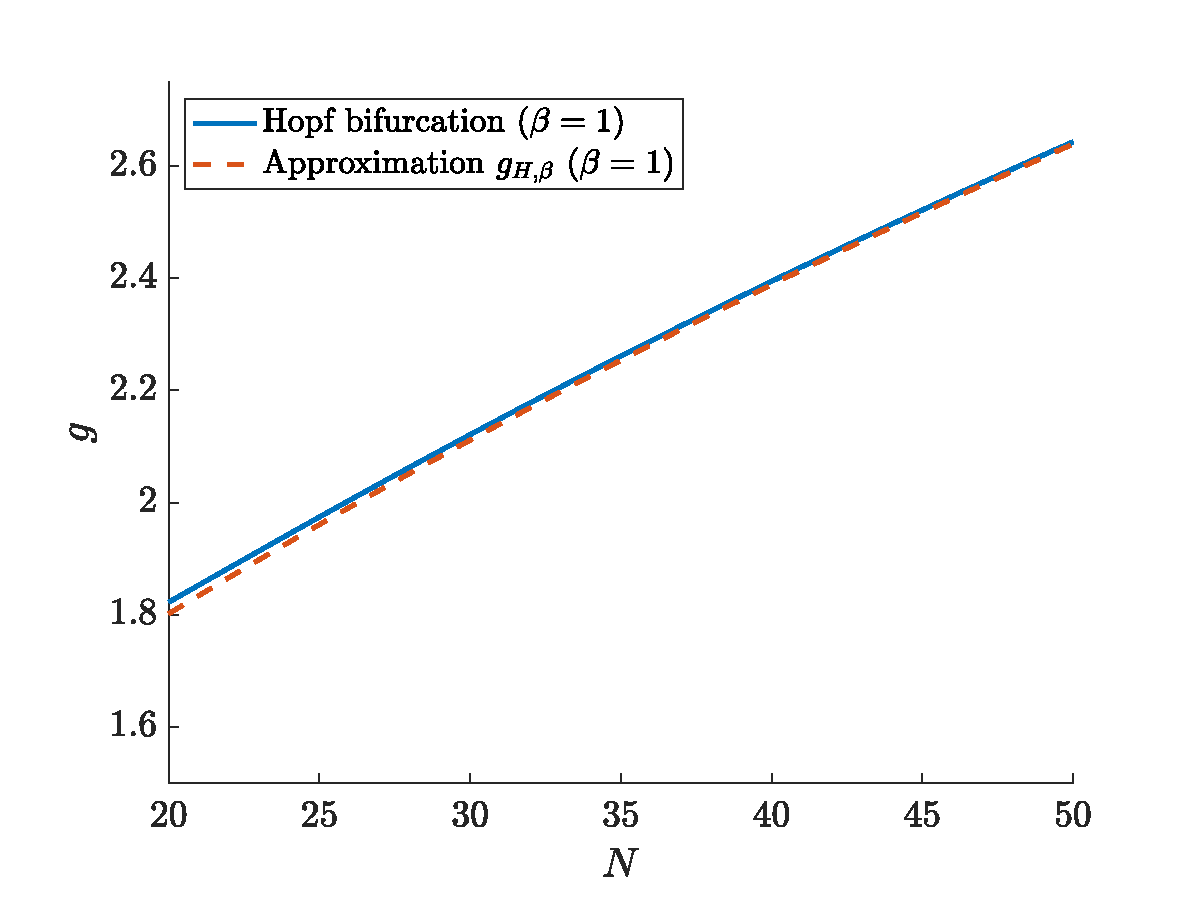
\includegraphics[width=8cm]{images/Hopfapproxbeta1.eps}
    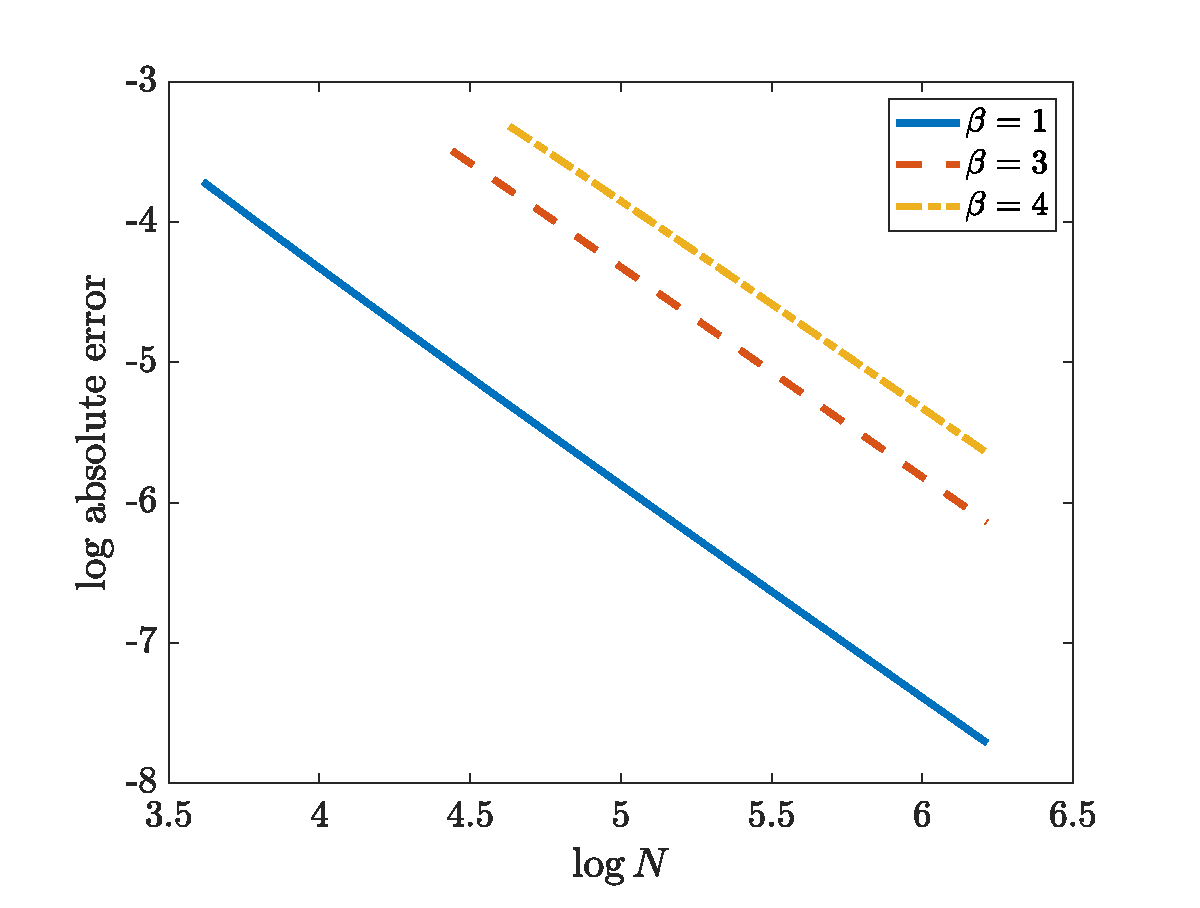
\includegraphics[width=8cm]{images/Hopfapproxerror.eps}
    \end{tabular}
    \caption{Left panel plots compares approximation \cref{eq:ghopfformula} to computed location of Hopf bifurcation for $I_1/I_2$ branch with $\beta = 1$. Right panel plots log of absolute error of approximation \cref{eq:ghopfformula} vs $\log N$ for $\beta = 1$, 3, and 4. Slope of line is approximately -1.5 for all three $\beta$. $\alpha = 4$, $\mu_{EE}= 0.7$. }
    \label{fig:Hopferror}
\end{figure}

\begin{figure}
    \centering
    \begin{tabular}{cc}
    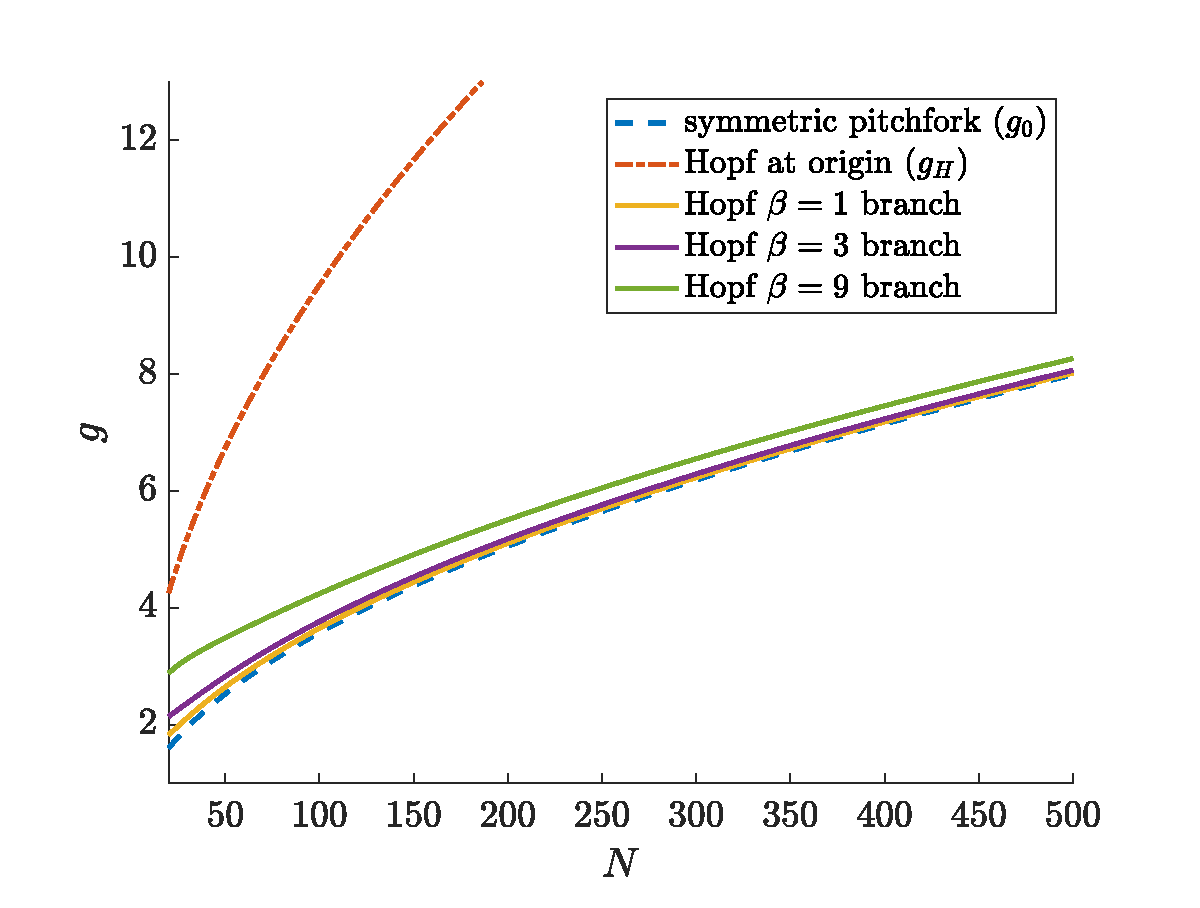
\includegraphics[width=8cm]{images/HopfNvsg.eps}
    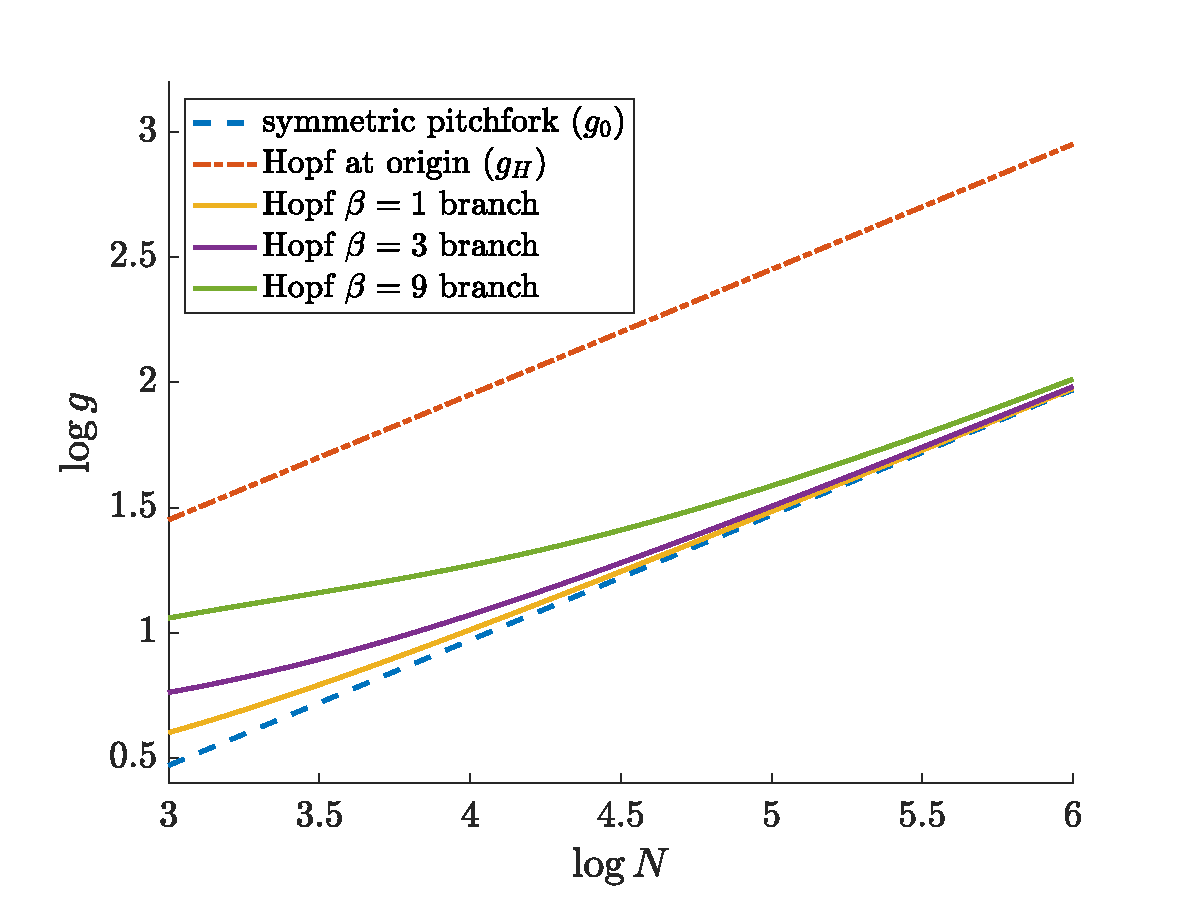
\includegraphics[width=8cm]{images/HopflogNvslogg.eps}
    \end{tabular}
    \caption{Left panel shows location in $(N, g)$ space of symmetric pitchfork bifurcation at $g_0$ (dashed line), Hopf bifurcation at origin at $g_H$ (dash-dotted line), and Hopf bifurcations on $I_1/I_2$ branches for select $\beta$ (solid lines, arranged from bottom to top in increasing $\beta$). Right panel is same data on a log-log plot.}
    \label{fig:Hopfplots}
\end{figure}
% At the Hopf bifurcation, the imaginary part of eigenvalue scales as $\sqrt{N}$, which is the frequency of oscillation of the limit cycle.

\subsection{Behavior of the $I_1/I_2$ branch for large $g$} \label{sec:stab_largeg}
We have characterized the three-cluster fixed point solutions near their origin $g=g_0$; next, we describe how they behave for large $g$. We summarize the main points here; detailed calculations can be found in an Appendix.

Defining $y_E = \tanh(gx_E)$, etc., the equations defining a fixed point are:

 \begin{align*}
        x_E &= \frac{\mu_E}{\sqrt{N}} \left[ (n_E - 1)y_E - \alpha n_{I_1} y_{I_1} - \alpha n_{I_2} y_{I_2} \right] \\
        x_{I_1} &= \frac{\mu_E}{\sqrt{N}} \left[ n_E y_E - \alpha (n_{I_1}-1) y_{I_1} - \alpha n_{I_2} y_{I_2} \right] \\
        x_{I_2} &= \frac{\mu_E}{\sqrt{N}} \left[ n_E y_E - \alpha n_{I_1} y_{I_1} - \alpha (n_{I_2}-1) y_{I_2} \right] 
    \end{align*}
or
\begin{align}
 \begin{bmatrix} x_E\\x_{I_1}\\x_{I_2}\end{bmatrix} 
 &= \frac{\mu_E}{\sqrt{N}} 
 \begin{bmatrix} (n_E - 1) & -\alpha n_{I_1} & - \alpha n_{I_2}  \\
 n_E  & -\alpha (n_{I_1}-1) & - \alpha n_{I_2}  \\
 n_E  & -\alpha n_{I_1} & - \alpha (n_{I_2}-1)  
 \end{bmatrix}
 \begin{bmatrix} y_E\\y_{I_1}\\y_{I_2}\end{bmatrix} 
 \label{eq:3cluster_solution}
 \end{align}

Using the identity $\sech^2(y) = 1-\tanh^2(y)$, the Jacobian will be
 \begin{align}
 J &= -I + 
 \frac{g\mu_E}{\sqrt{N}} 
 \begin{bmatrix} (n_E - 1) & -\alpha n_{I_1} & - \alpha n_{I_2}  \\
 n_E  & -\alpha (n_{I_1}-1) & - \alpha n_{I_2}  \\
 n_E  & -\alpha n_{I_1} & - \alpha (n_{I_2}-1)  
 \end{bmatrix}
 \begin{bmatrix} 1-y_E^2 & 0 & 0 \\0 &  1-y_{I_1}^2 & 0\\0 & 0 &1-y_{I_2}^2\end{bmatrix} 
 \label{eq:3cluster_Jac}
 \end{align}
 Note that the diagonal matrix on the right scales each column of the non-identity portion of the Jacobian. When $y_{E/I_1/I_2}=\pm 1$, its corresponding column will be zeroed out.  
 Thus when there is a solution for which all three $y_E, y_{I_1}, y_{I_2} = \pm 1$ (rather than 0), then $J=-I$ and the solution will be stable for large $g$.

Our task is facilitated by the following observations about the behavior of the $\tanh$ function; along branches for which $x_E \rightarrow \hat{x} \not= 0$, then
\[ \tanh(gx_E) \rightarrow \left\{ \begin{matrix}
    1 & \hat{x} > 0\\
    -1 & \hat{x} < 0
\end{matrix} \right.
\] 
When this is the case Eqn. \eqref{eq:3cluster_solution} becomes linear.
If $x_E \rightarrow 0$, the limiting behavior may be more complicated; if $x_E \approx \frac{\hat{x}}{g}$, then $\tanh(gx_E) \rightarrow \tanh(\hat{x}) := y_E \not= 0$.  However, we will show it is possible to solve for the limiting coordinates and thus to characterize the stability. It turns out to be most convenient to characterize solutions by the number of coordinates that have saturating non-linearities: we itemize them as $\textbf{S0}, \textbf{S1}, \cdots$ below.

\begin{enumerate}
    \item[\textbf{S3}] If $(y_E,y_{I_1},y_{I_2}) = \pm 1$, then the non-identity matrix in Eqn. \eqref{eq:3cluster_Jac} is 0 and the solution will be stable. Unfortunately, this cannot happen; there is no solution for which \textit{all} nonlinearities saturate.
    \item[\textbf{S0}] Similarly, there is no solution for which \textit{no} nonlinearity saturates; i.e. $\tanh(g x_E) \rightarrow y_E \not= \pm 1$.
    \item[\textbf{S2}] However, for $n_{I_1} = n_{I_2}$ there is a solution for which $(y_E,y_{I_1},y_{I_2}) = (0,1,-1)$; this solution is unstable. 
    \item[\textbf{S1}] For $n_{I_1}\not=n_{I_2}$, there are solutions for which one nonlinearity saturates while the other two do not.
\end{enumerate}






\begin{figure}[h]
    \centering
    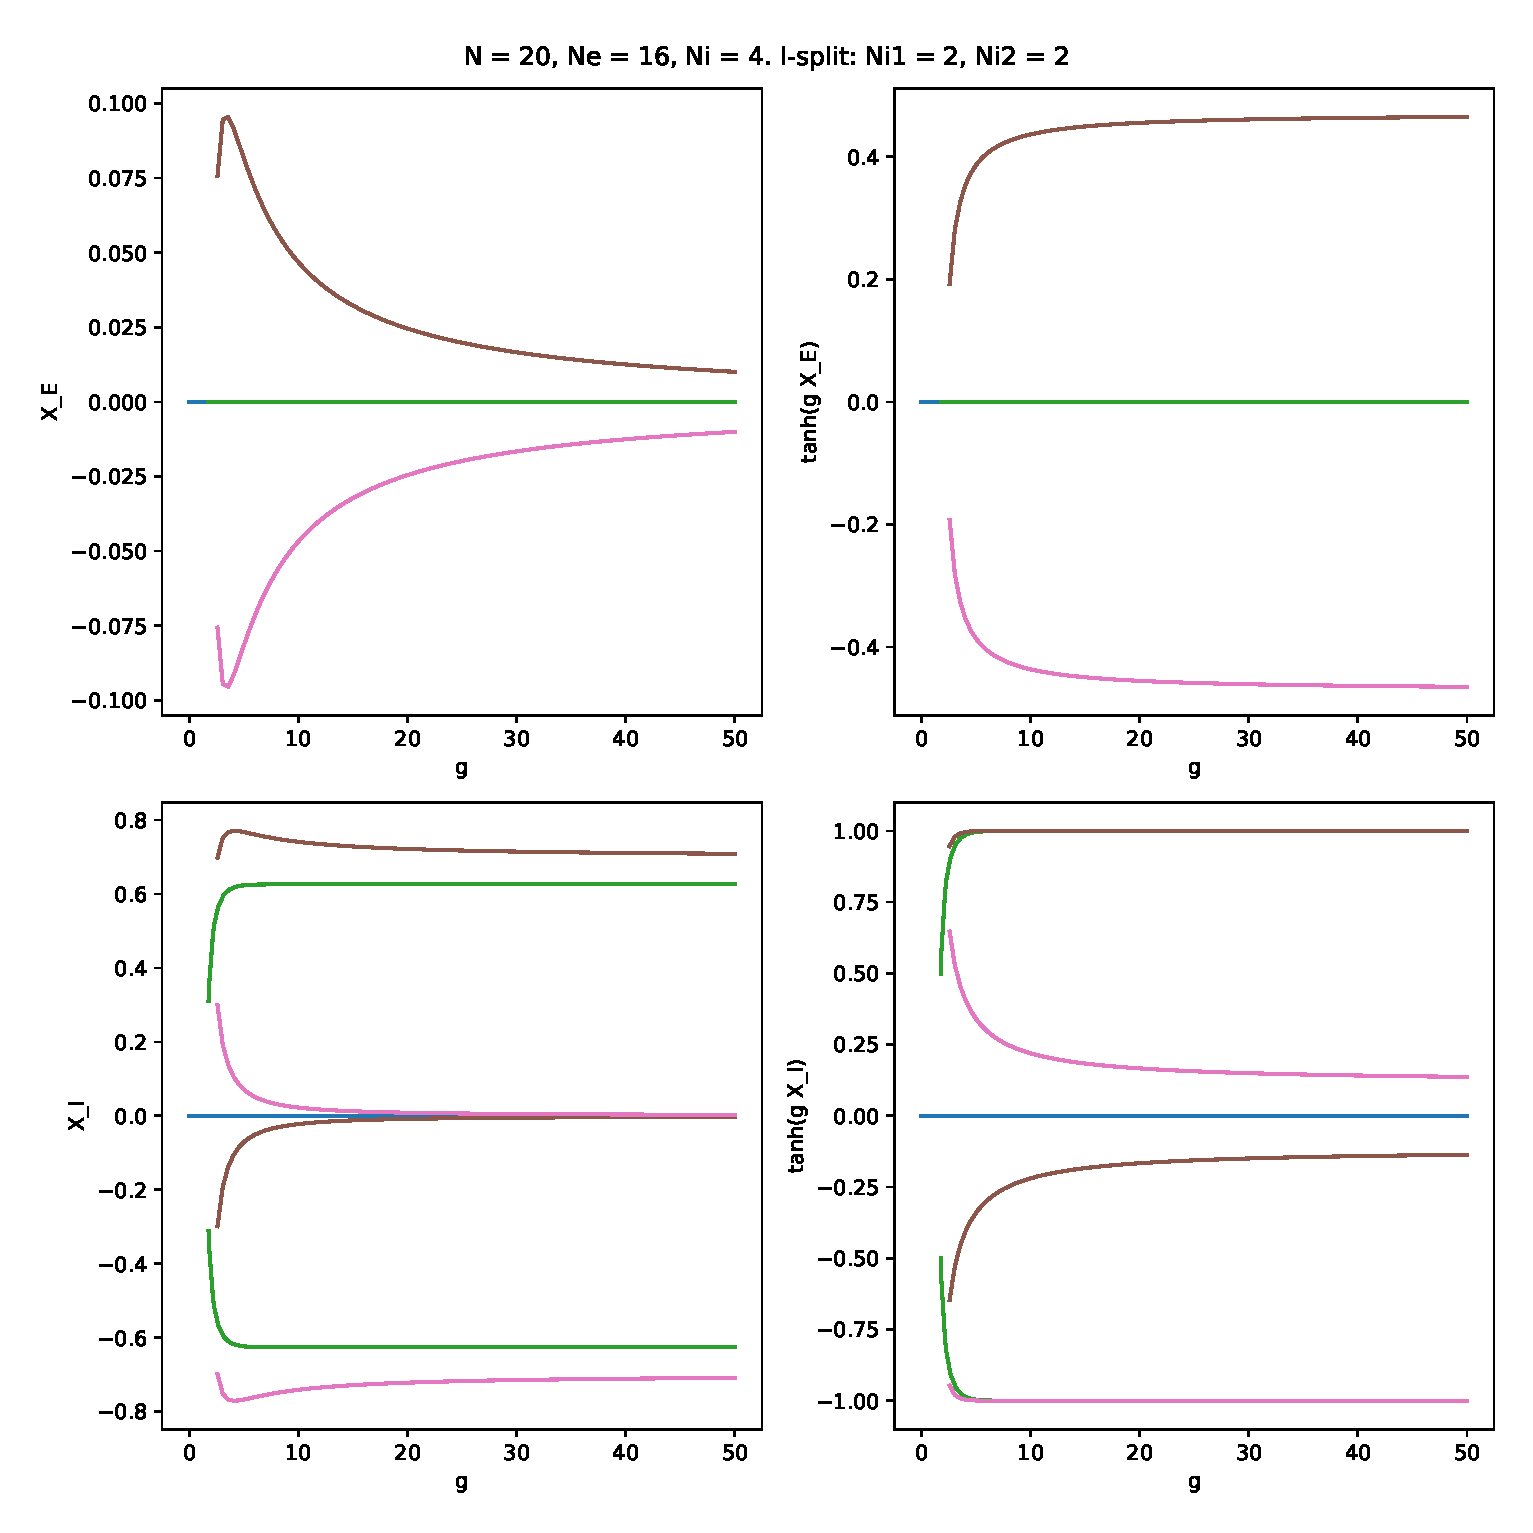
\includegraphics[width=12cm]{images/20largeg22.eps} 
    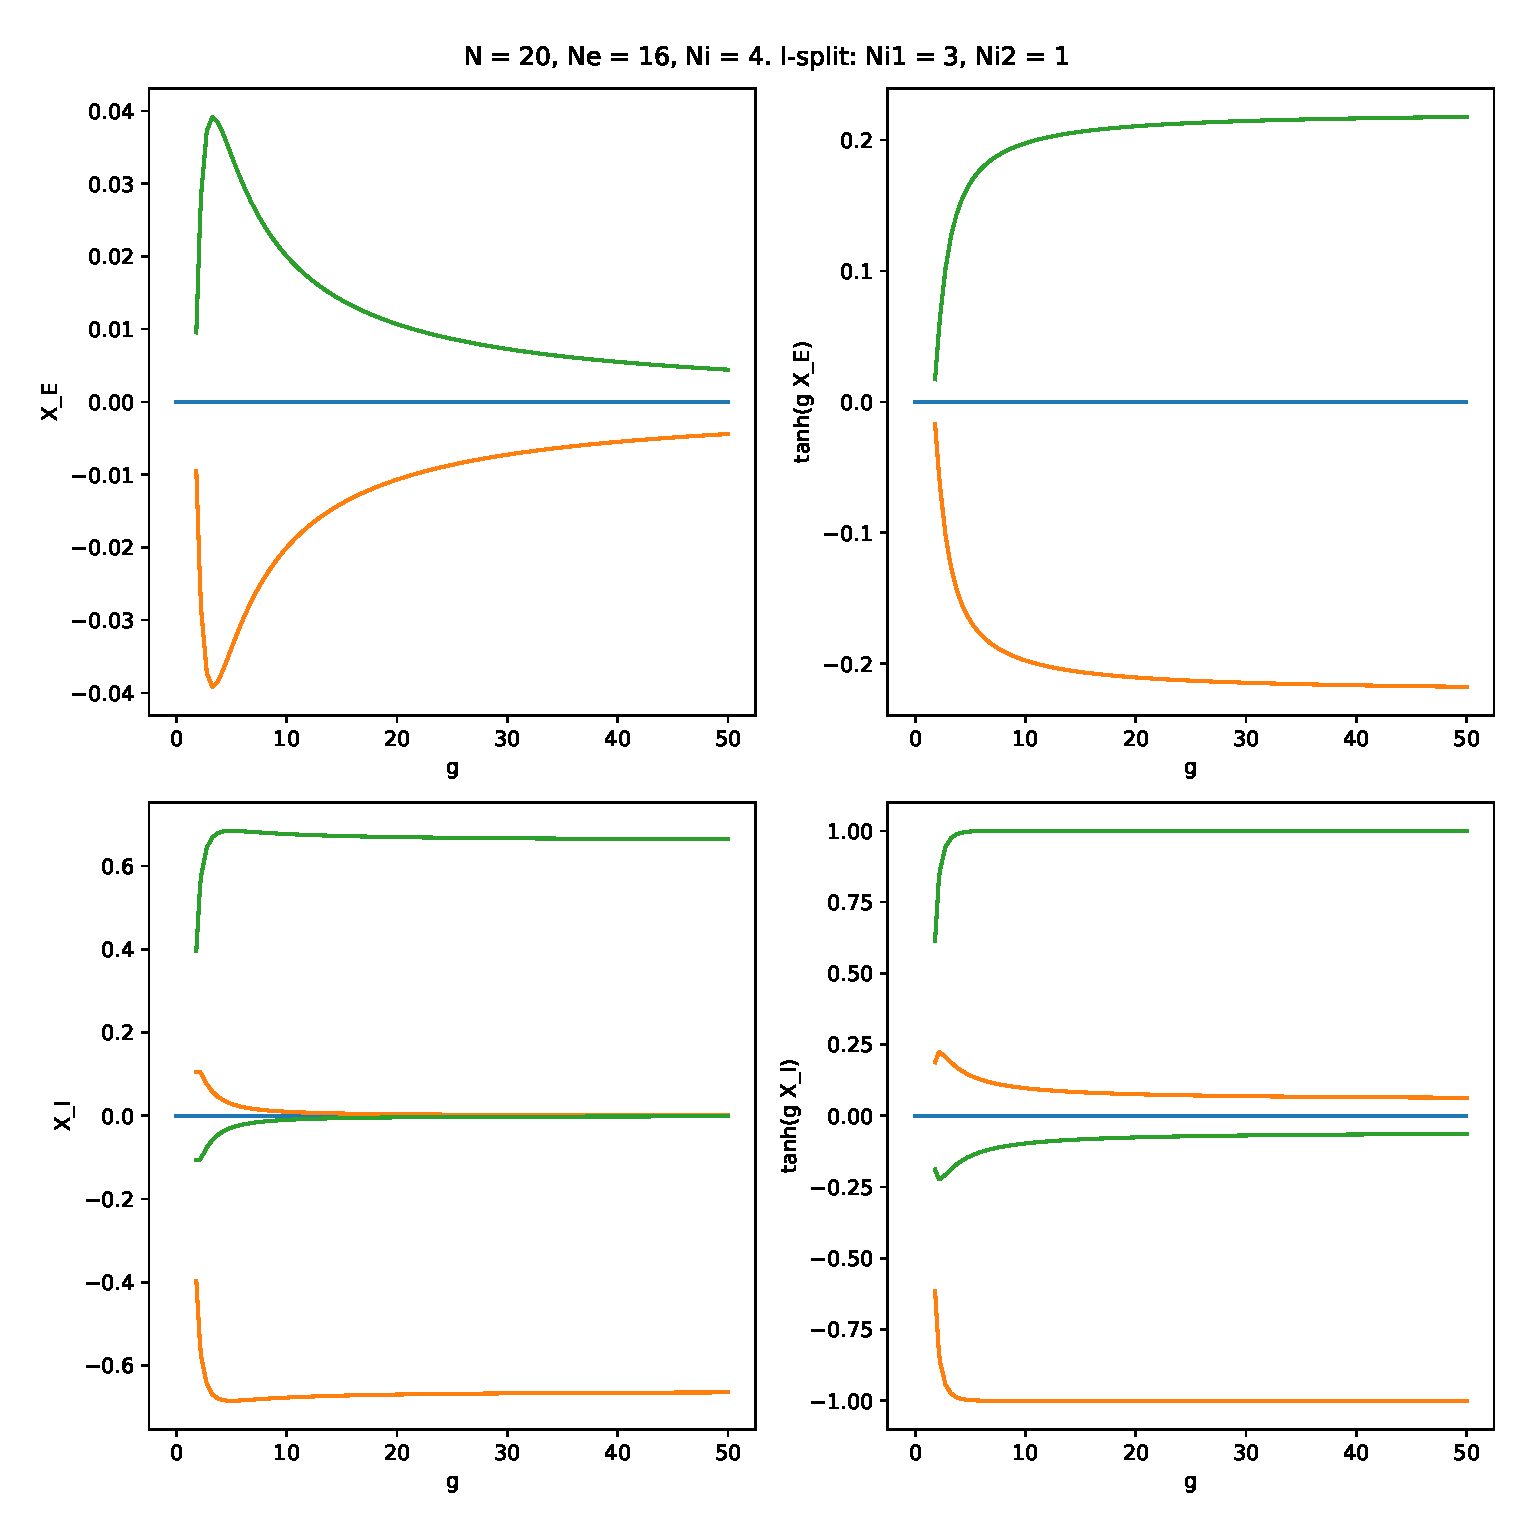
\includegraphics[width=12cm]{images/20largeg31.eps} 
    \caption{Bifurcation diagram for $N = 20$ showing 1:1 symmetry of I-cells on left, and 3:1 symmetry of I-cells on right.}
    \label{fig:20symm1}
\end{figure}


% Note that the first set of equations can be written as 
% 
% \begin{align*}
% \begin{bmatrix} x_E\\x_{I_1}\\x_{I_2}\end{bmatrix} 
% &= \frac{\mu_E}{\sqrt{N}} 
% \begin{bmatrix} -y_E + C  \\
% \alpha y_{I_1} + C  \\
% \alpha y_{I_2} + C  
% \end{bmatrix}
% \end{align*}
% where $C = \frac{\mu_E}{\sqrt{N}}\left(n_E y_E -\alpha n_{I_1} %y_{I_1} - \alpha n_{I_2} y_{I_2} \right)$.
 
 
\begin{figure}[H]
    \centering
    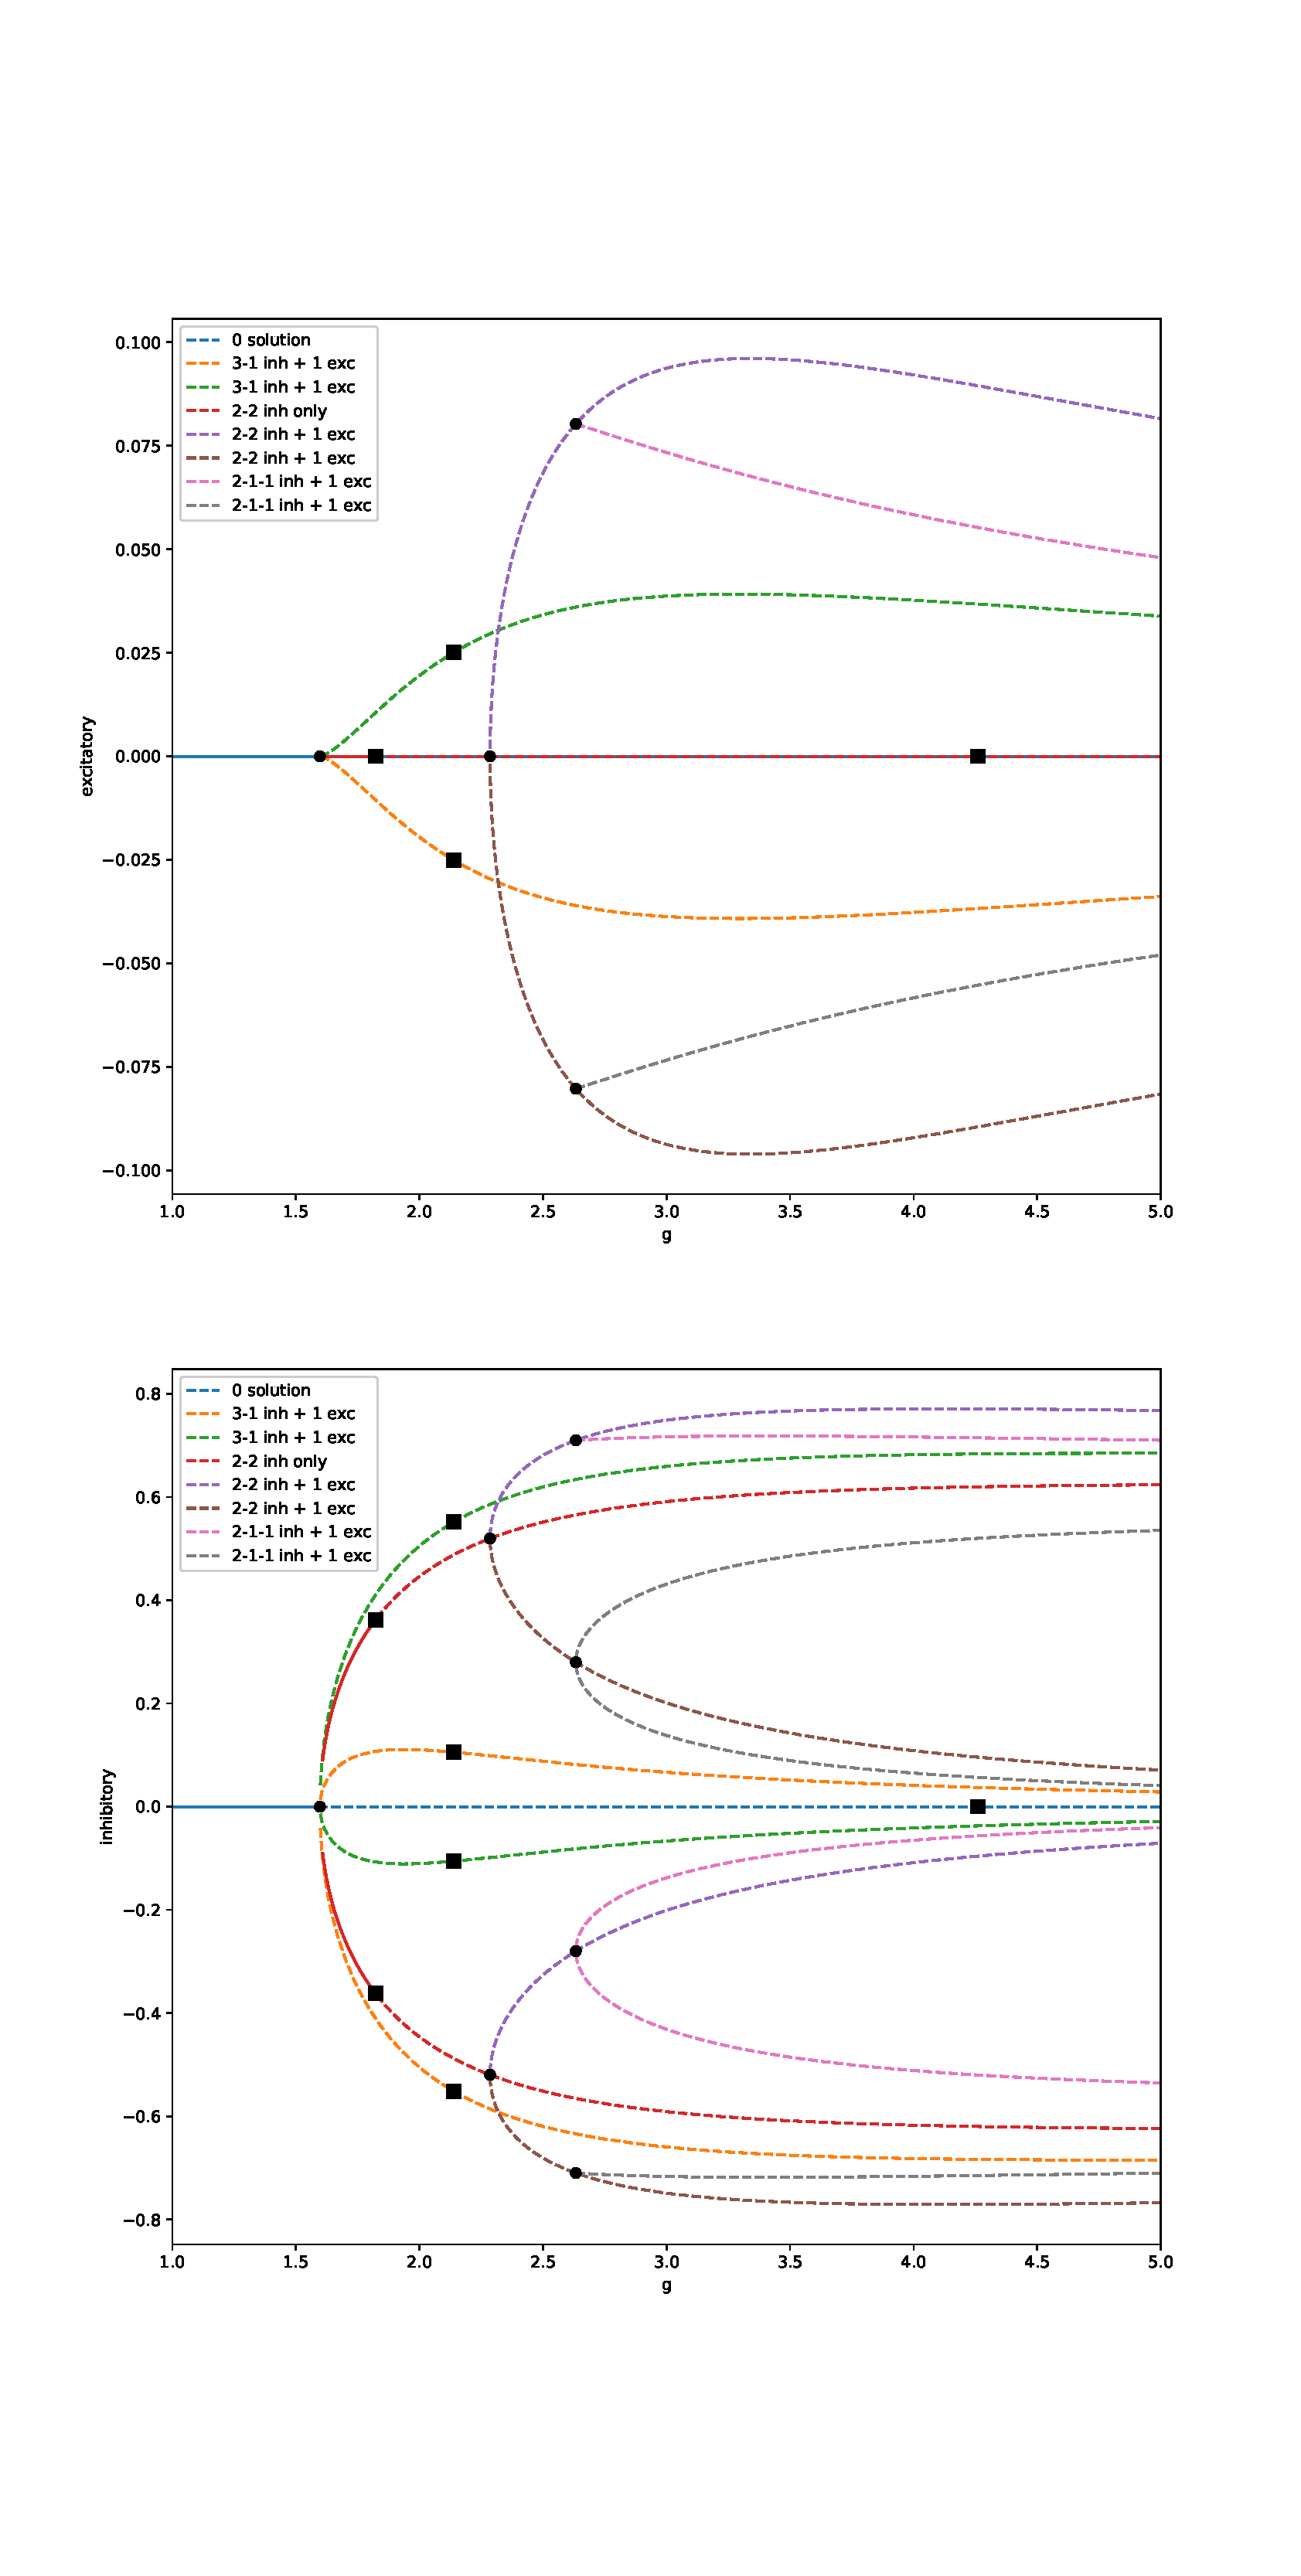
\includegraphics[width=12cm]{images/BDsingle20_E07.eps}
    \caption{Bifurcation diagram (for $\mu_{EE} = 0.7$)}
    \label{fig:20nocluster}
\end{figure}

\subsection{Periodic solutions}
We can also use AUTO to find the periodic solutions arising from the 3 Hopf bifurcations (squares in \cref{fig:20nocluster}. Below is plot of period of limit cycle vs $g$, with stable limit cycle indicated by solid line. This is identical to \cite{Barreiro2017}*{Figure 2}.

\begin{figure}[H]
    \centering
    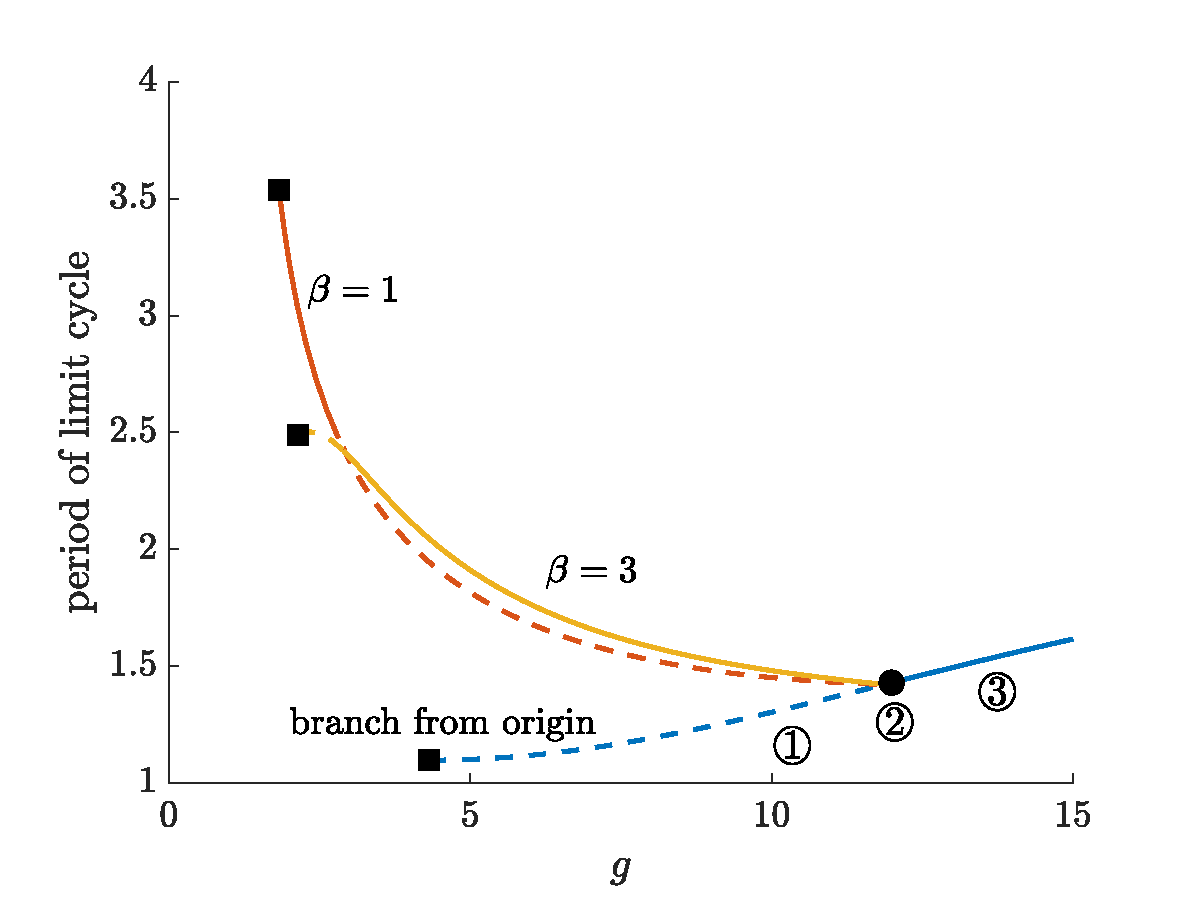
\includegraphics[width=14cm]{images/periodvsg}
    \caption{Period of limit cycle versus $g$ for periodic solutions arising from Hopf bifurcations. Stable limit cycles indicated with solid lines.}
    \label{fig:periodvsg}
\end{figure}

There is a critical value of $g$ where all the limit cycle branches come together, and after that point, there is one stable limit cycle where all the E-cells and I-cells are synchronized.
\textbf{This pattern appears to hold for all $N$.}

The plot shows location in $g$ of important points (pitchfork bifurcation, Hopf bifurcations, and point where limit cycles meet) for increasing $N$. This is done by continuing the bifurcations in a reduced three-dimensional system of one excitatory, two inhibitory populations.  
Of course, the indicated Hopf bifurcations would only occur in a real network if the ratio of inhibitory cells is valid for that particular value of $N$ (e.g. for 3:1, the total number of inhibitory cells must be a multiple of 4). The location of the pitchfork bifurcation on the zero solution is given by \cref{eq:pitchlocation}, which is confirmed on the plot below. The location of the Hopf bifurcation on the zero solution is given by \cref{eq:0hopflocation}, which is confirmed on the plot below. If the Hopf bifurcation ratio is written as $m:1$, the Hopf bifurcations appears to be ordered by increasing $m$ as $g$ increases \textbf{proof? This follows from \cref{eq:ghopfformula} and \cref{eq:gprime}}.

\begin{figure}[H]
    \centering
    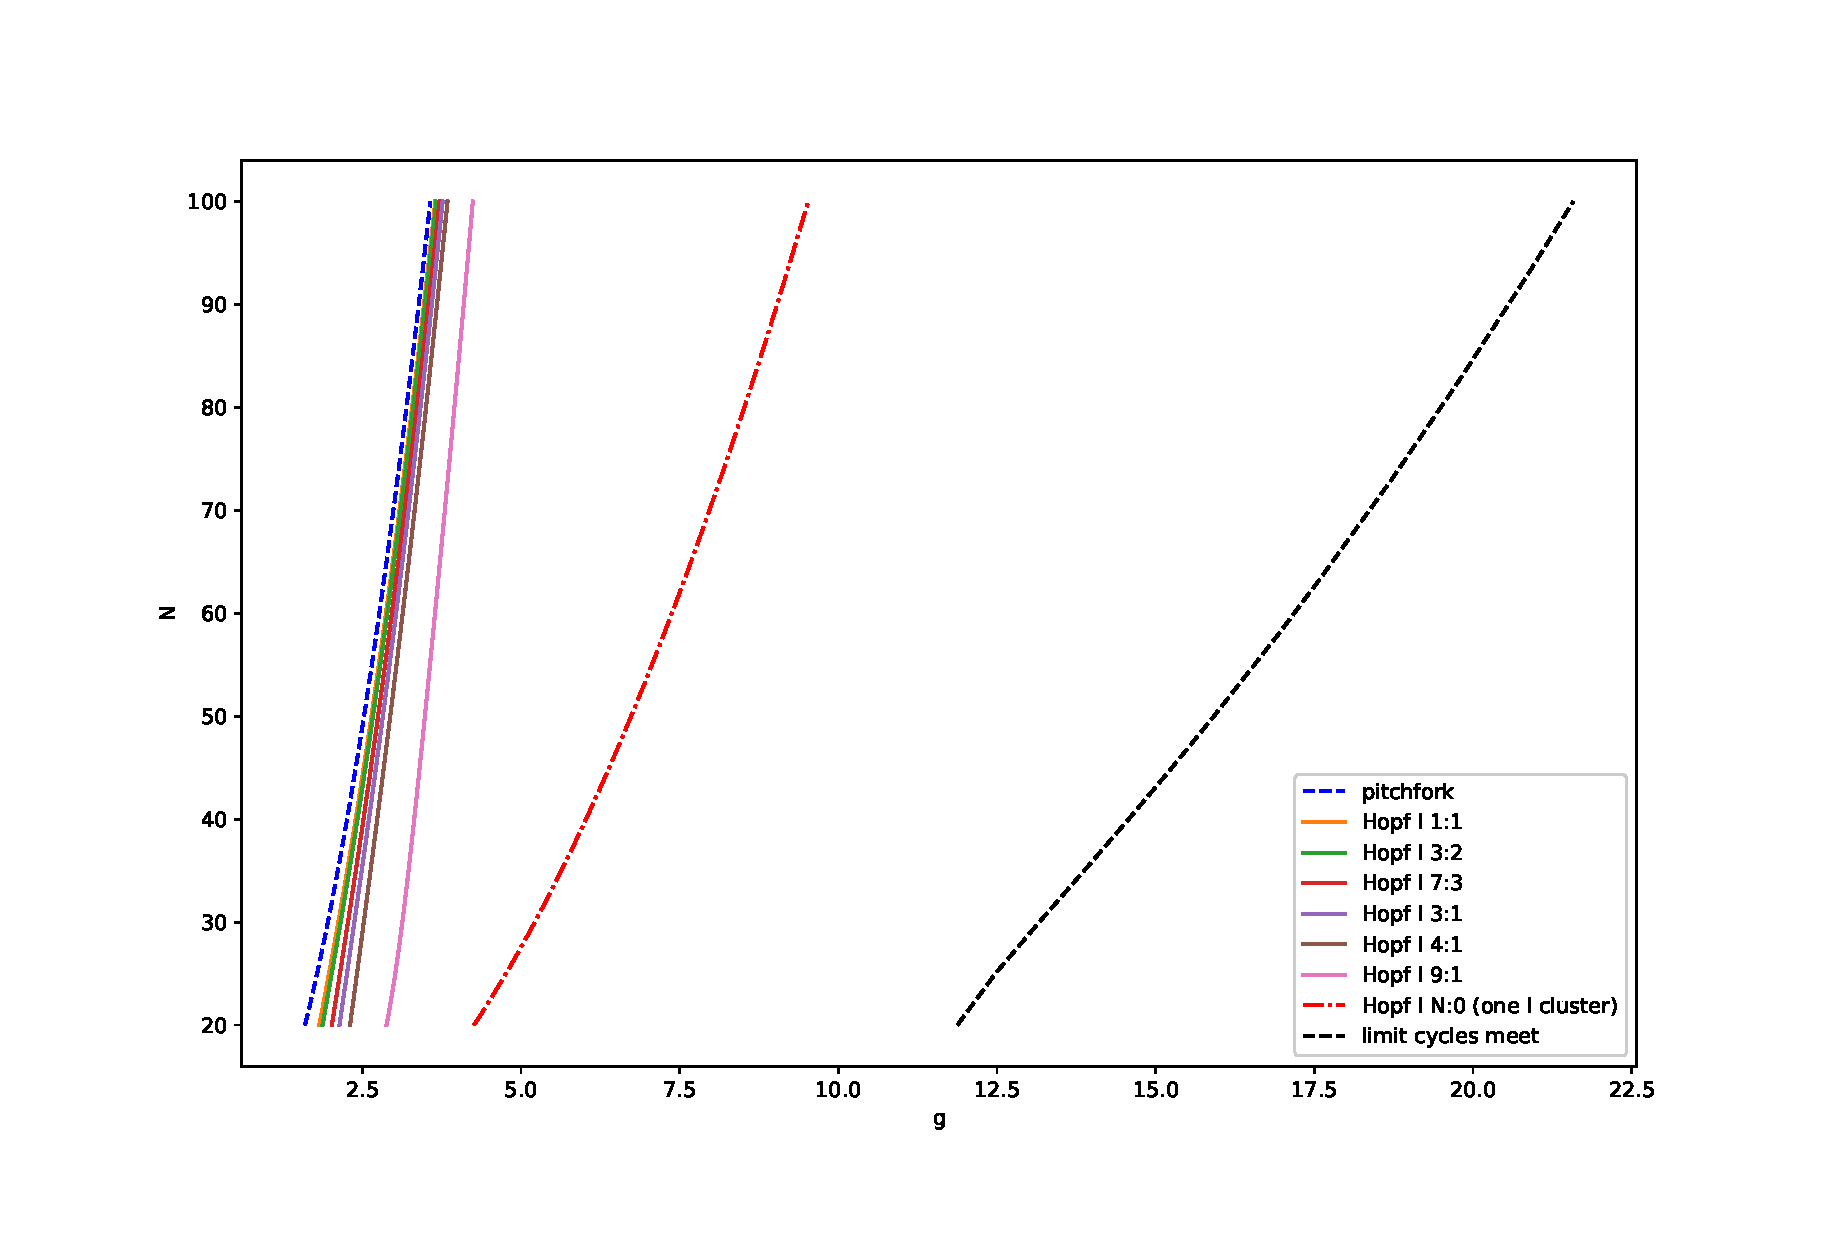
\includegraphics[width=15cm]{images/noclustersNvsg.eps}
    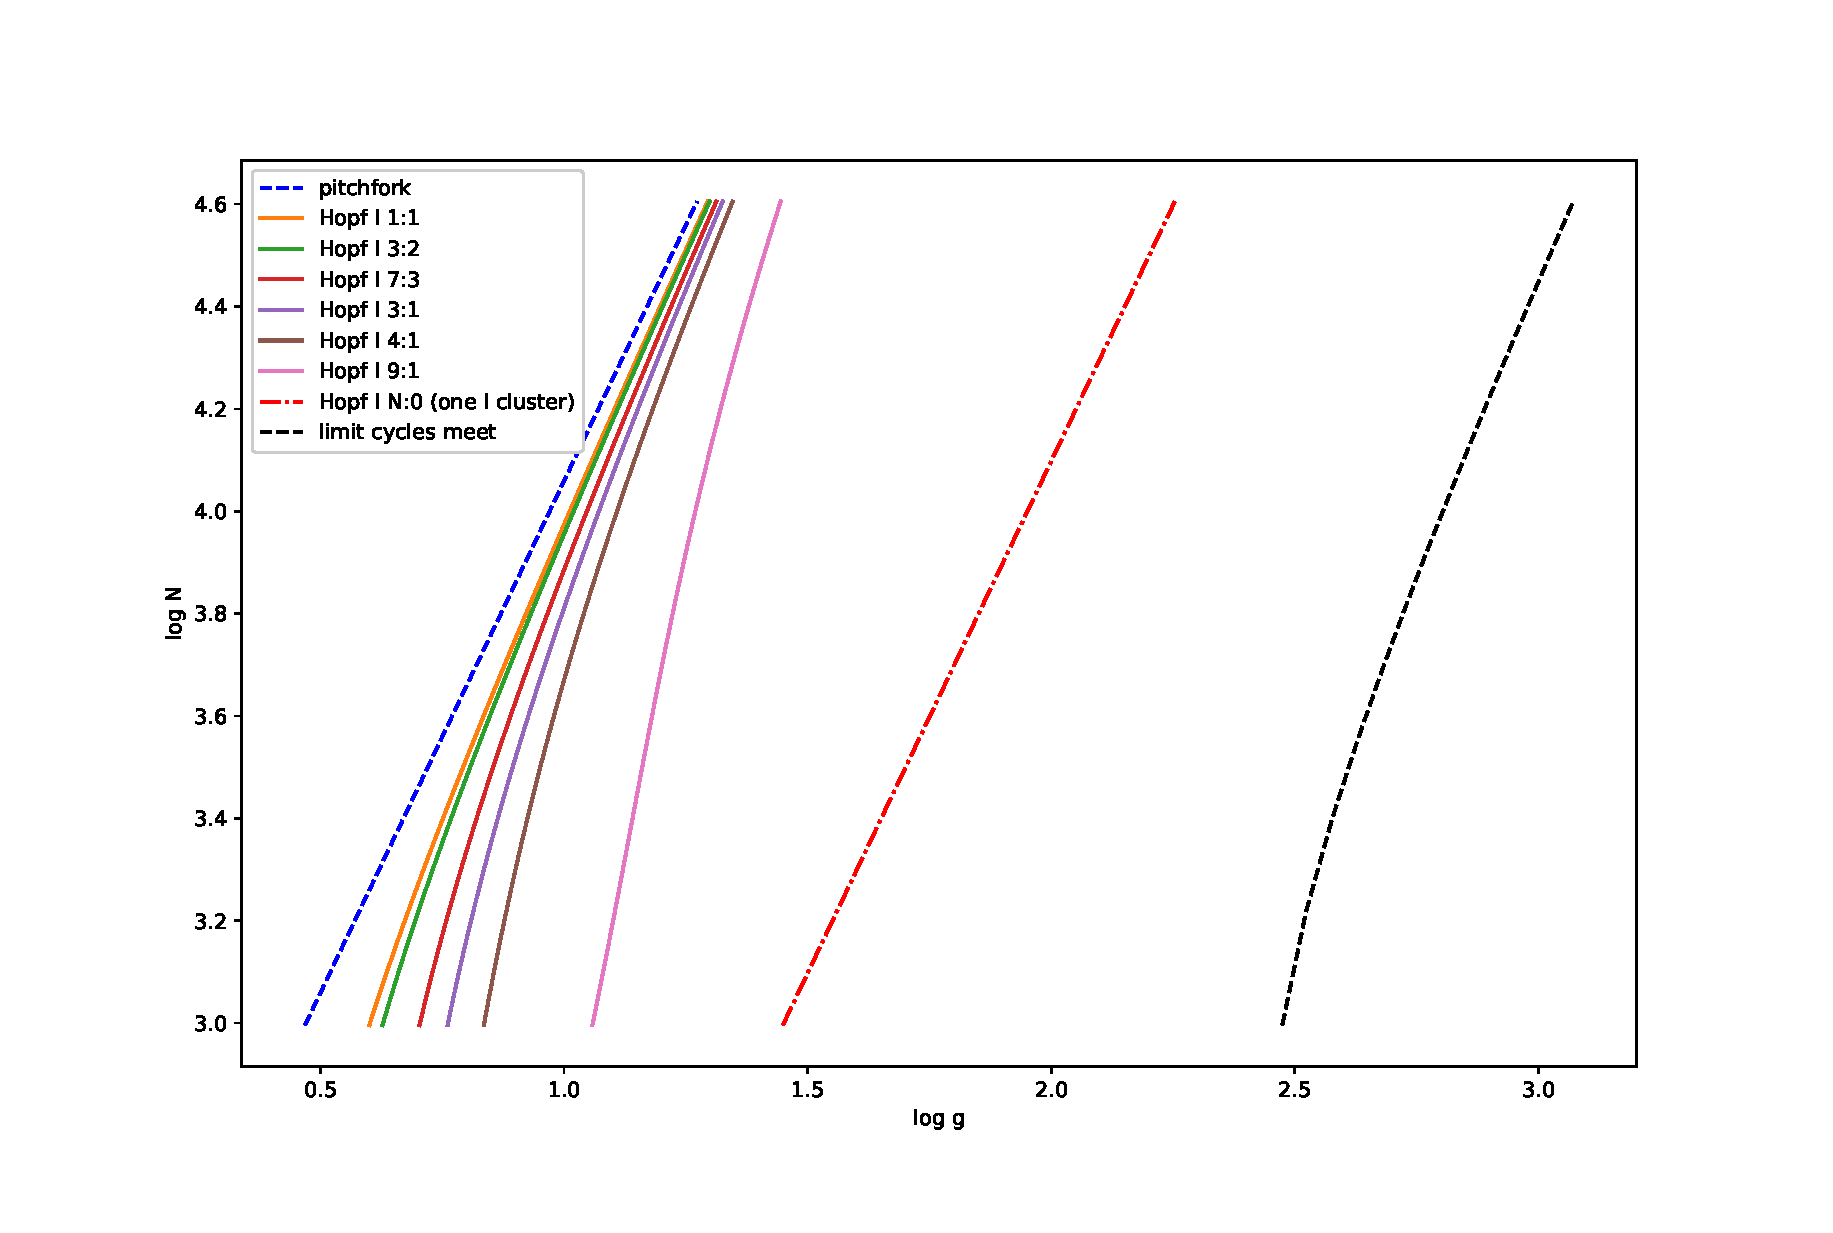
\includegraphics[width=15cm]{images/noclusterslogNvslogg.eps}
    \caption{Location in $g$ of pitchfork bifurcation, select Hopf bifurcations, and point where limit cycles meet for varying $N$. Lines are labeled from left to right.}
    \label{fig:periodvsg}
\end{figure}


Next plot is of stable limit cycle for case where all E-cells and I-cells are in sync, for large $g$. Plot is over one period (period is normalized to 1).

\begin{figure}[H]
    \centering
    \begin{tabular}{cc}
    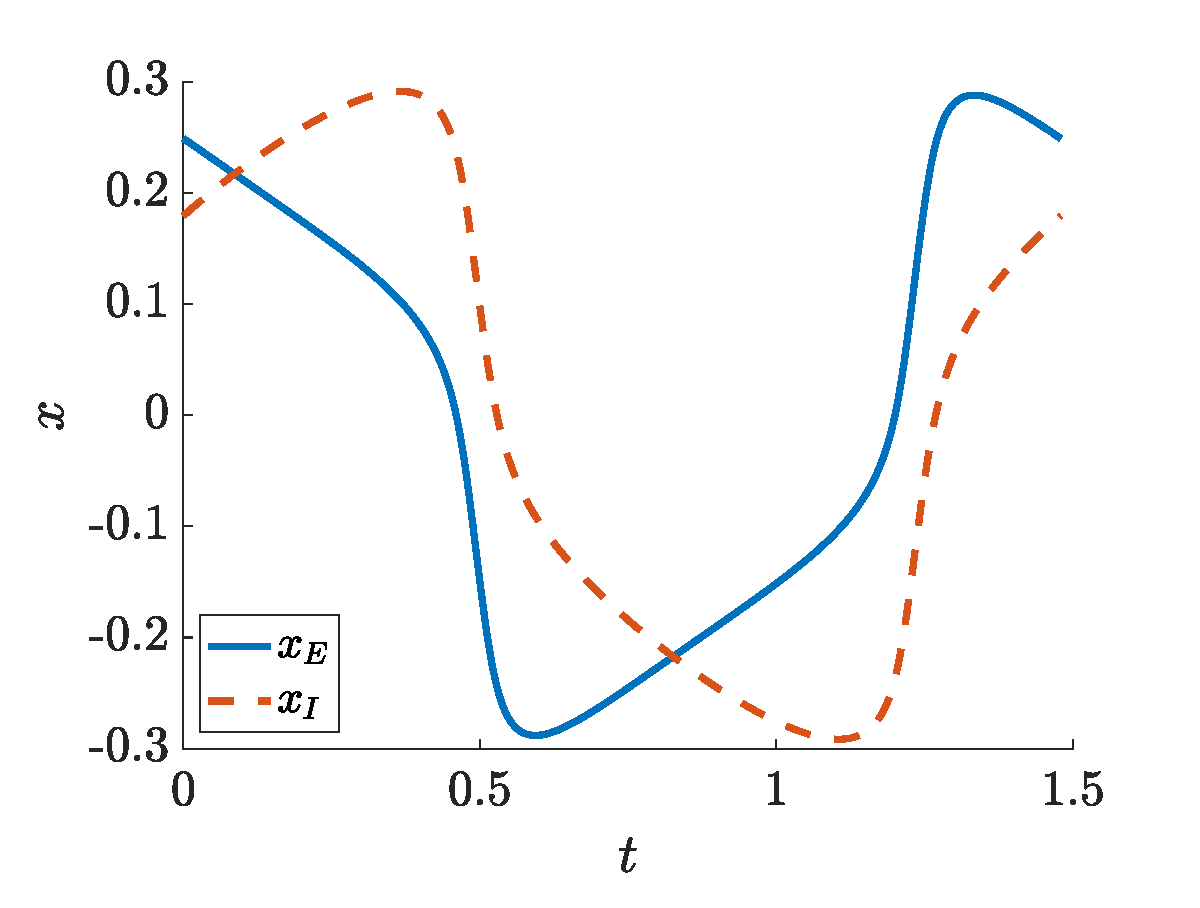
\includegraphics[width=8cm]{images/limitcycle1.eps}
    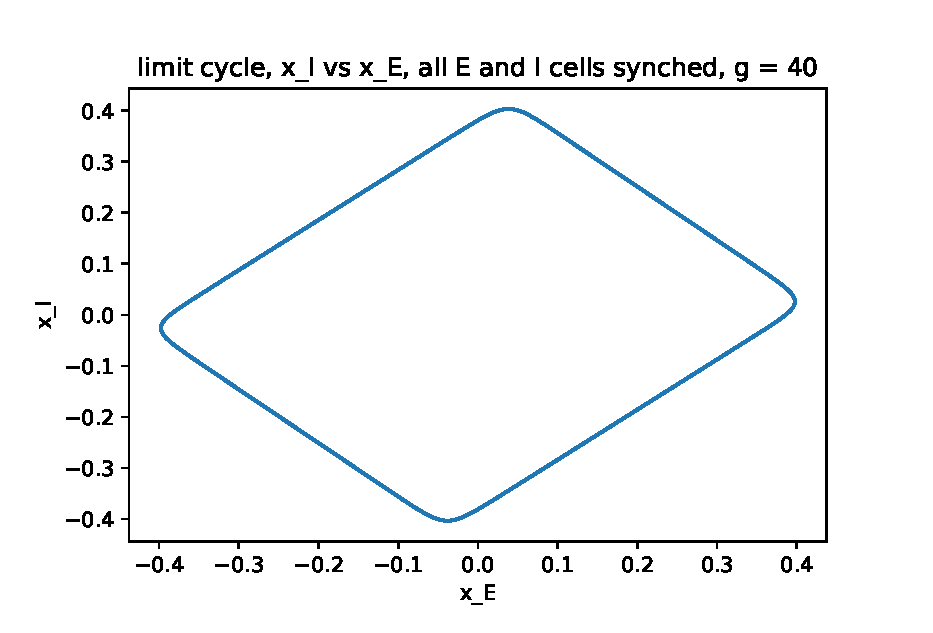
\includegraphics[width=8cm]{images/limitcycle2.eps}
    \end{tabular}
    \label{fig:limitcyclelargeg}
\end{figure}


\section{Excitatory clusters, weight parameters unchanged}

We now allow the excitatory cells to be grouped into $N_c$ clusters of size $p$, where $p = \lfloor N f/N_c \rfloor$. Cells will be connected within, but not between, clusters.
We still keep weights as in the previous section,  so that $\mu_{II} = -\alpha\mu_{IE}$ and $\mu_{EI} = -\alpha\mu_{EE}$.

Our matrix $H$ is now
\[
H = \frac{1}{\sqrt{N}}
\left[ 
\begin{blockarray}{ccccc}
\begin{block}{cccc|c}
\mu_{EE}\Kvec_{p} & 0 & \hdots & 0 & \BAmulticolumn{4}{c}{\multirow{4}{*}{$\mu_{EI}\Onevec_{n_E \times n_I}$}}\\
0 & \mu_{EE} \Kvec_{p} & \hdots & 0 &&&&\\
\vdots & \vdots & \ddots & 0 &&&&\\
0 & 0 & \hdots & \mu_{EE} \Kvec_{p} &&&&\\
\end{block} 
\cline{1-8}
\begin{block}{cccc|c}
&&&&\\
\BAmulticolumn{4}{c|}{\mu_{IE}\Onevec_{n_I \times n_E}} & \mu_{II} \Kvec_{n_I}\\
\end{blockarray}
\right]
\]

The symmetry group is now:
\[ 
\Gamma = \underbrace{S_{p} \oplus \cdots  \oplus S_{p}}_{N_c} \oplus \, S_{n_I}, \; p = fN/N_c \]


The eigenvalues of $\Hvec$ are:
\begin{itemize}
\item $\lambda_E = -\mu_{EE}$ with multiplicity $(p-1) \times N_c = n_E - N_c$.
\item $\lambda_I = -\mu_{II} = \alpha \mu_{EE}$ with multiplicity  $n_I - 1$
\item $\lambda_c = (p-1) \mu_{EE}$, with multiplicity $N_c - 1$.
\item Two remaining eigenvalues, given by the eigenvalues of:
 \begin{eqnarray}
\tilde{\Jvec} & = & \left[  \begin{matrix}
(p-1) \mu_{EE} & n_I \mu_{EI}\\[0.3em]
n_E  \mu_{IE}  & (n_I-1) \mu_{II}
\end{matrix} \right]   
\end{eqnarray}
\end{itemize}


The eigenvalues that are important for assessing the linearization of $-I + \frac{g}{\sqrt{N}} H$ are
\begin{align*}
    \lambda_c &= \frac{g}{\sqrt{N}} \left( \frac{f N}{N_c} - 1  \right)\mu_{EE} - 1 = \frac{g}{\sqrt{N}} \left( p - 1  \right) \mu_{EE} - 1  \\
    \lambda_I &= \frac{g\alpha}{\sqrt{N}} \mu_{EE} - 1
\end{align*}
When $\mu_{IE} = \mu_{EE}$, the matrix $\tilde{\Jvec}$ has eigenvalues
\[
\frac{\mu_{EE}}{2}\left( (p-1) - \alpha(N_i - 1) \pm \sqrt{ \left[ (p-1) +  \alpha(n_I - 1) \right]^2 - 4 \alpha n_I n_E} \right)
\]
Assuming the quantity under the radical sign is negative (\textbf{we can probably show this; it's true numerically}), $\tilde{\Jvec}$ has a complex conjugate pair of eigenvalues with real part
\[
\text{Re} \lambda = \frac{\mu_{EE}}{2}\left( (p-1) - \alpha(N_i - 1) \right)
\]
Substutiting $p = n_E/N_c$, factoring out $n_E$, and writing $n_E$ in terms of $N$ and $\alpha$, this becomes 
\[
\text{Re} \lambda = \frac{\mu_{EE}}{2}
\frac{\alpha N}{\alpha + 1}
\left( \frac{1}{N_c} - 1 + \frac{\alpha^2-1}{\alpha N} \right)
\]
For the standard value of $\alpha = 4$, $\text{Re} \lambda < 0$ whenever $N_c > 1$ and $N \geq 8$, which means that in this case, the Hopf bifurcation at the origin cannot happen since this eigenvalue cannot cross the imaginary axis.



Eigenvalue $\lambda_c$ crosses imaginary axis when 
\[
g = g_c = \frac{\sqrt{N}}{(p-1)\mu_{EE}}
\]
Eigenvalue $\lambda_I$ crosses imaginary axis when
\[
g = g_i = \frac{\sqrt{N}}{\alpha \mu_{EE}}
\]

We first consider the case where the excitatory clusters and inhibitory cells are divided into two population of equal size; the activity of each population has the same magnitude but opposite sign. We will refer to this as the symmetric branch. \textbf{Added definition of symmetric branch.} There are two cases to consider.
\begin{itemize}
    \item $N_c < \frac{fN}{\alpha+1}$ (small $N_c$)
    \item $N_c > \frac{fN}{\alpha+1}$ (large $N_c$)
\end{itemize}
\textbf{I changed "$<$" to "$=$" }
For now, ignore the degenerate case when $N_c = \frac{fN}{\alpha+1}$. When this happens, $\lambda_c = \lambda_I$.

\subsection{Symmetric branch, small $N_c$}
\begin{itemize}
    \item $\lambda_c > \lambda_I$, so $\lambda_c$ crosses imaginary axis first as $g$ increases. 
    \item Excitatory neurons branch off from 0 first when $g = g_c$, then inhibitory neurons branch off from 0 when $g = g_i$. (This is unlike the no clustering case, where inhibitory neurons branch off first).
    \item For symmetric branch, get equal numbers of clusters with opposite signs.
    \item Excitatory neurons branch off first when $g = g_c$. At this point, inhibitory neurons are still 0. For symmetric branch, will have equal numbers of clusters with opposite signs $\pm X_E$, so \cref{eq:reducedsystem} simplifies to the single equation
    \[
    -x_E + \frac{p-1}{\sqrt{N}} \mu_{EE} \tanh(g x_E) = 0
    \]
    Using the definition of $g_c$, this further simplifies to
    \begin{equation}\label{eq:Xesymm}
    \tanh(g x_E) = g_c x_E
    \end{equation}
    \item Write this as 
    \[
    f(x, g) = \tanh(g x) - g_c x
    \]
    and change variables by letting $y =  g x$, $h = g_c/g$ to get
    \[
    f(y, h) = \tanh y - h y = 0
    \]
    which is smooth in $y$ and $h$. $f(0, h) = 0$ for all $h$, and for $h > 0$, 
    \[
    \lim_{h\rightarrow\infty}f(y,h) = -\infty
    \]
    Since
    \[
    f_y(y, h) = \sech^2 y - h
    \]
    when $h > 1$, $f_y(y, h) < 0$ for all $y > 0$, which implies that $f(y, h) < 0$ for all $y > 0$, so $y = 0$ is the only solution to $f(y, h) = 0$. When $0 < h < 1$, $f_y(0, h) = 1 - h > 0$, so $f(y, h)$ is increasing at $y = 0$. By the smoothness of $f$ (and the IVT), $f(y_E, h) = 0$ for some $y_E > 0$. Since for fixed $h < 1$  and for $y>0$, $f(y,h)$ has a singe local maximum at $y = \cosh^{-1} \frac{1}{\sqrt{h}}$, $y_E$ is the unique, positive solution to $f(y, h) = 0$.  Undoing the change of variables, if $g > g_c$, $f(x, g) = 0$ has a unique positive solution $X_E$, which is what we want.
    
    \item We also note here that as $g \rightarrow \infty$, $\tanh(g x) \rightarrow 1$ for $x > 0$, thus we have 
    \[
    x_E \rightarrow \frac{1}{g_c} \text{ as }g \rightarrow \infty
    \]
    
    \item To leading order,
    \[
    x_E = \sqrt{ \frac{3(g-g_c)}{g^3} }
    \]
    for $g$ greater than, but close to $g_c$. This follows by Taylor expansion as in the single cluster case, replacing $g_0$ is replaced by $g_c$.
    
    \item Using the same argument, the inhibitory neurons branch off when $g = g_i$. If either all excitatory clusters are 0 or we have equal numbers of excitatory cluster with opposite activity, the excitatory terms do not contribute to the equations for the inhibitory neurons in \cref{eq:reducedsystem}. For the symmetric branch, there will be two populations of inhibitory neurons with opposite signs $\pm x_I$. By the same argument above, $x_I$ solves
    \[
    \tanh(g x_I) = g_i x_I
    \]
    which has a nonzero solution for $g > g_I$. 
    \item If both excitatory and inhibitory neurons are symmetric, the two populations behave independently, since the contribution from the other population in \cref{eq:reducedsystem} cancels.
\end{itemize}

Now that we know these symmetric solutions exist for $g > g_c$, we can analyse their stability. First look at the region $g_c < g < g_i$, where we have symmetric branch of excitatory neurons only.
\begin{itemize}
    \item Linearization about symmetric $x_E$ solution same as linearization about origin, except parameter $\mu_{EE}$ is replaced with
    \[
    \mu_{EE} \mapsto \sech^2( g x_E ) \mu_{EE}
    = (1 - g_c^2 x_E^2 )\mu_{EE} 
    \]
    \item Will denote eigenvalues of linearization about this solution by $\lambda^*$ with appopriate subscripts.
    \item Conjugate pair still has negative real part, $\lambda^*_e$ still negative, $\lambda^*_i$ unchanged, so only need to look at $\lambda^*_c$ which is given by
    \[
    \lambda^*_c(g) = \frac{g}{\sqrt{N}}(p-1)(1 - g_c^2 x_E(g)^2 )\mu_{EE} - 1= \frac{g}{g_c}(1 - g_c^2 x_E(g)^2) - 1
    \]
    \item When $g = g_c$, $x_E(g) = 0$, so $\lambda_c(g) = 0$
    \item As $g \rightarrow \infty$, $x_E(g) \rightarrow 1/g_c$ (see above), thus since $\lambda^*_c(g)$ is smooth,
    \[
    \lambda^*_c(g) \rightarrow -1 \text{ as } g \rightarrow \infty
    \]
    \item If $\lambda^*_c(g) > 0$ for any $g > g_c$, then by the IVT would need $\lambda^*_c(g) = 0$ for some $g > g_c$. We will show that cannot happen, i.e. $\lambda^*(g) = 0$ implies $g = g_c$.
    \item Assume $\lambda^*_c(g) = 0$ for some $g > g_c$. Then 
    \[
    \lambda^*_c(g) = \frac{g}{g_c}\sech^2(g x_E(g) ) - 1 = 0
    \]
    which we can rearrange and solve for $g x_E$ to get
    \[
    g x_E = \cosh^{-1} \sqrt{\frac{g}{g_c}}
    \]
    Since $x_E$ solves $\tanh g x_E = g_c x_E$, substitute the expression for $g x_E$ into this and simplify to get
    \[
    \frac{g}{g_c} \tanh\left( \cosh^{-1} \sqrt{\frac{g}{g_c}} \right) = \cosh^{-1} \sqrt{\frac{g}{g_c}}
    \]
    Letting $h = \sqrt{g/g_c}$ and simplifying (thanks, Mathematica!) gives us
    \[
    \cosh( h \sqrt{h^2 - 1} ) = h
    \]
    This only has a solution when $h = 1$. There are many ways to see this, e.g. for $f(h)$ defined by 
    \[
    f(h) = \cosh( h \sqrt{h^2 - 1} ) - h,
    \]
    $f(1) = 0$ and the only critical point of $f(h)$ on $(0, \infty)$ is a local minimum at $h = 1$, which corresponds to $g = g_c$.
    \item We have shown that $\lambda_c^*(g) < 0$ for $g > g_c$. This solution loses stability when $\lambda_i^*$ crosses the imaginary axis, which occurs when $g = g_i$.
    
\end{itemize}

\begin{figure}[H]
\centering
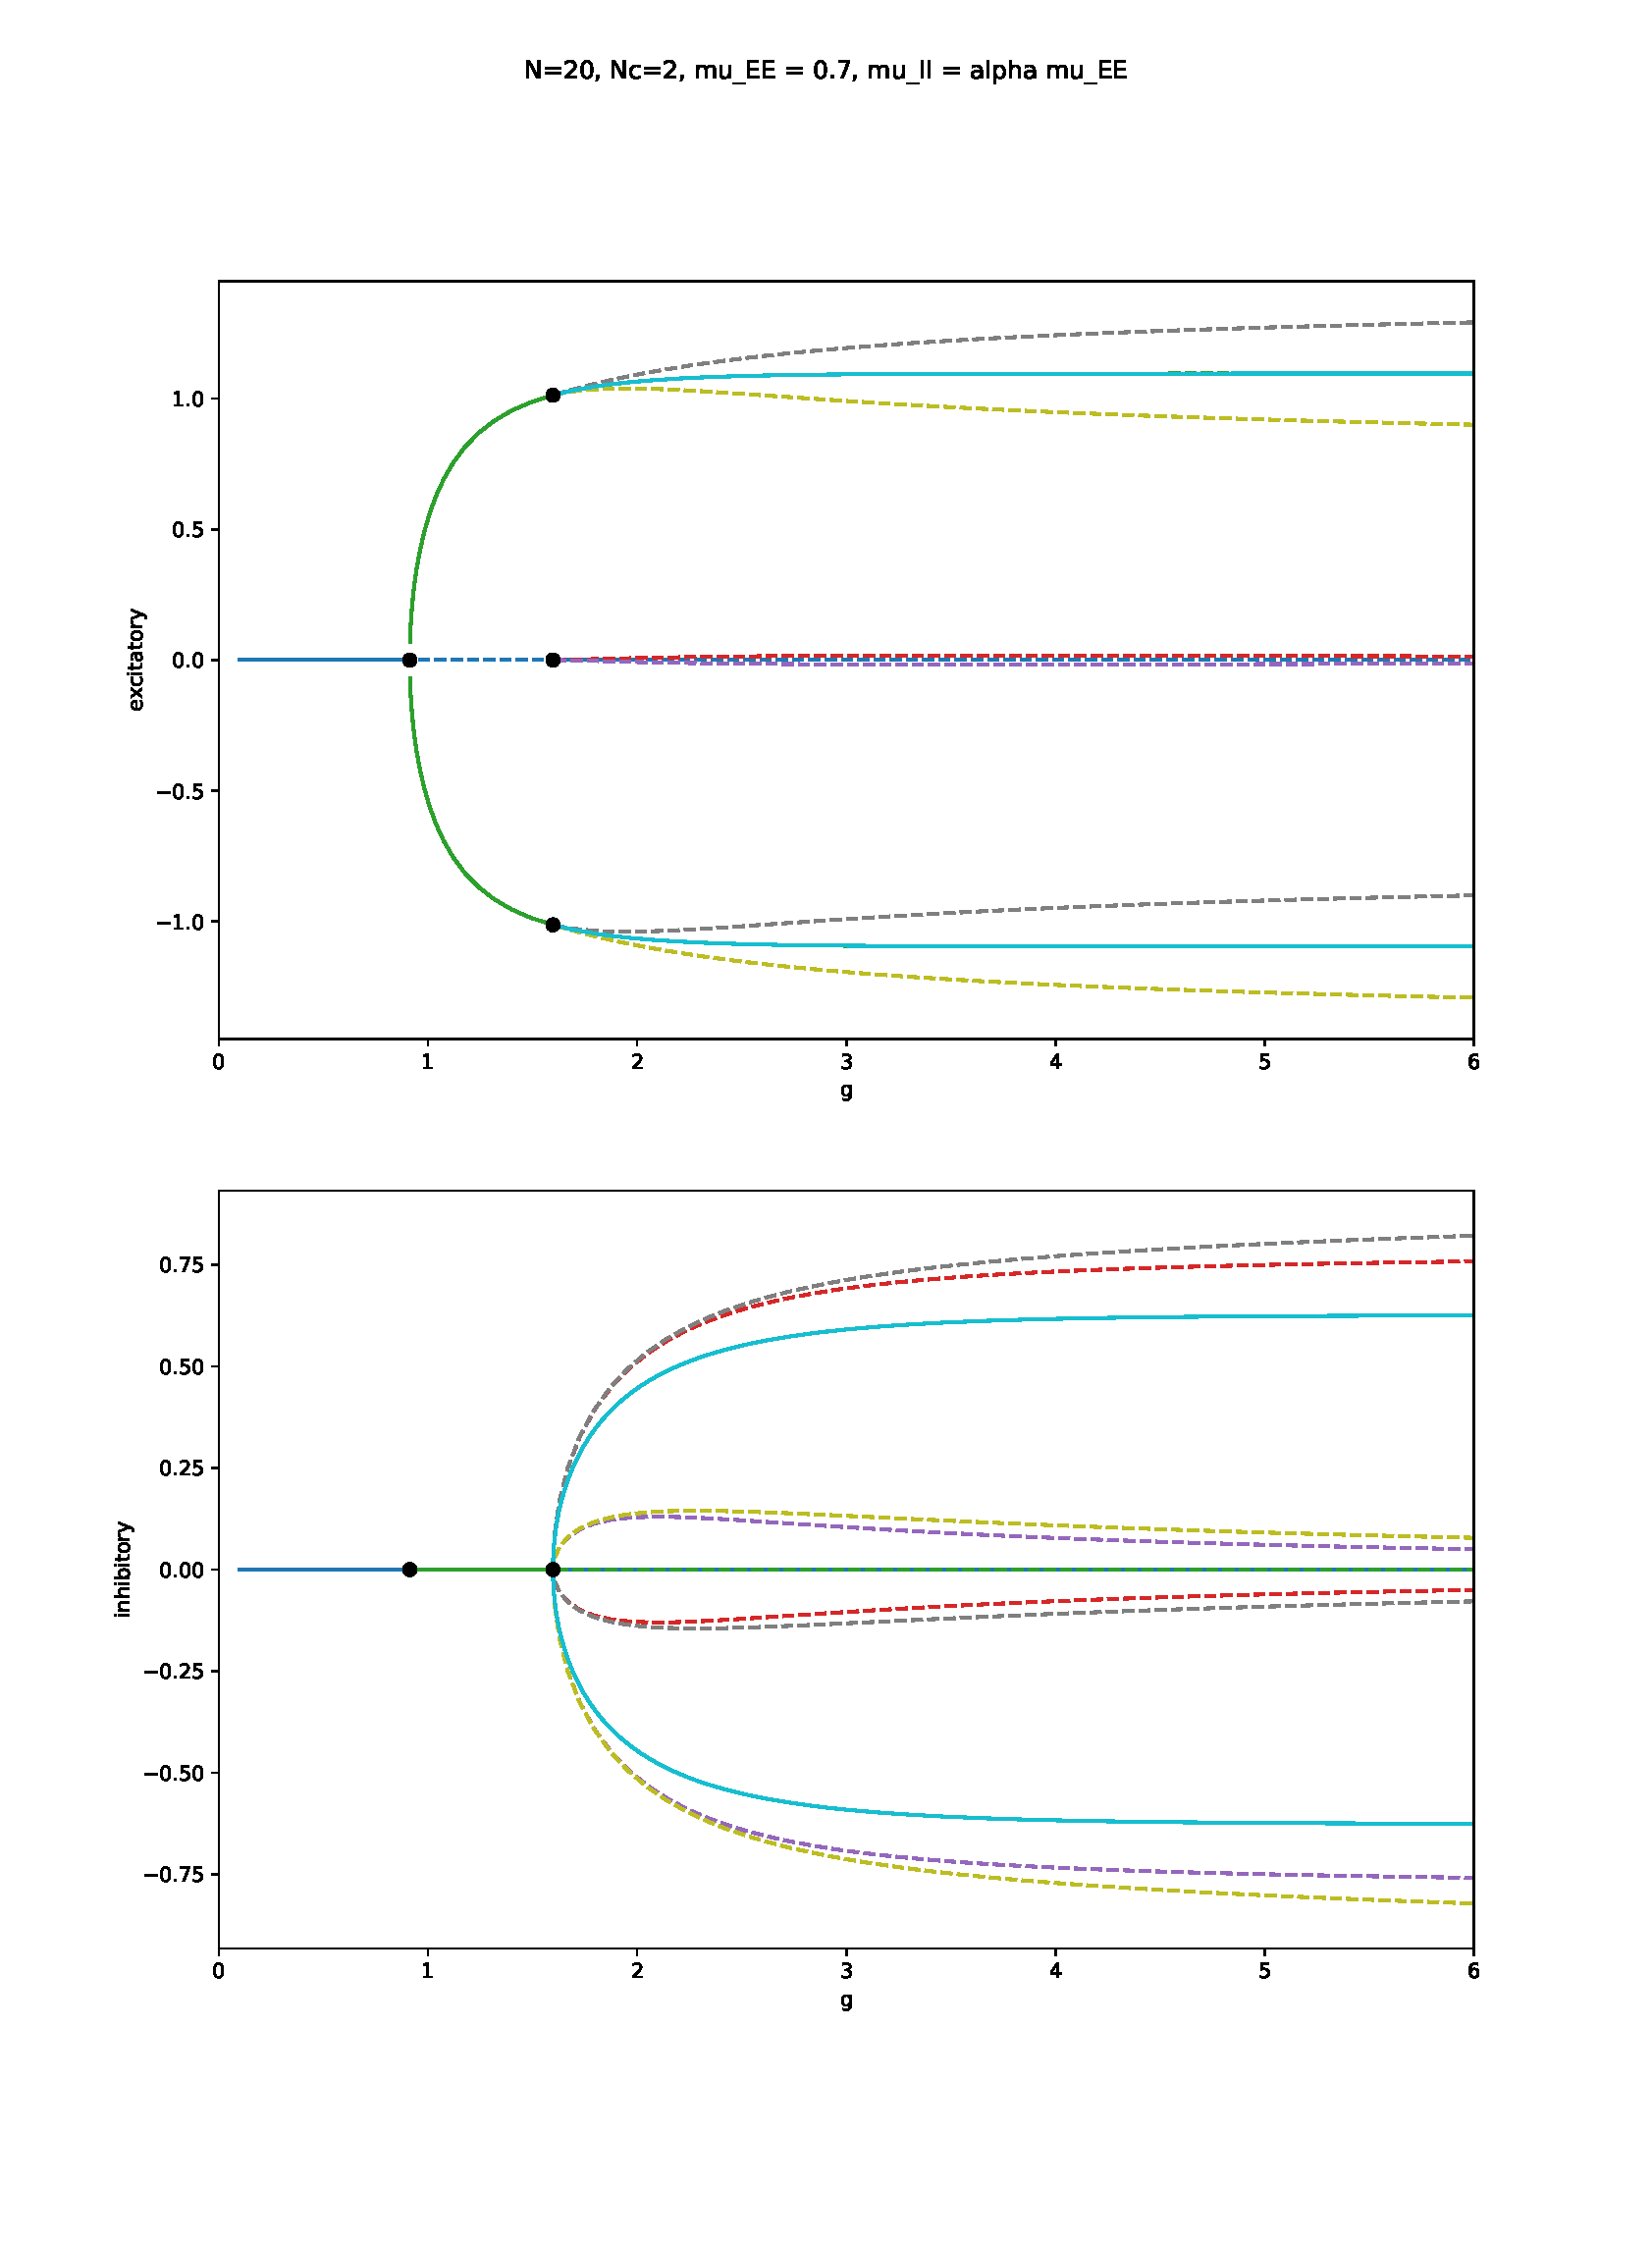
\includegraphics[width=14cm]{images/BD2_c20_E07.eps}
\end{figure}

Now we look at the region $g > g_i$, where we have symmetric branch of excitatory neurons at $x_E = x_E(g)$ and symmetric branch of inhibitory neurons at $x_I = x_I(g)$. Using the same argument as we did for $g_c < g < g_i$, this branch is stable for all $g > g_i$.

\subsection{Symmetric case, large $N_c$}
\begin{itemize}
    \item Symmetric branch: For $N_c > \frac{fN}{\alpha+1
    }$, $\lambda_i > \lambda_c$, so $\lambda_i$ crosses first as $g$ increases, leading to a symmetric branch of inbibitory neurons. $\lambda_c$ crosses next, leading to a symmetric branch of excitatory neurons. These symmetric branches are stable, by the same argument as the small $N_c$ case.
    
    \begin{figure}[H]
    \centering
    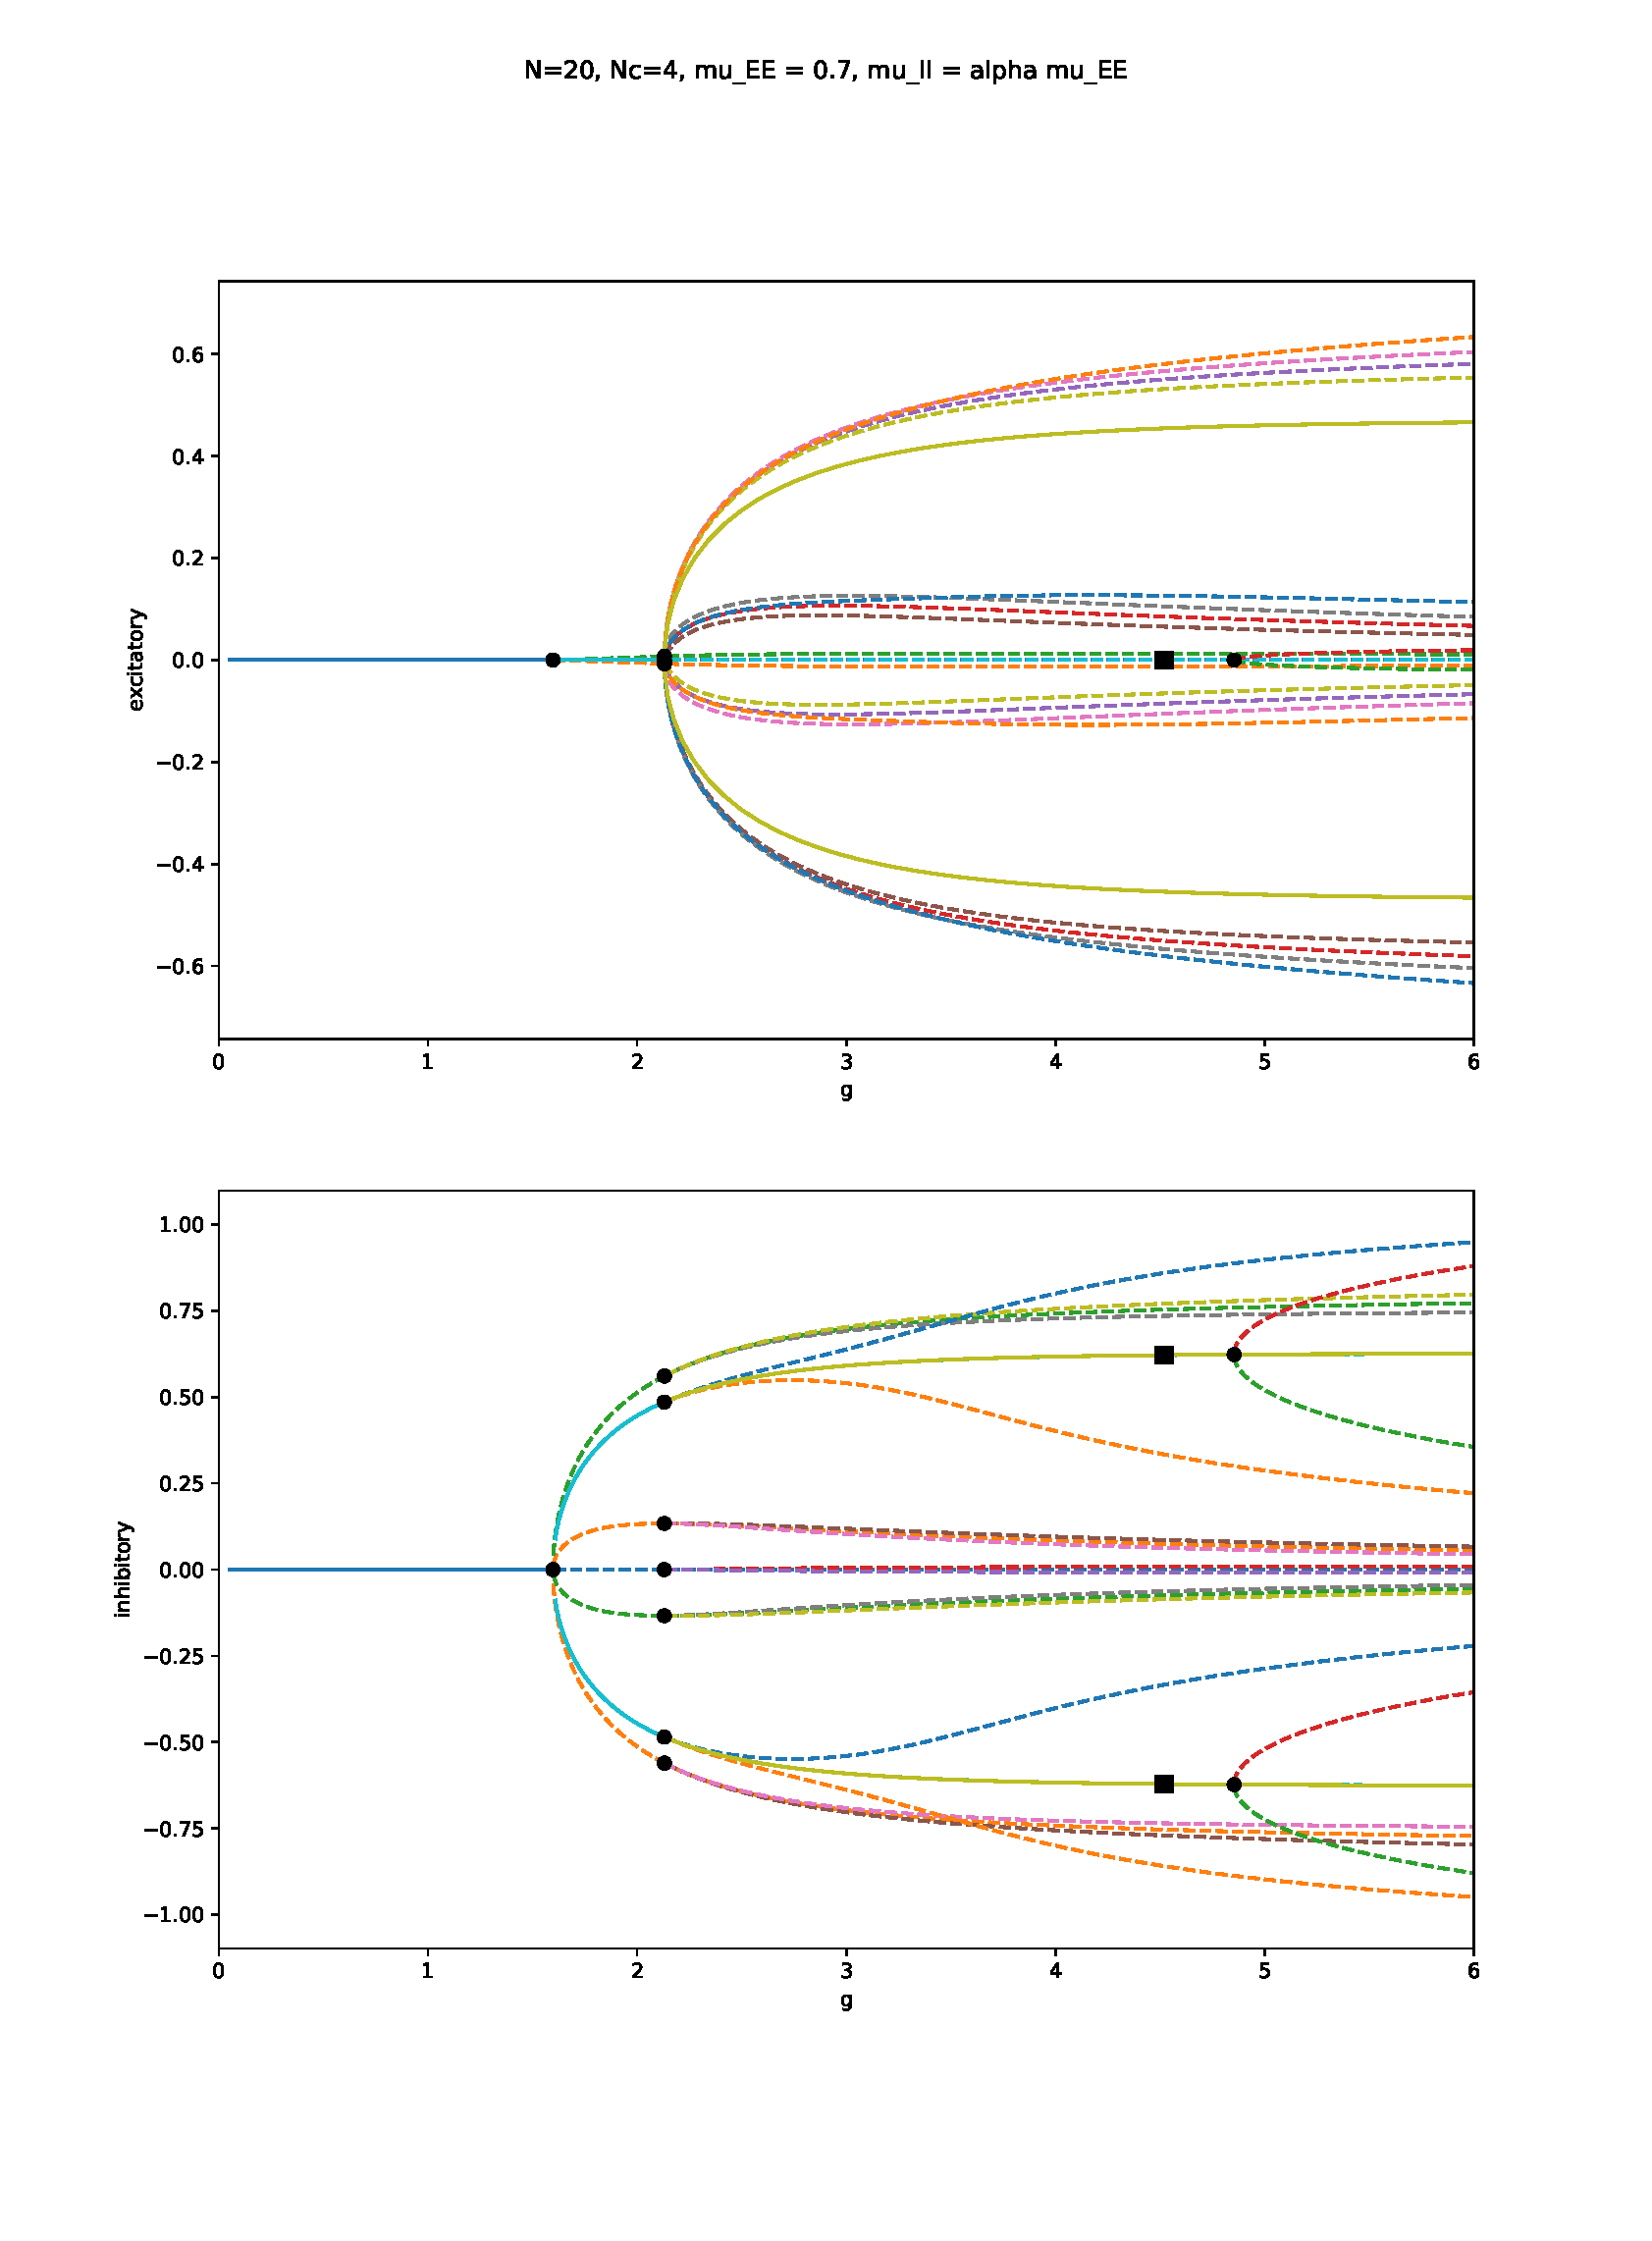
\includegraphics[width=14cm]{images/BD4_c20_E07.eps}
    \end{figure}
     
    \item In all cases, there is always a stable fixed point. Should be able to prove this, and that no Hopf bifurcations can happen on the symmetric branches. Numerical timestepping from random initial conditions confirms this.

\end{itemize}

\section{Excitatory clusters, parameter changed to restore balance}
Idea is to compensate for fewer excitatory connections by taking
\[
\mu_{EE} = -\frac{N_c}{\alpha} \mu_{EI}
\]
In this case, if we take $\mu_{EI} = \mu_{II}$, we have
\begin{align*}
g_i &= -\frac{\sqrt{N}}{\mu_{II}} \\
g_c &= -\frac{\alpha N}{(p-1)N_c \mu_{II}} 
= \frac{\alpha}{(p-1)N_c} g_i = 
\frac{N_E}{N_I( N_E - N_c)} g_i < g_i
\end{align*}
The excitatory clusters always branch off first since $g_c < g_i$. As above, there is always a stable, symmetric solution. This follows from the exact same argument.

\begin{figure}[H]
\centering
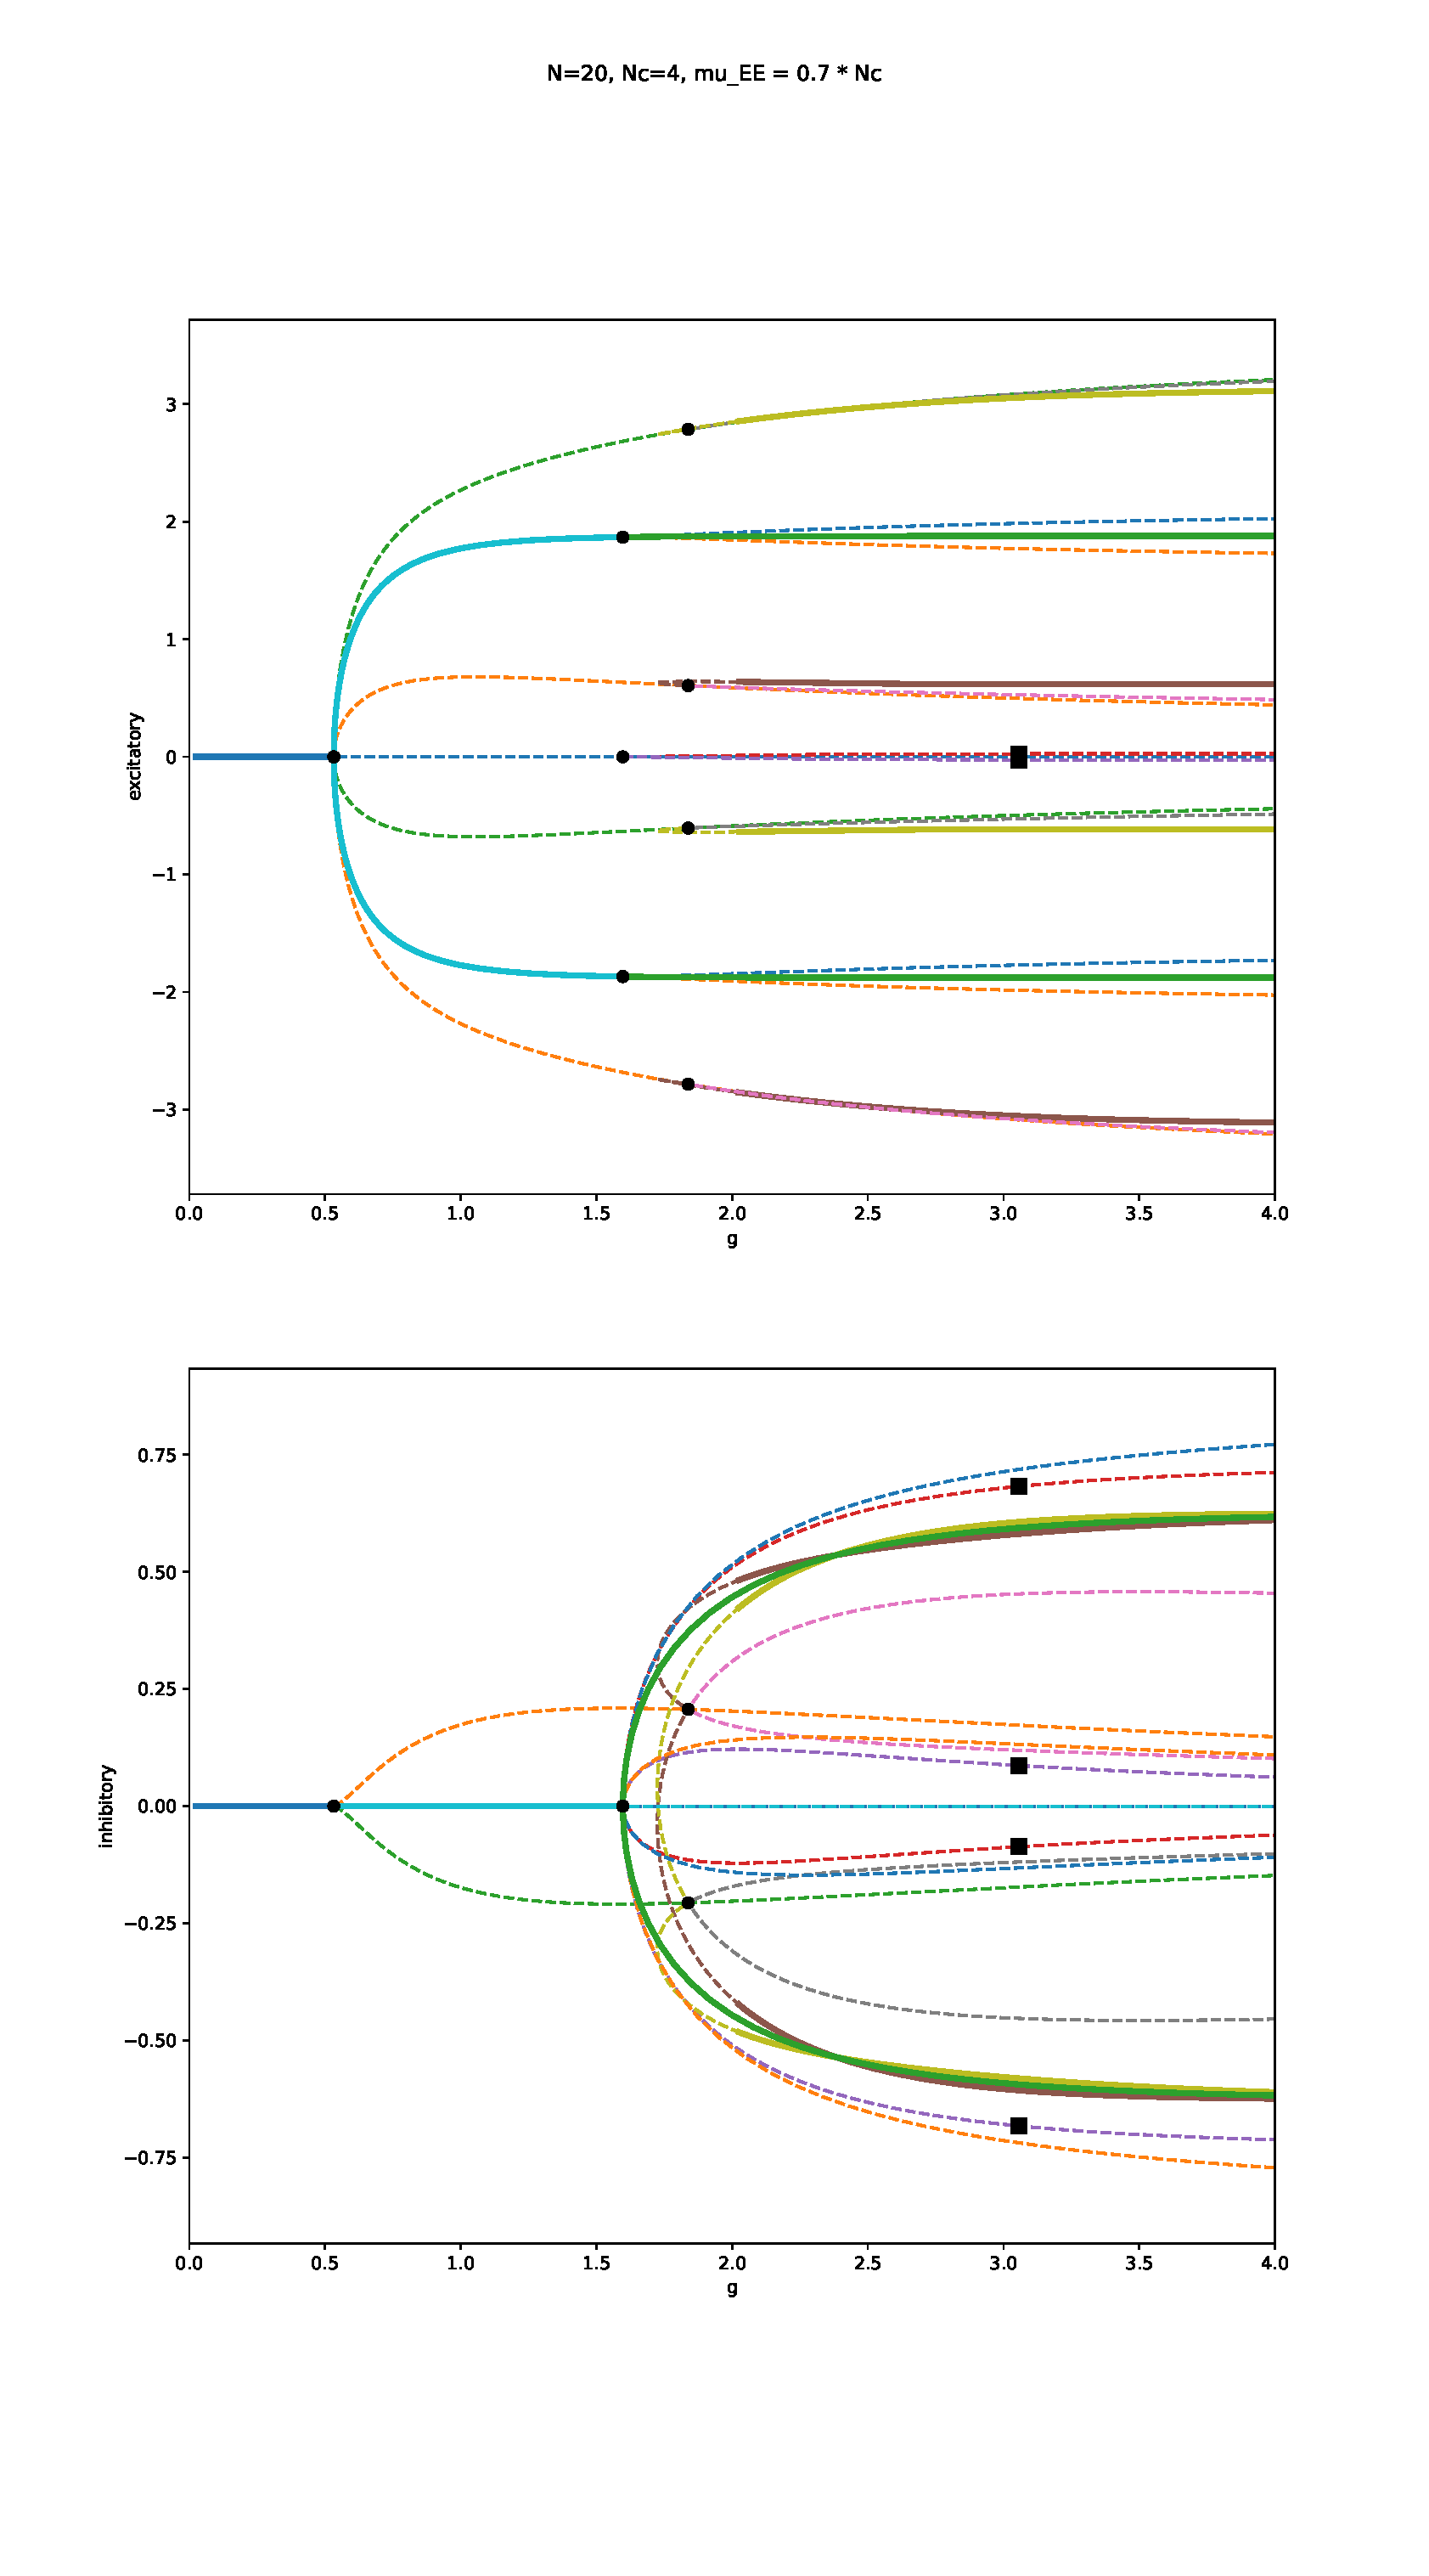
\includegraphics[width=10cm]{images/BD4a_c20.eps}
\end{figure}

\begin{itemize}
    \item From one example $N = 20$, 4 clusters: there is always a stable fixed point at a symmetric solution.
    
    \item For larger $g$, the symmetric fixed point coexists with asymmetric fixed points. This can be verified by timestepping from random initial conditions. Stable asymmetric fixed point is on a different branch from stable symmetric fixed point. There is a region of $g$ after $g$ passes $g_i$ for which only stable fixed point is the symmetric one.
    
    \item Same behavior occurs for higher $N$ and larger $N_c$, the main difference being that there are more stable, asymmetric fixed points for large $g$.
\end{itemize}

What happens for large $g$
\begin{itemize}
    \item The $\tanh(g x_j)$ are 0 if $x_j = 0$, otherwise are 1 if $x_j > 0$ and -1 if $x_j < 0$.
    \item This means that the equilbrium equation for each $x_j$ involves only the variable $x_j$, so for any given symmetry and set of signs, we can solve for the limiting equilibrium solution as $g$ gets large.
    \item Example: For the asymmetric stable equilibrium solutions above, the excitatory clusters are 3+/1-, and the inhibitory cells are also 3+/1-. Using this, we can solve for the limiting $x_j$, which agrees with the numerics.
    \begin{align*}
        x_{E1} &= \frac{1}{\sqrt{N}}\left( (p-1)\mu_{EE} + (3-1) \mu_{EI} \right) \\
        x_{E2} &= \frac{1}{\sqrt{N}}\left( -(p-1)\mu_{EE} + (3-1) \mu_{EI} \right) \\
        x_{I1} &= \frac{1}{\sqrt{N}}\left( (3-1)p\mu_{IE} + (2-1) \mu_{II} \right) \\
        x_{I2} &= \frac{1}{\sqrt{N}}\left( (3-1)p\mu_{IE} + 3 \mu_{II} \right) 
    \end{align*}
    None of these are 0.
    
    \item For another equilibrium solution: excitatory 4+, inhibitory 1+/3-, but solving these
        \begin{align*}
        x_{E} &= \frac{1}{\sqrt{N}}\left( (p-1)\mu_{EE} + (1-3) \mu_{EI} \right) \\
        x_{I1} &= \frac{1}{\sqrt{N}}\left( 4 p\mu_{IE} + (-3) \mu_{II} \right) \\
        x_{I2} &= \frac{1}{\sqrt{N}}\left( 4 p\mu_{IE} + (1-2) \mu_{II} \right) 
    \end{align*}
    does not give the solution we see. Likely what is happening here is that $X_{I1}$ has a nonzero limit, but the other two have limit of 0.
    
\end{itemize}

Which limiting solutions are stable?
\begin{itemize}
    \item For the stability analysis as $g \rightarrow \infty$, if the limiting value of any of the $x_j$ is nonzero, the corresponding $g \sech^2 g x_j$ term in the linearization goes to 0. In particular, if \emph{all} of the $x_j$ have nonzero limiting value, the Jacobian matrix has a limiting value of $-I$, thus all the eigenvalues have a limiting value of $-1$, which means that all of these solutions are stable. 
    
    \item The only way to have an unstable solution in the limit as $g \rightarrow \infty$ is to have at $x_j \rightarrow 0$ for at least one of the $x_j$.
    
    \item Hypothesis: If $x_j \rightarrow 0$ for at least one of the $x_j$, the corresponding equlibrium is unstable.
\end{itemize}

\subsection{A characterization of all large $g$ solutions}
Idea: use a matrix to determine valid solutions for large $g$.

Let $\mathbf{I}_n$ denote the $n\times n$ identity matrix, $\mathbf{1}_{m \times n}$ the $m\times n$ matrix of ones, and $\mathbf{K}_n$ the $n\times n$ matrix with all ones off the diagonal; i.e. $\mathbf{K}_n = \mathbf{1}_{n \times 1} \left( \mathbf{1}_{n \times 1}\right)^T - \mathbf{I}_n$. 
\begin{itemize}
\item Since we only have to solve the reduced system (one variable per excitatory cluster), define the $(N_c + N_I) \times (N_c + N_I)$ block matrix \textbf{Used xtra lines in matrix to give space: arraystretch might be better?}
\[
H_1 = \frac{1}{\sqrt{N}}
\left[ \begin{array}{c|c}
\\
(p-1)\mu_{EE} \mathbf{I}_{N_c} & \mu_{EI}\mathbf{1}_{N_c \times N_I}\\
\\
\hline
\\
p \mu_{IE} \mathbf{1}_{N_I \times N_C} & \mu_{II} \mathbf{K}_{N_I} \\
\\
\end{array}
\right]
\]

This is the original matrix $H$ (divided by $\sqrt{N}$) if you treat all excitatory cells in a single cluster as one cell.
\item For each potential large-$g$ solution, define the ``sign vector'' $\mathbf{v}$ by
\[
\mathbf{v} = (\text{sign}(x_{E1}), \dots, \text{sign} (x_{EN_c}), \text{sign} (x_{I1}), \dots, \text{sign} (x_{IN_I})
\]
where the sign is $1, -1$ or 0.
\item If a large-$g$ solution exists with that sign vector, then $H_1 \mathbf{v}$ will have the same signs as the sign vector $\mathbf{v}$ and the solution will be $H_1 \mathbf{v}$. For now, this is a necessary (but not sufficient) condition for the large-$g$ solution to exist. Hopefully it is also sufficient.
\item If all we want to know is whether such a solution can exist, we can use the relationships between the coefficients to simplify the matrix. Specifically, we assume that 
\[\begin{pmatrix}
\mu_{EE} & \mu_{EI}\\
\mu_{IE} & \mu_{II}
\end{pmatrix} \rightarrow 
\begin{pmatrix}
N_c \mu & -\alpha \mu\\
\mu & -\alpha \mu
\end{pmatrix}
 \]
 where we have expressed each coefficient in terms of $\mu = \mu_{IE}$, the $E\rightarrow I$ connection weight. Then $H_1$ simplifies 
to
\[
H_2 =
\left( \begin{array}{c|c}
(p-1)N_C\mathbf{I}_{N_c} & -\alpha \mathbf{1}_{N_c \times N_I}\\
\hline
p \mathbf{1}_{N_I \times N_C} & -\alpha \mathbf{K}_{N_I} 
\end{array}
\right)
\]
up to a constant.
%\[
%H_2 = 
%\begin{pmatrix}
%\text{diag}( (p-1)N_c) & -\alpha \\
%p & \text{offdiag}(-\alpha )
%\end{pmatrix}
%\]

Then a necessary condition for the large-$g$ solution to exist is that $H_2 \mathbf{v}$ and $\mathbf{v}$ have same signs.

\item Let $n_I^+$, $n_I^-$, and $n_I^0$ be the number of inhibitory cells which are positive, negative, and 0 in the large-$g$ limit. Let $b(I)$ be the ``balance'' of these, i.e.
\[
b(I) = n_I^+ - n_I^-
\]
Let $n_E^+$, $n_E^-$, and $n_E^0$ be the same thing for the excitatory clusters, and define the ``balance'' $b(E)$ the same way.
 
\end{itemize}

\subsubsection{Nonzero solutions}
\begin{itemize}
\item For now, assume there are excitatory clusters with both positive and negative $X_E$ and inhibitory neurons with both positive and negative $X_I$. (For homogeneous populations of one or the other, should be easier.) Also assume none of them are 0.  That is, we assume
 $n_E^+, n_E^-, n_I^+, n_I^- > 0$ and $n_E^0, = n_I^0 = 0$. Then the simplified equation 
\[ \text{sign}(H_2 \textbf{v}) = \text{sign}(\textbf{v}) \]
reduces to the conditions
\begin{align*}
&(p-1) N_c - \alpha b(I) > 0 && \text{positive excitatory} \\
-&(p-1) N_c - \alpha b(I) < 0 && \text{negative excitatory} \\
&p\:b(E) - \alpha (b(I)-1) > 0 && \text{positive inhibitory} \\
&p\:b(E) - \alpha (b(I)+1) < 0 && \text{negative inhibitory} 
\end{align*}

\item The first pair of inequalities are satisfied if and only if
\[
|b(I)| < \frac{(p-1) N_c}{\alpha}
\]
which constrains how the inhibitory cells can be split up. We can simplify the RHS using
\begin{align*}
\frac{(p-1) N_c}{\alpha}
&= (p-1) N_c \frac{N_I}{N_E}
= p N_c \frac{N_I}{N_E} - N_c \frac{N_I}{N_E} = N_I - N_c \frac{N_I}{N_E}
= N_I\left( 1 - \frac{N_c}{N_E} \right) \\
&= N_I\left( 1 - \frac{1}{p} \right)
\end{align*}
so this becomes
\[
|b(I)| < N_I\left( 1 - \frac{1}{p} \right)
\]
Since $p > 1$, this means that $|b(I)| <  N_I$, i.e. we cannot have $|b(I)| = N_I$, so there cannot be a homogeneous, nonzero population of inhibitory cells.

\item The second pair of inequalities are satisfied if and only if
\[
\frac{\alpha}{p}(b(I)-1) < b(E) < \frac{\alpha}{p}(b(I)+1)
\]
Multiply this by $N_I/N_c$ and simplify
\begin{align*}
&\frac{N_I \alpha}{N_c p}(b(I)-1) < \frac{N_I}{N_c} b(E) < \frac{N_I \alpha}{N_c p}(b(I)+1) \\
&\frac{N_I \alpha}{N_E}(b(I)-1) < \frac{N_I}{N_c} b(E) < \frac{N_I \alpha}{N_E}(b(I)+1) \\
&b(I)-1 < \frac{N_I}{N_c} b(E) < b(I)+1
\end{align*}

\item If $\frac{N_I}{N_c} b(E)$ is an integer, then we can say more, since
\[
\frac{N_I}{N_c} b(E) = b(I)
\]
which means that
\[
\frac{b(E)}{N_c} = \frac{b(I)}{N_I}
\]
Since $N_c = N_E^+ + N_E^-$ and $N_I = N_I^+ + N_I^-$, we can do some algebra to get
\[
\frac{N_E^+}{N_I^+} = \frac{N_E^-}{N_I^-} =
\frac{N_c}{N_I}
\]
from which it follows that
\[
\frac{N_E^+}{N_E^-} = \frac{N_I^+}{N_I^-},
\]
i.e. the ratio of positive to negative is the same for inhibitory cells and excitatory clusters!

\item If $\frac{N_I}{N_c} b(E)$ is not an integer, the inequalities still hold, but we no longer have the same ratio.

\end{itemize}

\subsubsection{Solutions with some zeros}

\textbf{Conjecture:} These may never happen unless the cell is 0 for all $g$.

\begin{itemize}
\item If $N_E^0 \neq 0$, i.e. there is at least one excitatory cluster which is 0 in the large $g$ limit, then we have the additional equation $0(p-1)N_c - \alpha b(I) = 0$, from which it follows that $b(I) = 0$. The inequality for $b(E)$ then becomes
\[
-\frac{\alpha}{p} < b(E) < \frac{\alpha}{p}
\]
Since $\alpha = N_E/N_I = N_c p/N_I$, this becomes
\[
-\frac{N_c}{N_I} < b(E) < \frac{N_c}{N_I}
\]
This means that if $N_c \leq N_I$, we must have $b(E) = 0$ as well. There are more possibilities if $N_c > N_I$.

\item If $N_I^0 \neq 0$, i.e. there is at least one inhibitory cluster which is 0 in the large $g$ limit, then we have the additional equation 
\[
p b(E) - \alpha b(I) = 0
\]
which implies
\[
b(E) = \frac{\alpha}{p} b(I) = \frac{N_c}{N_i} b(I)
\]

\end{itemize}

\subsubsection{Solutions with $\tanh(gx) \rightarrow r$, $0 < \vert r \vert < 1$}

A final possibility is that there are degrees of freedom for which $x_k \rightarrow 0$, but in such as way that $g x_k \rightarrow c$ for some real constant $c$. Then $\tanh(gx) \rightarrow r$, $0 < \vert r \vert < 1$. Deriving such solutions becomes considerably more complicated, as we have not only a linear matrix equation, but nonlinear consistency conditions relating $x_k$ and $\tanh(g x_k)$ \textbf{Actually LHS is zero for large g: still more complicated than $\pm$ 1}

Instead of proceeding along these lines, we will show that all such solutions are unstable.

\subsection{Plots}

Plots below illustrate these large $g$ results. Stable solutions for large $g$ are those predicted. (Exception: there is symmetric solution for $N=37$ for which one I-cell is 0. This one is also eventually stable. Should not be hard to show this, since symmetric). Can do this for more complicated arrangements, but the plots get cluttered.

\begin{figure}[H]
\centering
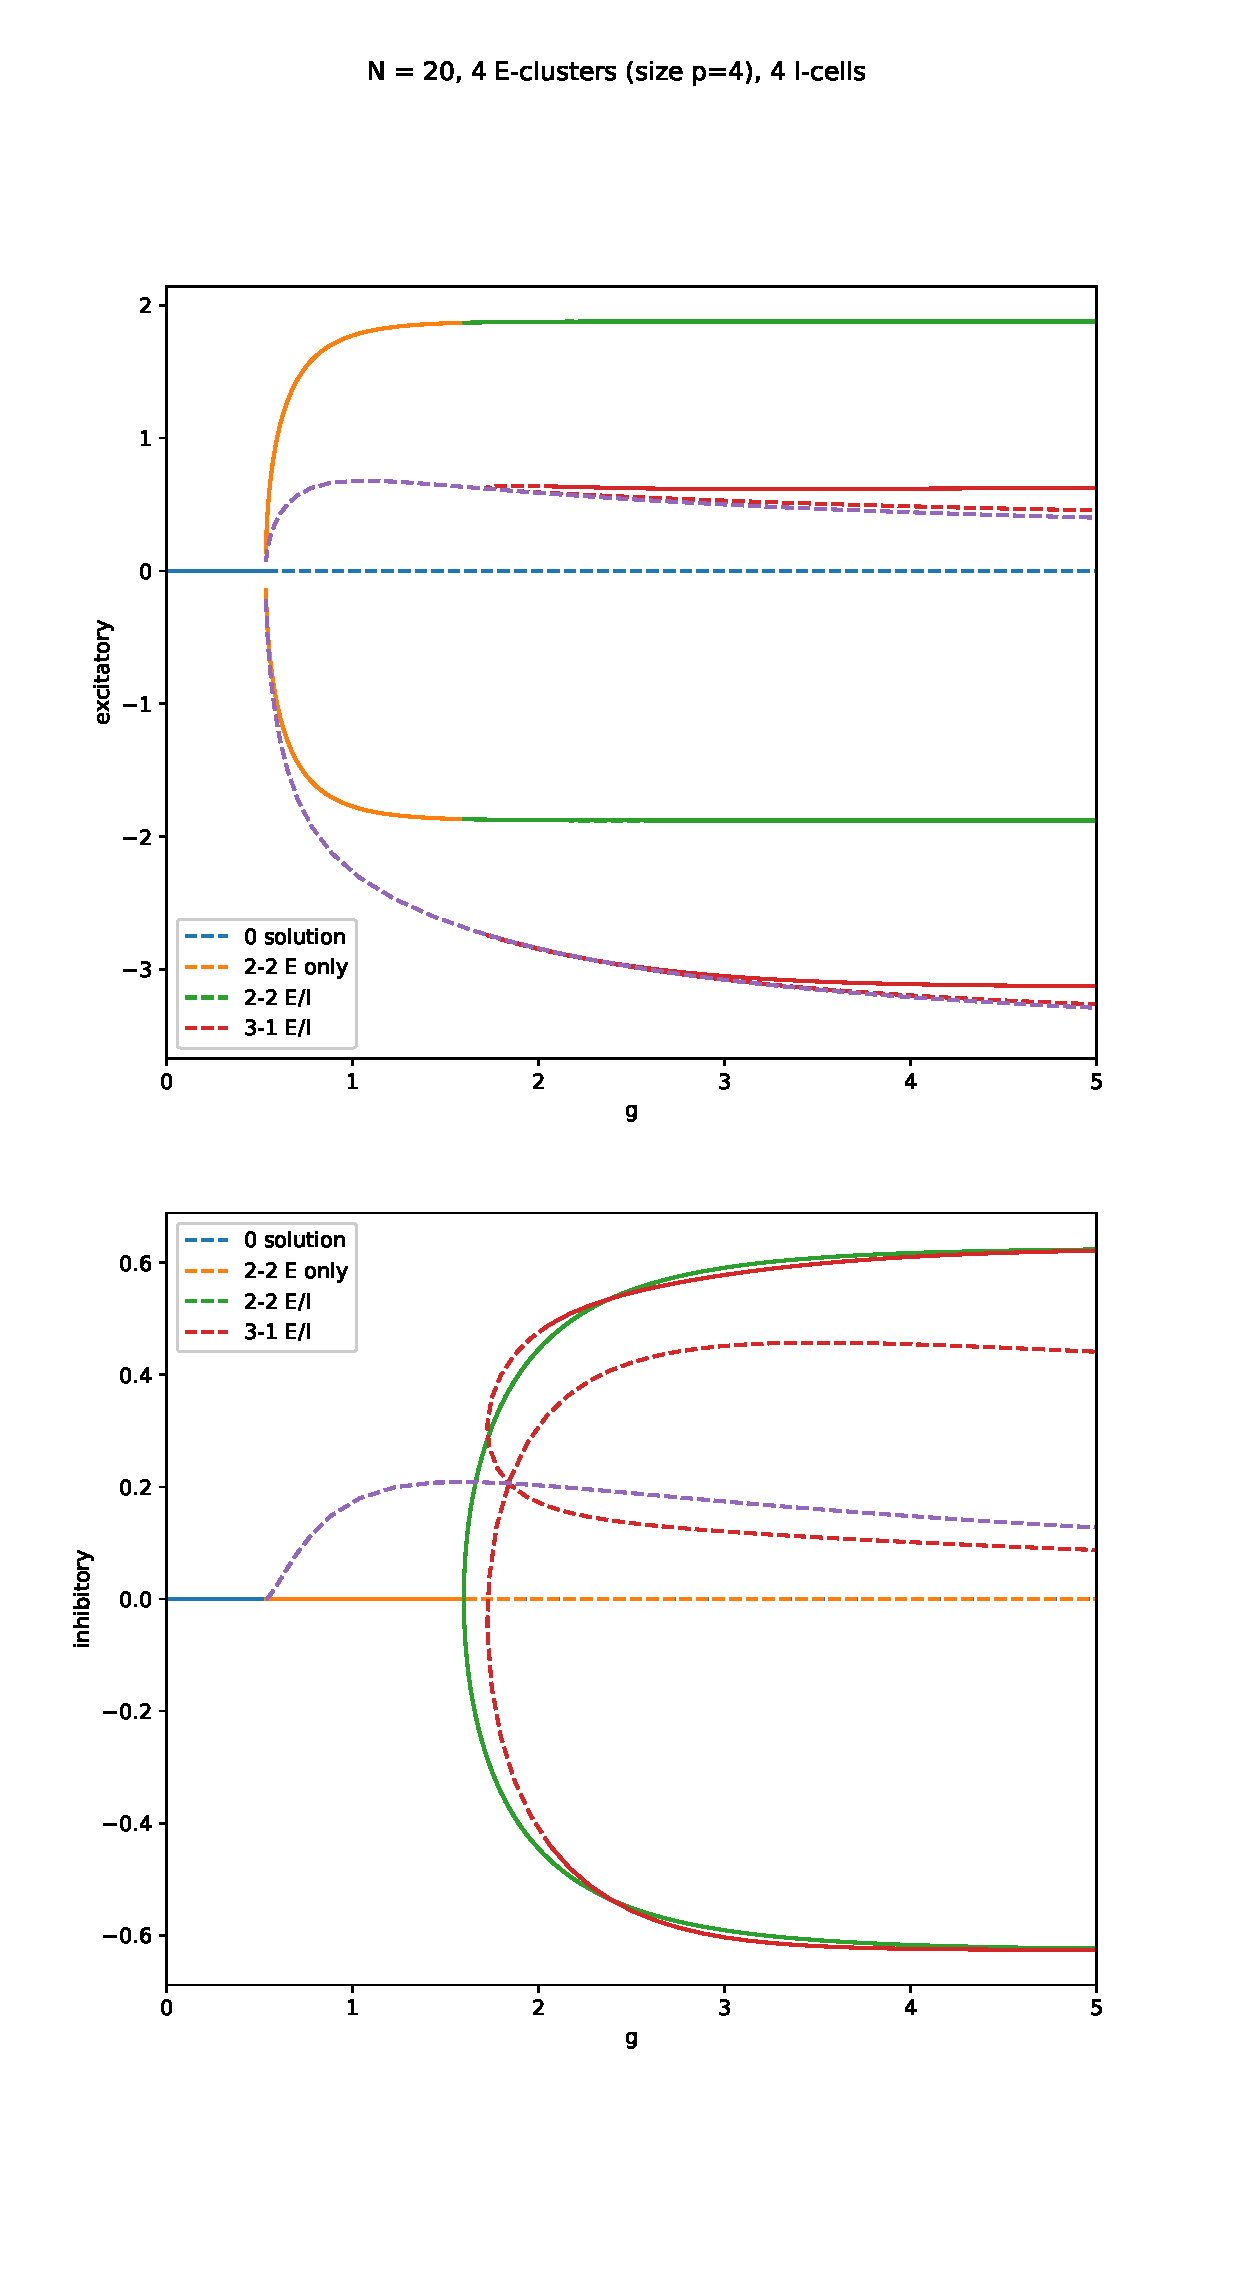
\includegraphics[width=14cm]{images/bifdiagc4p4i4.eps}
\end{figure}

\begin{figure}[H]
\centering
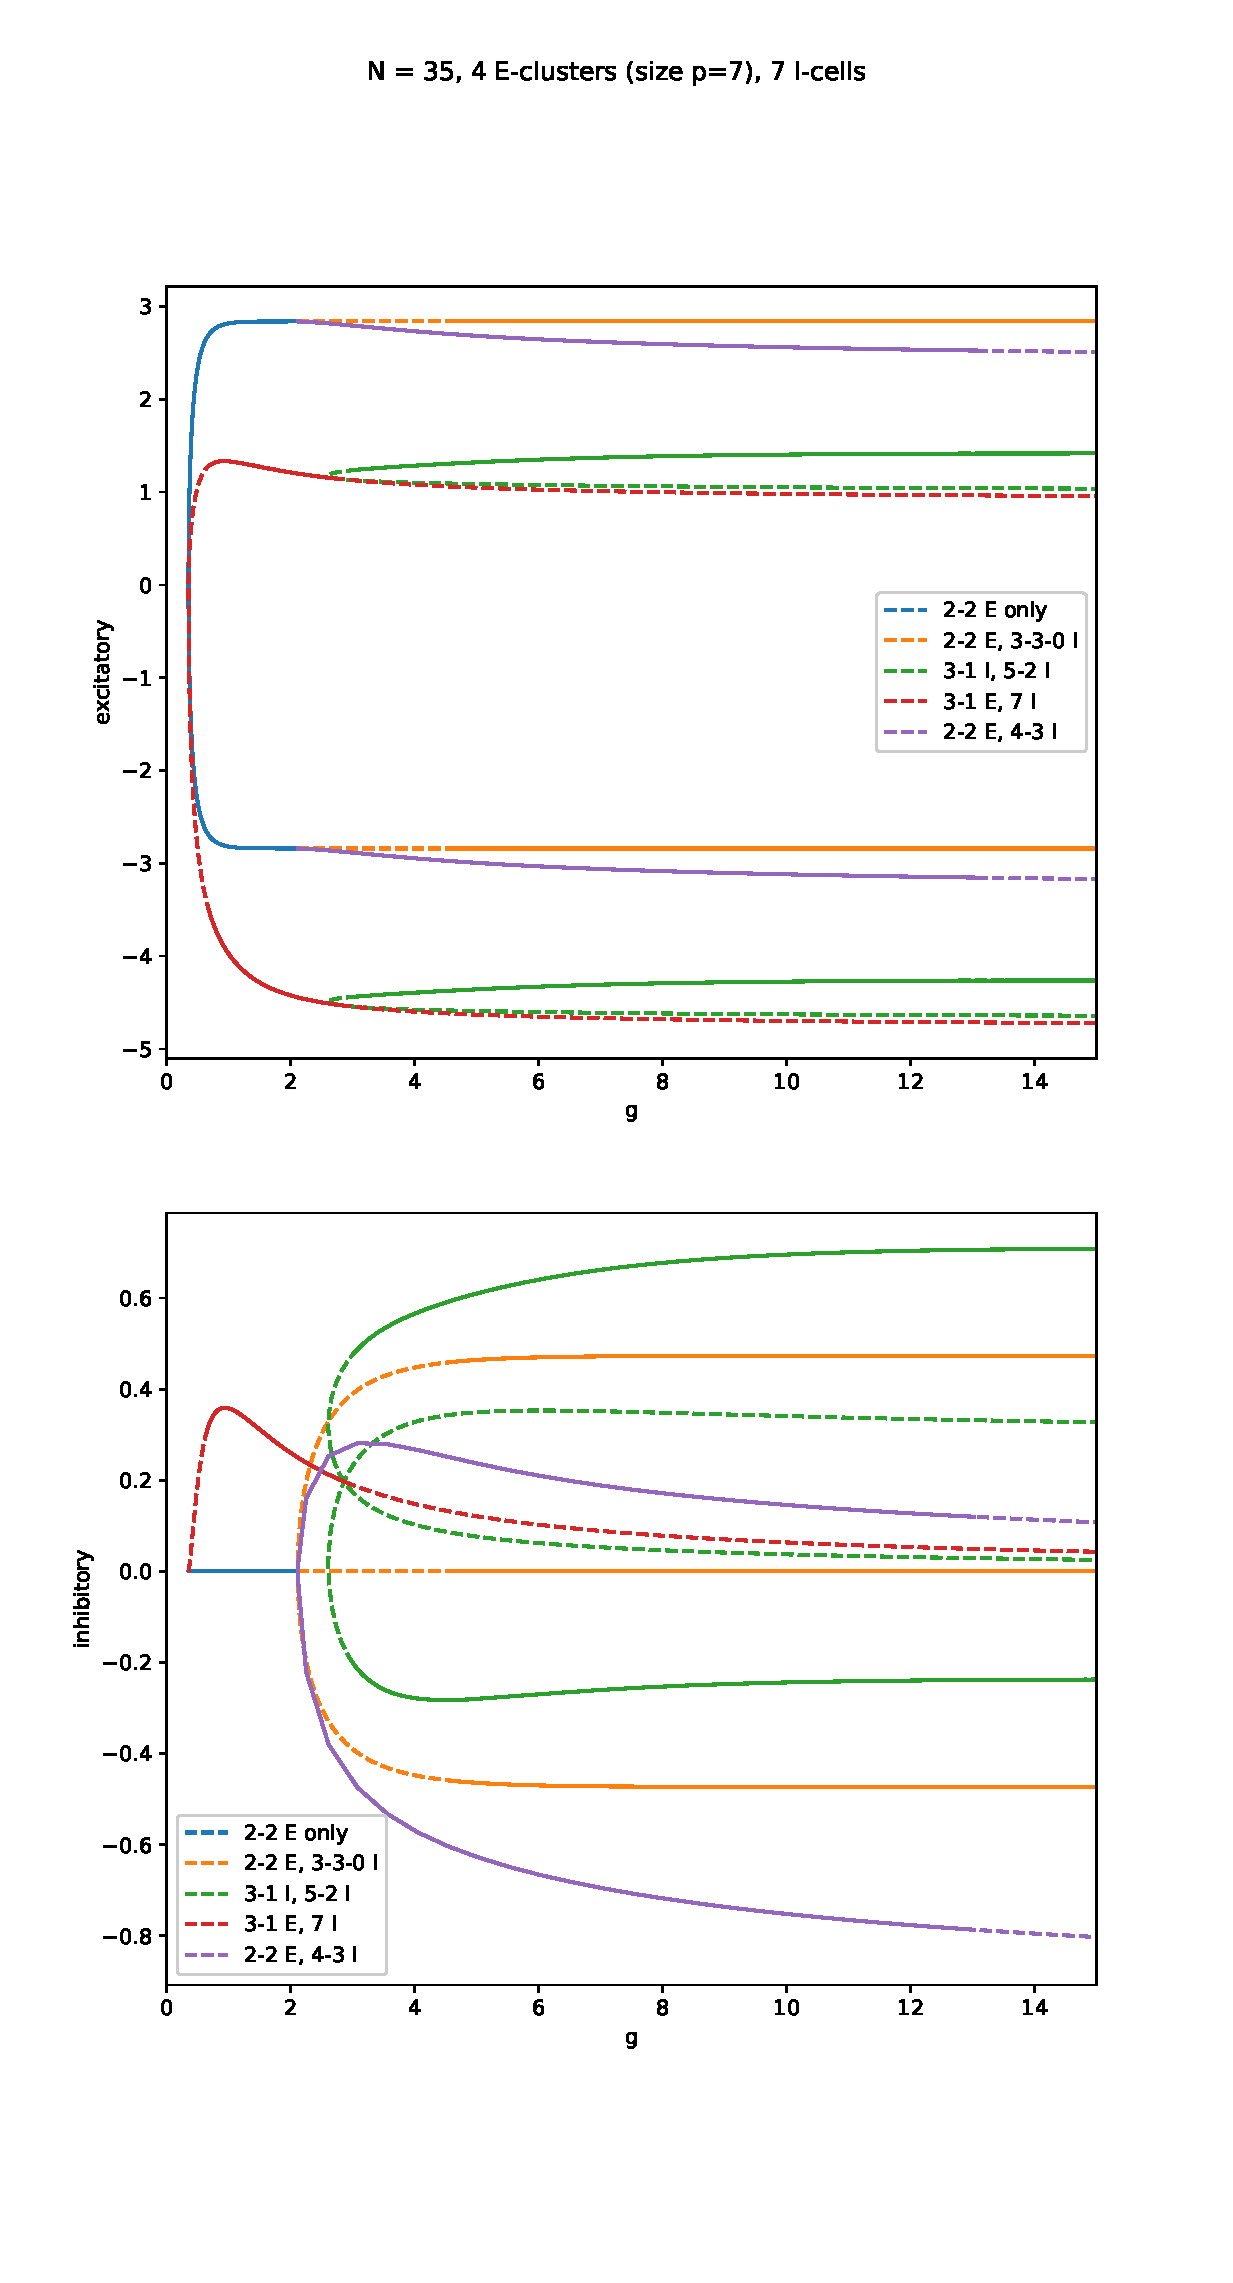
\includegraphics[width=14cm]{images/bifdiagc4p7i7.eps}
\end{figure}

\section{Inhibitory clusters, all excitatory cells connected}

To get this, all you have to do is exchange the Is and the Es in the previous case. This means that the eigenvalue pattern of the linearization about 0 is known, since we can use the same formulas as in the previous case, with the Is and Es switched.

In this case, we have
\begin{itemize}
    \item $N_{ci}$ inhibitory clusters of size $p_i$, so $N_I = N_{ci} p_i$.
    \item Everything else is the same.
\end{itemize}

\noindent For the linearization about 0, the eigenvalues of the matrix $H$ are (real part from L to R):
\begin{itemize}
    \item $\lambda_{ci} = (p_i - 1)\mu_{II}$ (multiplicity $p_i - 1$)
    \item $\lambda_E = -\mu_{EE}$ (multiplicity $N_E - 1$)
    \item $\lambda_I = -\mu_{II}$ (multiplicity $N_i - N_{ci}$.
    \item pair of complex eigenvalues which are the eigenvalues of
    \[
    \tilde{J}_i = \begin{pmatrix}
    (p_i - 1)\mu_{II} & N_{E} \mu_{IE} \\
    N_I \mu_{EI} & (N_E - 1)\mu_{EE}
    \end{pmatrix}
    \]
\end{itemize}

Key here is that the complex pair crosses the imaginary axis first as $g$ is increased, leading to a Hopf bifurcation and a stable limit cycle. The real part of this complex pair $\lambda \pm i \omega$ is given by
\begin{align*}
\lambda &= -\frac{\mu_{II} (1-f)N}{2}\left( 1 - \frac{1}{N_{ci}} + \frac{1}{N(1-f)}\left( 1 - \frac{1}{\alpha} \right) \right) \\
&\approx -\frac{\mu_{II} (1-f)N}{2}\left( 1 - \frac{1}{N_{ci}} \right) && \text{for $N$ large } \\
&\approx -\frac{\mu_{II} (1-f)N}{2} && \text{for $N$ and $N_{ci}$ large } \\
\end{align*}
which grows with $N$. This means that the Hopf bifurcation takes place at approximately
\[
g \approx g_0 \approx -\frac{2}{(1-f)\mu_{II}\sqrt{N}} 
\]
for large $N$ and $N_c$. The frequency of oscillations of the limit cycle is given by the imaginary part of the complex pair, which is approximately
\begin{align*}
\omega &\approx -\frac{\mu_{II} (1-f)N}{2 N_{ci} } \sqrt{ 3 N_{ci}^2 - 2 N_{ci} - 1} && \text{for $N$ large } \\
&\approx -\frac{\sqrt{3} \mu_{II} (1-f)N}{2 } && \text{for $N$ and $N_{ci}$ large }
\end{align*}
which also grows with $N$. At the Hopf bifurcation, which is at $g = g_0$, after scaling by $N$ and $g$, we have
\[
\omega \rightarrow \sqrt{3} \text{ as } N, N_{ci} \rightarrow \infty
\]
which is independent of everything. This assumes the same balance of inhibitory and excitatory neurons as before, as well as $\mu_{II} = -\alpha \mu_{EE}$, etc from the initial excitatory cluster case. 

Appears that this periodic orbit is stable for all $g > g_0$. For this orbit, all inhibitory cells and all excitatory cells synced. Frequency decreases as $g$ increases, also shape of oscillations changes.

\begin{figure}[H]
\centering
\begin{tabular}{cc}
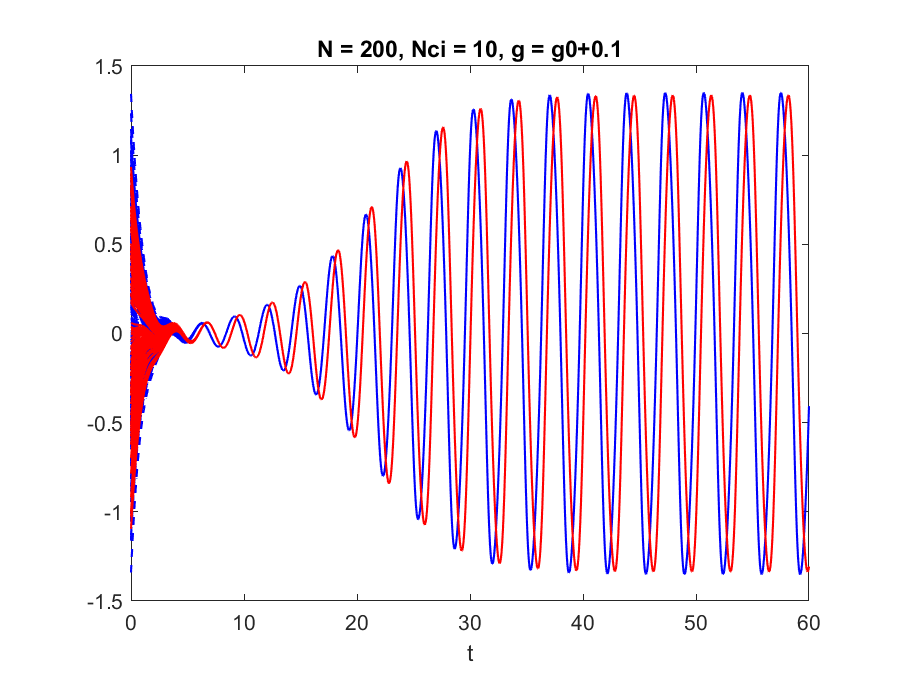
\includegraphics[width=8cm]{images/Iclustertimestep400_1.eps} &
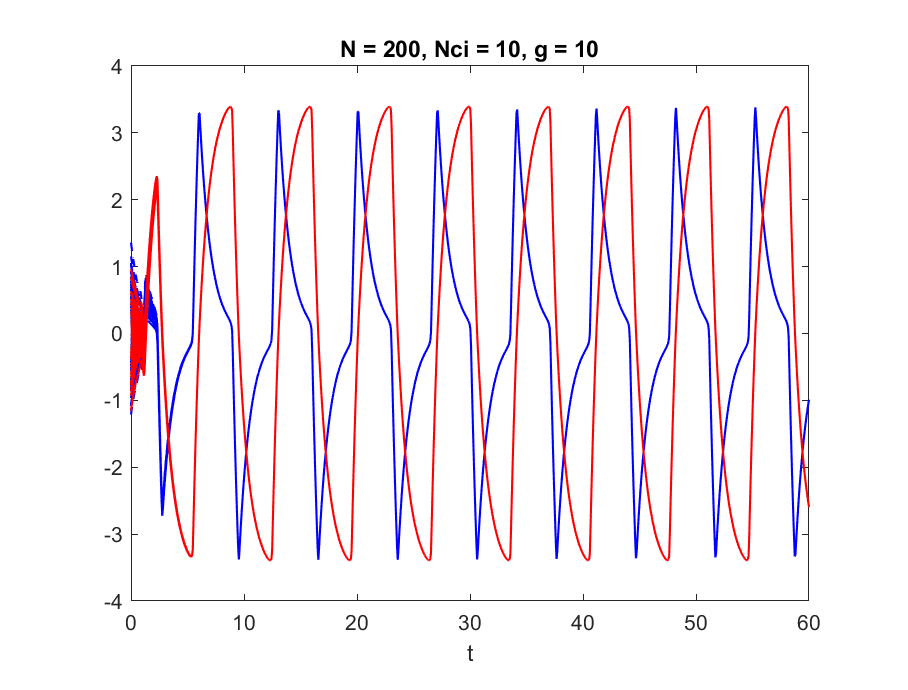
\includegraphics[width=8cm]{images/Iclustertimestep400_2.eps}
\end{tabular}
\end{figure}

\section{Excitatory clusters, balance restored, self-interactions allowed}

Self-interactions allowed in both E-clusters and I-cells. These are at least some of the stable fixed points. There may be others that AUTO did not find.

\begin{figure}[H]
\centering
\begin{tabular}{c}
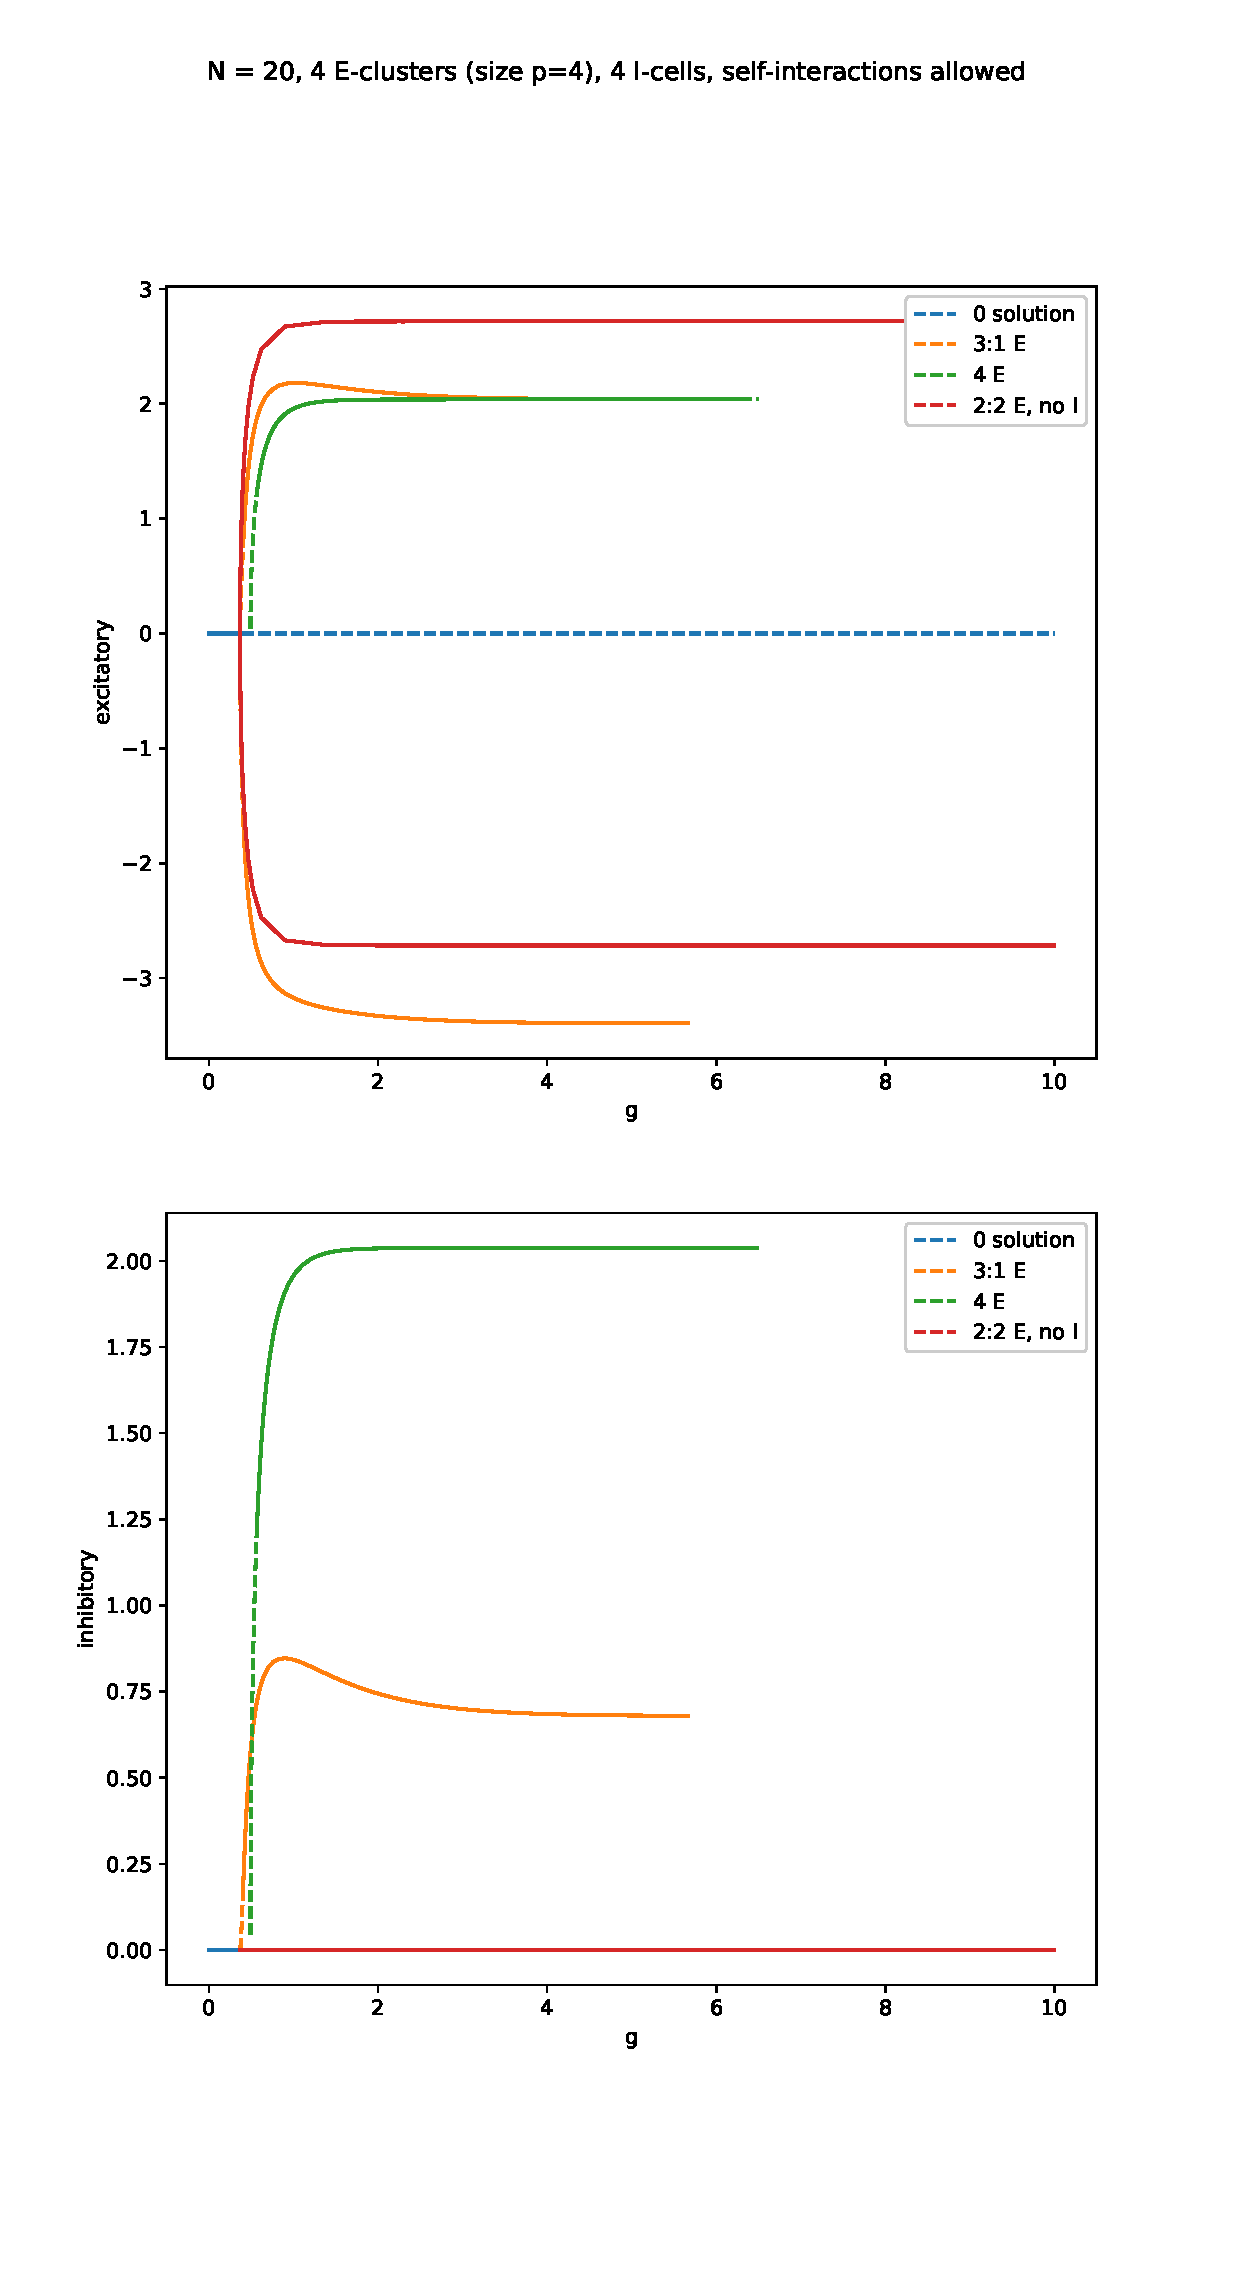
\includegraphics[width=12cm]{images/bifdiagc4p4i4selfint.eps}
\end{tabular}
\end{figure}

\section{Appendix}
\subsubsection{Detailed calculations for \S \ref{sec:stab_largeg}}

We are seeking solutions to 
 \begin{align}
 \begin{bmatrix} x_E\\x_{I_1}\\x_{I_2}\end{bmatrix} 
 &= \frac{\mu_E}{\sqrt{N}} 
 \begin{bmatrix} (n_E - 1) & -\alpha n_{I_1} & - \alpha n_{I_2}  \\
 n_E  & -\alpha (n_{I_1}-1) & - \alpha n_{I_2}  \\
 n_E  & -\alpha n_{I_1} & - \alpha (n_{I_2}-1)  
 \end{bmatrix}
 \begin{bmatrix} y_E\\y_{I_1}\\y_{I_2}\end{bmatrix} 
 \label{eqn:matSolgLrg}
 \end{align} 
 where $y_E = \tanh(gx_E)$, etc..
 Recall that if such a solutions can be found, its stability will be governed by the Eqn. 
 
 As $g \rightarrow \infty$, both the solutions and Jacobian simplify because the nonlinearities saturate to a constant value: if $x \rightarrow \hat{x} \not= 0$, then
\[ \tanh(gx) \rightarrow \left\{ \begin{matrix*} 1 & x > 0\\
    -1 & x < 0
    \end{matrix*}
    \right.
 \] 
 We will characterize solutions based on how many coordinates (i.e. $x_E, x_{I_1}$, and $x_{I_2}$) saturate in this way.
 
 Note that if all three coordinates $y_{E/I_1/I_2}=\pm 1$, then $J=-I$ and the solution will be stable for large $g$.
 Therefore we will start there. We ask if there is a vector of $\pm 1$, $(y_E, y_{I_1}, y_{I_2})$, whose image under this equation lies in the same octant (\textbf{S3}).
 \begin{itemize}
     \item Assume WLOG that $y_{I_1}>0$ and $y_{I_2}<0$. Define the balance $b = n_{I_1}-n_{I_2}$. Then our equations for $y_{I_1},y_{I_2}$ become
     \begin{align*}
        n_E y_E - \alpha(b-1) &>0\\
        n_E y_E - \alpha(b+1) &<0
     \end{align*}
     or, using the identity $n_E = \alpha n_I$,
     \[ n_I y_E - 1 < b < n_I y_E + 1 \]
     \item If $y_E=1$ then $n_I-1 < b < n_I+1$; if $y_E=-1$ then $-n_I-1 < b < -n_I+1$. Combining these two observations, either
     \[ b < -n_I + 1 \qquad \text{or} \qquad b > n_I - 1 \]
     
     However, the possible values of $b$ are limited by $n_I$: $n_{I_1}=n_I-1 \rightarrow b = n_I-1-1  = n_I-2$,  in fact
     \[ -n_I + 2 \leq b \leq n_I -2 \]
     neither option is possible! 
     \item The final option is that $y_E = 0$. This can only hold if $b=0$ i.e. $n_{I_1}=n_{I_2}$. The Jacobian in this case is
     \[ J = -I + \frac{g\mu}{\sqrt{N}}
     \begin{bmatrix} (n_E-1) & 0 & 0\\
        n_E & 0 & 0\\
        n_E & 0 & 0 \end{bmatrix}\]
        where we use $\sech^2(g x_{I_1}) = 0$, $\sech^2(gx_E)=1$.
        This solution is unstable for $g > \frac{\sqrt{N}}{\mu (n_E-1)}$
 \end{itemize}
 THis shows that while there is no solution of the form $\textbf{S3}$, there is one solution of the form $\textbf{S2}$.
 
Next, we consider the possibility that 
 $\tanh(gx) \rightarrow y$ but $0 < y < 1$ or $-1 < y < 0$ for each coordinate. In this case 
\[ x \approx \frac{\tanh^{-1}(y)}{g} \]

However, in Eqn. \eqref{eqn:matSolgLrg} the left-hand side must go to the zero vector as $g \rightarrow \infty$; thus the vector with the limiting values of $y_E$, $y_{I_1}$ and $y_{I_2}$ must be in the nullspace of the matrix in Eqn. \eqref{eqn:matSolgLrg}. 
This matrix is full rank! So there is no solution for which $x \rightarrow 0$ but $\tanh(gx) \rightarrow a$, where $0 < |a| < 1$, for all three values $x = x_E, x_{I1}, x_{I2}$. (\textbf{S0}).

Finally we show that the remaining $I_1/I_2$ branches have solutions of the form $\textbf{S1}$.
It turns out that what can happen is that, for example, $x_{E}, x_{I_1} \rightarrow 0$ as $g \rightarrow \infty$, but that $x_{I2}$ has a nonzero limit as $g \rightarrow \infty$ (see \cref{fig:20symm1} for an example of this exact occurrence for 1:1 and 3:1 I-cell symmetry in the $N=20$ case). Then we have $\tanh(g x_E), \tanh(g x_{I1})$ approaching a limit between 0 and 1 as $g \rightarrow \infty$ and $\tanh(g x_{I2}) \rightarrow 1$ as $g \rightarrow \infty$.

What are necessary conditions for such a solution to exist? Let us solve
\[ A \begin{bmatrix} y_1\\y_2\\y_3\end{bmatrix} = A \textbf{y} = \textbf{e}_k 
\]
where $\textbf{e}_k$ is the $k$th unit vector.

Then the following must be true:
\begin{enumerate}
    \item[\textbf{C1:}] $(\textbf{y})_k > 0$
    \item[\textbf{C2:}] $|(\textbf{y})_k| > |(\textbf{y})_j|$ for any $j\not=k$. 
\end{enumerate}
We can then obtain our desired $\begin{bmatrix} y_E\\y_{I_1}\\y_{I_2}\end{bmatrix} $ by dividing $\textbf{y}$ by its maximum.

% This is a necessary but not sufficient condition. The figure below shows the solution $y_E = 0.2222$, $y_{I_1}=-0.0556$, $y_{I_2}=1$, which we can obtain by using $\textbf{e}_3$ and normalizing the vector so that its largest entry is 1.

% However, there is a second possibility, using $\textbf{e}_2$, for which $y_E = 0.75$, $y_{I_1}=1$, $y_{I_2}=-0.1875$, which does not appear to correspond to an actual solution branch.

It turns out it is easy to invert $A$, using Cramer's rule:

\begin{align*}
   A^{-1} & = \frac{1}{\alpha^2 (N-1)}\begin{bmatrix}
    -\alpha^2 (n_I-1) & \alpha^2 n_{I_1} & \alpha^2 n_{I_2}\\
    -\alpha n_E & \alpha (n_E + n_{I_2}-1) & -\alpha n_{I_2}\\
    -\alpha n_E & -\alpha n_{I_1} & \alpha (n_E + n_{I_1}-1)\\
    \end{bmatrix}
\end{align*}

Note that $\textbf{C1}$ is met for $\evec_2$ and $\evec_3$, but is never met for $\evec_1$.
However, using $n_E = \alpha n_I$ and $\alpha > 1$, we can see that
\[ \alpha (n_E + n_{I_2}-1)> \alpha^2 n_{I_1} > \vert -\alpha n_{I_1}\vert \]
and
\[ \alpha (n_E + n_{I_1}-1)> \alpha^2 n_{I_2} > \vert -\alpha n_{I_2}\vert \]
i.e. \textbf{C2} is also met for both $\evec_2$ and $\evec_3$.

Therefore we have two solutions, each of which can be seen (for example) as the positive and negative parts of the 1:3 solution curve in Fig. \#\#:
\begin{eqnarray}
\begin{bmatrix} y_E\\y_{I_1}\\y_{I_2}\end{bmatrix} & = & \begin{bmatrix} \frac{\alpha n_{I_1}}{N-n_{I_1}-1}\\
    1 \\ -\frac{n_{I_1}}{N-n_{I_1}-1}
\end{bmatrix}
\label{eq:S1_sol1}
\end{eqnarray}
and 
\begin{eqnarray}
\begin{bmatrix} y_E\\y_{I_1}\\y_{I_2}\end{bmatrix} & = & \begin{bmatrix} \frac{\alpha n_{I_2}}{N-n_{I_2}-1}\\
    -\frac{n_{I_2}}{N-n_{I_2}-1}\\1
\end{bmatrix}.
\end{eqnarray}
For each solution, the value of the ``saturated" coordinate ($x_{I_1}$ or $x_{I_2}$) in the limit $g \rightarrow \infty$ is given by multiplying 
the vector above by $A$; for Eqn. \eqref{eq:S1_sol1},
\[ x_{I_1} = \frac{\alpha \mu_{EE}}{\sqrt{N}} \frac{N-1}{N-n_{I_1}-1}\]
Then for a finite $g$, recover the other coordinates using
\[ x_E = \frac{1}{g} \tanh^{-1}\left( \frac{\alpha n_{I_1}}{N-n_{I_1}-1}\right); \qquad  x_{I_2} = \frac{1}{g} \tanh^{-1}\left( -\frac{n_{I_1}}{N-n_{I_1}-1}\right)\]

To assess stability, return to Eqn. \eqref{eqn:Jmat_3pop}: writing $J = -I + \frac{g\mu_E}{\sqrt{N}} \tilde{J}$, we find that 
\[ {\rm tr} (\tilde{J})  = (1-y_E^2)(n_E-1) - (1-y_{I_1}^2)\alpha(n_{I_1}-1) \]


\bibliographystyle{amsplain}
\bibliography{main.bib}

\end{document}
